%\documentclass{article}
%
%\usepackage{fancyhdr}
%\usepackage{extramarks}
%\usepackage{amsmath}
%\usepackage{amsthm}
%\usepackage{amsfonts}
%\usepackage{tikz}
%\usepackage{enumerate}
%\usepackage{graphicx}
%\graphicspath{ {images/} }
%\usepackage[plain]{algorithm}
%\usepackage{algpseudocode}
%\usepackage[document]{ragged2e}
%\usepackage{textcomp}
%\usepackage{color}   %May be necessary if you want to color links
%\usepackage{import}
%\usepackage{hyperref}
%\hypersetup{
%    colorlinks=true, %set true if you want colored links
%    linktoc=all,     %set to all if you want both sections and subsections linked
%    linkcolor=black,  %choose some color if you want links to stand out
%}
%\usepackage{import}
%\usepackage{natbib}
%
%\usetikzlibrary{automata,positioning}
%
%
%% Basic Document Settings
%
%
%\topmargin=-0.45in
%\evensidemargin=0in
%\oddsidemargin=0in
%\textwidth=6.5in
%\textheight=9.0in
%\headsep=0.25in
%\setlength{\parskip}{1em}
%
%\linespread{1.1}
%
%\pagestyle{fancy}
%\lhead{\hmwkAuthorName}
%\lfoot{\lastxmark}
%\cfoot{\thepage}
%
%\renewcommand\headrulewidth{0.4pt}
%\renewcommand\footrulewidth{0.4pt}
%
%\setlength\parindent{0pt}
%
%
%\newcommand{\hmwkTitle}{Math Review Notes---Mathematical Statistics}
%\newcommand{\hmwkAuthorName}{\textbf{G. Faletto} }
%
%
%%%%%% Title Page
%
%
%\title{
%    \vspace{2in}
%    \textmd{\textbf{ \hmwkTitle}}\\
%}
%
%\author{Gregory Faletto}
%\date{}
%
%\renewcommand{\part}[1]{\textbf{\large Part \Alph{partCounter}}\stepcounter{partCounter}\\}
%
%
%%%%%% Various Helper Commands
%
%
%%%%%% Useful for algorithms
%\newcommand{\alg}[1]{\textsc{\bfseries \footnotesize #1}}
%
%%%%%% For derivatives
%\newcommand{\deriv}[2]{\frac{\mathrm{d} #1}{\mathrm{d} #2}}
%
%%%%%% For partial derivatives
%\newcommand{\pderiv}[2]{\frac{\partial #1}{\partial #2}}
%
%%%%%% Integral dx
%\newcommand{\dx}{\mathrm{d}x}
%
%%%%%% Alias for the Solution section header
%\newcommand{\solution}{\textbf{\large Solution}}
%
%%%%%% Probability commands: Expectation, Variance, Covariance, Bias
%\newcommand{\E}{\mathbb{E}}
%\newcommand{\Var}{\mathrm{Var}}
%\newcommand{\Cov}{\mathrm{Cov}}
%\newcommand{\Bias}{\mathrm{Bias}}
%\newcommand\indep{\protect\mathpalette{\protect\independenT}{\perp}}
%\def\independenT#1#2{\mathrel{\rlap{$#1#2$}\mkern2mu{#1#2}}}
%\DeclareMathOperator{\Tr}{Tr}
%
%\theoremstyle{definition}
%\newtheorem{theorem}{Theorem}
%\numberwithin{theorem}{subsection}
%\theoremstyle{definition}
%\newtheorem{proposition}[theorem]{Proposition}
%\theoremstyle{definition}
%\newtheorem{lemma}[theorem]{Lemma}
%\theoremstyle{definition}
%\newtheorem{corollary}{Corollary}[theorem]
%\theoremstyle{definition}
%\newtheorem{definition}{Definition}[section]
%\newtheorem*{remark}{Remark}
%\theoremstyle{definition}
%\newtheorem{exercise}{Exercise}
%\theoremstyle{definition}
%\newtheorem{example}{Example}[section]
%
%%%%%% Tilde
%\newcommand{\textapprox}{\raisebox{0.5ex}{\texttildelow}}
%
%\begin{document}
%
%\maketitle
%
%\pagebreak
%
%\tableofcontents
%
%\
%
%\
%
%\begin{center}
%Last updated \today
%\end{center}
%
%
%
%\newpage
%%
%%%
%%%
%%%
%%%
%%%
%%%
%%%
%%%
%%%%
%%%% Mathematical Statistics

\section{Mathematical Statistics}

These are my notes from taking Math 541A at USC taught by Steven Heilman as well as \textit{Statistical Inference} (2nd edition) by Casella and Berger \citep{CaseBerg:01}, Statistics 100B at UCLA taught by Nicolas Christou, ISE 620 at USC taught by Sheldon Ross, Math 505A at USC taught by Sergey Lototsky, and a few other sources I cite within the text.

\subsection{Order Statistics}

\begin{definition}[\textbf{Order statistics (from Math 541A, more precise)}] Let \(X:\Omega\to\mathbb{R}\) be a random variable.  Let $X_{1},\ldots,X_{n}$ be a random sample of size $n$ from $X$.  Define $X_{(1)}:=\min_{1\leq i\leq n}X_{i}$, and for any $2\leq i\leq n$, inductively define
$$X_{i}:=\min\Big\{\{X_{1},\ldots,X_{n}\}\setminus\{X_{(1)},\ldots,X_{(i-1)}\}\Big\},$$
so that
$$X_{(1)}\leq X_{(2)}\leq\cdots\leq X_{(n)}=\max_{1\leq i\leq n}X_{i}.$$
The random variables $X_{(1)},\ldots,X_{(n)}$ are called the \textbf{order statistics} of $X_{1},\ldots,X_{n}$.


\end{definition}

\begin{definition}[\textbf{Order statistics (from ISE 620, more informal)}] Let \(X_1, \ldots X_n \sim iid \ \ F\) with \(F' = f\). Define \(X_{(1)}\) as the smallest among \(X_1, \ldots, X_n\), \(X_{(2)}\) as the 2nd smallest, and so on, up to \(X_{(n)}\), the largest of the group. We call \(X_{(1)}, \ldots, X_{(n)}\) the \textbf{order statistics} of \(X_1, \ldots, X_n\).

\end{definition}

\begin{proposition}[\textbf{Order statistics distribution function; from Math 541A}]\label{mathstats.order.stats.dist} Suppose $X$ is a discrete random variable and we can order the values that $X$ takes as $x_{1}<x_{2}<\cdots$.  For any $i\geq1$, define $p_{i}:= \Pr(X\leq x_{i})$. Then for any $1\leq i,j\leq n$,
$$\Pr(X_{(j)}\leq x_{i})=\sum_{k=j}^{n}\binom{n}{k}p_{i}^{k}(1-p_{i})^{n-k}.$$
\end{proposition}

\begin{proof} Note that \(\{X_{(j)} \leq x_i\}\) is equivalent to the event that \(j\) or more of the \(X_i\) are less than or equal to \(x_i\) regardless of order; that is, \(x_i\) is the \(k\)th smallest observed value. Let \(A_k\) be the event that exactly \(k\) of the \(X_i\) are less than or equal to \(x_i\) regardless of order. Then

\[
\{X_{(j)} \leq x_i\} = \bigcup_{k=j}^n A_k.
\]

Then since (by definition of \(p_i\))

\[
\Pr(A_k) = \binom{n}{k} p_i^k(1-p_i)^{n-k}
\]

and using the fact that the \(\{A_k\}\) are disjoint, we have

\[
\Pr(\{X_{(j)} \leq x_i\}) = \Pr(\bigcup_{k=j}^n A_k) = \sum_{k=1}^n \Pr(A_k) = \sum_{k=1}^n \binom{n}{k} p_i^k(1-p_i)^{n-k}.
\]

\end{proof}

\begin{corollary}\label{mathstats.order.stats.density.541a} if $X$ is a continuous random variable with density $f_{X}$ and cumulative distribution function $F_{X}$, then for any $1\leq j\leq n$, $F_{X_{(j)}}$ has density
$$f_{X_{(j)}}(x):=\frac{n!}{(j-1)!(n-j)!}f_{X}(x)(F_{X}(x))^{j-1}(1-F_{X}(x))^{n-j},\qquad\forall\,x\in\mathbb{R}.$$

\end{corollary}

\begin{proof} This follows by differentiating the identity from Proposition \ref{mathstats.order.stats.dist} for the cumulative distribution function.

\end{proof}

\begin{proposition}[\textbf{Order statistics joint density function; result from ISE 620}]\label{mathstats.order.stats.density} The joint density of the order statistics is

\[
f_{X_{(1)}, \ldots, X_{(n)}}(x_1, \ldots, x_n) = n! \prod_{i=1}^n f(x_i).
\]

\end{proposition}

\begin{proof} Start with \(n=2\). We seek \(f_{X_{(1)}, X_{(2)}}(x_1,  x_2) \). Note that \(X_{(1)} = x_1, X_{(2)} = x_2\) if \(X_1 = x_1, X_2 = x_2\) or if \(X_1 = x_2, X_2 = x_1\). These are mutually exclusive events, so their density is equal to the sums of the two densities. That is,

\[
f_{X_{(1)}, X_{(2)}}(x_1,  x_2) = f_{X_1, X_2} (x_1, x_2) +  f_{X_1, X_2} (x_2, x_1) = 2 f(x_1) f(x_2)
\]

where the last step follows from the i.i.d. distributions. Generalizing, we have

\[
f_{X_{(1)}, \ldots, X_{(n)}}(x_1, \ldots, x_n) = n! \prod_{i=1}^n f(x_i).
\]

\end{proof}

\begin{proposition}[\textbf{Distribution of order statistics of uniform random variable; from 541A}]\label{mathstats.orders.unif.dist}Let $X$ be a random variable uniformly distributed in $[0,1]$. Then for any $1\leq j\leq n$, $X_{(j)}$ is a beta distributed random variable with parameters $j$ and $n+1-j$. 
\end{proposition}

\begin{proof} Note that for a uniform distribution on \([0,1]\), \(f_X(x) = 1, x \in [0,1]\) and \(F_X(x) = x, x \in [0,1]\). Therefore by Corollary \ref{mathstats.order.stats.density.541a} we have

\[
f_{X_{(j)}}(x) =\frac{n!}{(j-1)!(n-j)!} (x)^{j-1}(1-x)^{n-j},\qquad x\in [0,1]
\]

\[
 =\frac{\Gamma(n+1)}{\Gamma(j) \Gamma(n+1-j)} x^{j-1}(1-x)^{n-j}  =\frac{\Gamma(j + n + 1 - j)}{\Gamma(j) \Gamma(n + 1 - j)} x^{j-1}(1-x)^{n+1-j - 1}
 \]


which is the pdf for a beta distribution with parameters \(j\) and \(n + 1 -j\). 

\end{proof}

\begin{corollary}Let $X$ be a random variable uniformly distributed in $[0,1]$. Then \(\E X_{(j)}=\frac{j}{n+1}\)

\end{corollary}

\begin{proof} Follows from Proposition \ref{mathstats.orders.unif.dist} since the mean of such a beta distribution is \(\frac{j}{n+1}\).

\end{proof}

\begin{proposition}[\textbf{Result from 541A}] Let $a,b\in\mathbb{R}$ with $a<b$.  Let $U$ be the number of indices $1\leq j\leq n$ such that $X_{j}\leq a$.  Let $V$ be the number of indices $1\leq j\leq n$ such that $a<X_{j}\leq b$.  Then the vector $(U,V,n-U-V)$ is a multinomial random variable, so that for any nonnegative integers $u,v$ with $u+v\leq n$, we have
    \begin{flalign*}
    &\mathbb{P}(U=u,V=v,n-U-V=n-u-v)\\
    &\qquad=\frac{n!}{u!v!(n-u-v)!}F_{X}(a)^{u}(F_{X}(b)-F_{X}(a))^{v}(1-F_{X}(v))^{n-u-v}.
    \end{flalign*}
    Consequently, for any $1\leq i,j\leq n$,
    $$\mathbb{P}(X_{(i)}\leq a,X_{(j)}\leq b)=\mathbb{P}(U\geq i,U+V\geq j)=\sum_{k=i}^{j-1}\sum_{m=j-k}^{n-k}\mathbb{P}(U=k,V=m)+\mathbb{P}(U\geq j).$$
    So, it is possible to write an explicit formula for the joint distribution of $X_{(i)}$ and $X_{(j)}$.
    
    \end{proposition}
    
    \begin{proof} We can define a multinomial distribution as follows (from Sheldon Ross \textit{Stochastic Processes}, see Definition \ref{prob.ross.multinomial.dist.def}): ``Suppose that \(n\) independent trials, each of which results in either outcome \(1, 2, \ldots, r\) with respective probabilities \(p_1, p_2, \ldots, p_r\) (with \(\sum_{i} p_i = 1\)), are performed. Let \(N_i\) denote the number of trials resulting in outcome \(i\). Then the joint distribution of \(N_1, \ldots, N_r\) is called the \textbf{multinomial distribution.}" In this case \(r=3\). If we define outcome 1 to be \(X_j \leq a\), outcome 2 to be \(a < X_j \leq b\), and outcome 3 to be \(X_j > b\), then the counts \((U, V, n-U-V)\) meet this definition exactly, with \(p_1 = \Pr(X_j \leq a) = F_X(a)\), \(p_2 = \Pr(a < X_j \leq b) = F_X(b) - F_X(a)\), \(p_3 = \Pr(X_j > b) = 1 - F_X(b)\). Since the pmf of a multinomial distribution with \(r=3\) is 

\[
\Pr((N_1, N_2, N_3) = (n_1, n_2, n_3) ) = \binom{n}{n_1, n_2, n_3} p_1^{n_1}  p_2^{n_2}  p_3^{n_3 }  = \frac{n!}{n_1! n_2! n_3!}  p_1^{n_1}  p_2^{n_2}  p_3^{n_3 }
\]

we have in this case

\[
\Pr (U=u,V=v,n-U-V=n-u-v) =\frac{n!}{u!v!(n-u-v)!}F_{X}(a)^{u}(F_{X}(b)-F_{X}(a))^{v}(1-F_{X}(v))^{n-u-v}
    \]
    
    as desired.
    
    \end{proof}
    
\begin{definition}[\textbf{Median; Math 505A defintion}] The real number \(m\) is called a \textbf{median} of a random variable \(X\) if

\[
\Pr(X \leq m) \geq 1/2, \qquad \Pr(X \geq m) \geq 1/2.
\]

\end{definition}

\begin{proposition}[\textbf{Math 505A homework problem}] 

\begin{enumerate}[(a)]

\item Every random variable has at least one median. 

\item The set of all medians is a closed interval of the real line.

\end{enumerate}

\end{proposition}

\begin{proof} 

\begin{enumerate}[(a)]

\item Suppose the cdf of \(X\), \(F_X: \mathbb{R} \to [0, 1]\), is continuous. Because \(F_X(x) = \Pr(X \leq x)\) is a cdf, it is also monotonically increasing. By the Intermediate Value Theorem, there exists at least one \(m \in \mathbb{R}\) such that \(F_X(m) = 1/2\). Because \(\Pr(X \leq m) = 1/2 \geq 1/2\) and \(\Pr(X \geq m) = 1 - \Pr(X < m) = 1 - 1/2 \geq 1/2\), \(m\) is a median.

\

Suppose \(F_X\) is not continuous. If it contains \(1/2\) in its range, then \(m\) such that \(F_X(m) = 1/2\) is a median. If there is no \(m \in \mathbb{R}\) such that \(F_X(m) = 1/2\), then \(m = \inf( \{x \mid F_X(x) \geq 1/2 \} )\) is a median. To see why, note first that \( \Pr(X \leq m) = F_X(m) \geq 1/2\). Second, 

\[
\Pr(X \geq m) = 1 - \Pr(X < m) = 1 - \lim_{x \to m^-} F_X(x) \geq 1 - 1/2 = 1/2
\]

because \(F_X\) is right continuous. Therefore \(m\) is a median of \(X\).

\item We show that all medians of \(X\) must be in one interval by contradiction. Suppose \(a\) and \(b\) are medians of \(X\) but \( c\) is not, where \(a < c < b\). By the definition of median, \(F_X(a) \geq 1/2\) and \(F_X(b) \geq 1/2\). Because \(c\) is not a median, \(F_X(c) < 1/2\). This implies that \(F_X\) is decreasing on the interval from \(a\) to \(c\), which contradicts the fact that the distribution function \(F_X\) monotonically increases.

\

Finally we prove that all medians of \(X\) are in a closed interval. Let \(\mathcal{A}\) be the set of all medians of \(X\); that is, \(\mathcal{A} = \{ x \mid  \Pr(X \leq x) \geq 1/2, \Pr(X \geq x) \geq 1/2 \}\) =  \( \{ x \mid  F_X(x) \geq 1/2, \lim_{y \to x^-}F_X(y) \leq 1/2 \}\). We will show that \(\mathcal{A}\) contains its infimum and its supremum. The argument above shows that \(a = \inf( \{x \mid F_X(x) \geq 1/2 \} )\) satisfies \( \lim_{y \to a^-}F_X(y) \leq 1/2 \); that is, \(a \in \mathcal{A}\). Since there is no lower value \(k\) which satisfies \(F_X(k) \geq 1/2\), \(a = \inf(\mathcal{A})\), so \(\mathcal{A}\) contains its infimum. 

\

Let \(b = \sup\{x \mid \lim_{y \to x^-}F_X(y) \leq 1/2\}\). Because \(b\) is the supremum of a set containing \(a\), \(b \geq a\). Therefore because \(F_X\) is nondecreasing, \(F_X(b) \geq F_X(a) \geq 1/2\), which shows that \(b \in \mathcal{A}\). Since \(b\) is the supremum of the set of all values satisfying \(\lim_{y \to x^-}F_X(y) \leq 1/2\), \(b\) is the supremum of \(\mathcal{A}\). Therefore \(\mathcal{A}\) contains its infimum and supremum, and the set of all medians of \(X\) is closed.

\end{enumerate}

\end{proof}

\begin{remark} One example of a random variable which has a median of length \(L\): \(X\) is a discrete random variable with the following mass function:

\[
\Pr(X = 0) = 0.5
\]

\[
\Pr(X = L) = 0.5
\]

Then \(m \in [0, L]\) are medians.

\end{remark}

\subsection{Random Samples}

\begin{definition}[\textbf{Random Sample}] Let \(n >0\) be an integer.  A \textbf{random sample} of size \(n\) is a sequence \(X_1, \ldots, X_n\) of independent identically distributed random variables.

\end{definition}

\begin{definition}[\textbf{Statistic}] Let \(n, k\) be positive integers. Let \(X_1, \ldots, X_n\) be a random sample of size \(n\). Let \(f: \mathbb{R}^n \to \mathbb{R}^k\) be a (measureable) function. A \textbf{statistic} is a random variable of the form \(Y:= f(X_1, \ldots, X_n)\). The distribution of \(Y\) is called a \textbf{sampling distribution.}

\end{definition}

\begin{definition}[\textbf{Sample mean}] The \textbf{sample mean} of a random sample \(X_1, \ldots, X_n\) of size \(n\), denoted \(\overline{X}\), is the following statistic:

\[
\overline{X} := \frac{1}{n} \sum_{i=1}^n X_i.
\]

\end{definition}

\begin{proposition}\label{mathstats.sample.mean.props} Suppose we have a random sample of size \(n\) from an i.i.d. distribution \(X_1, X_2, \ldots, X_n\) with \(\E(X_1) = \mu \ in \mathbb{R}\), \(\Var(X_1) = \sigma^2 < \infty\). Then

\begin{enumerate}[(a)]

\item \(\E(\overline{X}) = \E(X_1)\).

\item \( \Var(\overline{X}) = \sigma^2/n\).

\end{enumerate}

\end{proposition}

\begin{proof}

\begin{enumerate}[(a)]

\item

\[
\E(\overline{X}) = \E \bigg( \frac{1}{n} \sum_{i=1}^n X_i\bigg) = \frac{1}{n} \sum_{i=1}^n \E   X_i  = \frac{1}{n} \cdot n \mu = \mu
\]

\item

Using the independence of the \(X_i\),

\[
\Var (\overline{X}) = \Var \bigg( \frac{1}{n} \sum_{i=1}^n X_i\bigg) =  \frac{1}{n^2} \Var \bigg( \sum_{i=1}^n X_i\bigg) =  \frac{1}{n^2} \sum_{i=1}^n  \Var ( X_i ) = \frac{1}{n^2}  \cdot n \sigma^2 = \boxed{\frac{\sigma^2}{n}}
\]

\end{enumerate}

\end{proof}

\begin{proposition}[\textbf{Stats 100B homework problem}] Suppose that \(X_1, \ldots , X_m\) and \(Y_1, \ldots , Y_n\) are two samples, with \(X \sim  \mathcal{N}(\mu_1, \sigma_1)\) and \(Y \sim  \mathcal{N}(\mu_2, \sigma_2)\). The difference between the sample means, \(\bar{X} - \bar{Y}\) , is then a linear combination of \(m + n\) normal random variables. Then

\begin{enumerate}[a.]

\item \(\E(\bar{X} - \bar{Y}) =  \mu_1 - \mu_2\).

\item \(\Var (\bar{X} - \bar{Y}) = \frac{\sigma_1^2}{m} + \frac{\sigma_2^2}{n}  \).

\item The distribution of \(\bar{X} - \bar{Y}\) is normal with mean and variance equal to the previous results.

\end{enumerate}

\end{proposition}

\begin{proof}

\begin{enumerate}[a.]

\item
% Question 6 part (a)

\[
\bar{X} = \frac{1}{m} \sum_{i=1}^m X_i, \ \bar{Y} = \frac{1}{n} \sum_{j=1}^n Y_j 
\]


\[
\E(\bar{X} - \bar{Y}) = \E\bigg(\frac{1}{m} \sum_{i=1}^m X_i - \frac{1}{n} \sum_{j=1}^n Y_j \bigg) = \frac{1}{m} \E\bigg( \sum_{i=1}^m X_i\bigg) - \frac{1}{n} \E \bigg(\sum_{j=1}^n Y_j \bigg)
\]

\[
= \frac{1}{m}  \sum_{i=1}^m \E (X_i)  - \frac{1}{n} \sum_{j=1}^n \E(Y_j) = \frac{1}{m}  \sum_{i=1}^m \mu_1  - \frac{1}{n} \sum_{j=1}^n \mu_2 = \frac{1}{m} m \cdot \mu_1 - \frac{1}{n} n \cdot \mu_2
\]

\[
\implies
\E(\bar{X} - \bar{Y}) = \mu_1 - \mu_2
\]

\item 
% Question 6 part (b)

Since \(X\) and \(Y\) are independent,

\[
\Var (\bar{X} - \bar{Y}) = \Var(\bar{X}) + \Var(\bar{Y})
\]

\[
= \E\big[ (\bar{X} - \E[\bar{X}])^2 \big] + \E\big[ (\bar{Y} - \E[\bar{Y}])^2 \big]
\]

\[
= \E\bigg( \frac{1}{m} \sum_{i=1}^m X_i - \mu_1 \bigg)^2 + \E\bigg( \frac{1}{n} \sum_{j=1}^n Y_j - \mu_2 \bigg)^2
\]

\[
= \E\bigg( \frac{1}{m} \sum_{i=1}^m \big(X_i - m \frac{1}{m} \mu_1\big) \bigg)^2 + \E\bigg( \frac{1}{n} \sum_{j=1}^n \big( Y_j - n \frac{1}{n} \mu_2 \big) \bigg)^2
\]

\[
= \frac{1}{m^2 }\E\bigg(\sum_{i=1}^m \big(X_i - \mu_1\big) \bigg)^2 + \frac{1}{n^2} \E\bigg(  \sum_{j=1}^n \big( Y_j - \mu_2 \big) \bigg)^2
\]

Since \(X_i\) and \(X_j\) are independent for \(i \neq j\) (and likewise for \(Y\)), \(\Cov(X_i, X_j) = 0\) for \(i \neq j\), so 

\[
\E[(X_i - \mu_1)(X_j - \mu_1)] = 0
\] 

for \(i \neq j\) (and likewise for \(Y\)). Therefore the above equation can be written as

\[
\frac{1}{m^2 }\E\bigg(\sum_{i=1}^m \big(X_i - \mu_1\big)^2 \bigg) + \frac{1}{n^2} \E\bigg(  \sum_{j=1}^n \big( Y_j - \mu_2 \big)^2 \bigg)
\]

\[
\frac{1}{m^2 }\sum_{i=1}^m \E \big(X_i - \mu_1\big)^2  + \frac{1}{n^2}   \sum_{j=1}^n \E \big( Y_j - \mu_2 \big)^2
\]

\[
= \frac{1}{m^2 }\bigg(\sum_{i=1}^m \sigma_1^2 \bigg) + \frac{1}{n^2} \bigg(  \sum_{j=1}^n \sigma_2^2 \bigg) = \frac{1}{m^2}m \cdot \sigma_1^2 + \frac{1}{n^2} n \cdot \sigma_2^2
\]

\[
\implies
\Var (\bar{X} - \bar{Y}) = \frac{\sigma_1^2}{m} + \frac{\sigma_2^2}{n} 
\]

\item
% Question 6 part (c)

\[
M_{X_i}(t) = \exp\bigg(\mu_1 t + \frac{t^2 \sigma_1^2}{2} \bigg), \ M_{Y_i}(t) = \exp\bigg(\mu_2 t + \frac{t^2 \sigma_2^2}{2} \bigg)
\]

Since individual observations from \(X\) and \(Y\) are independent,

\[
M_{\bar{X}}(t) = \prod_{i=1}^m M_{X_i}\bigg(\frac{1}{m}t\bigg), \ M_{\bar{Y}}(t) = \prod_{j=1}^n M_{Y_j}\bigg(\frac{1}{n}t\bigg)
\]

and

\[
M_{\bar{X} - \bar{Y}}(t) = M_{\bar{X}}(t) M_{\bar{-Y}}(t) = M_{\bar{X}}(t) M_{\bar{Y}}(-t) = \prod_{i=1}^m M_{X_i}\bigg(\frac{1}{m}t\bigg) \prod_{j=1}^n M_{Y_j}\bigg(\frac{-1}{n}t\bigg)
\]

\[
= \bigg[ M_{X_i}\bigg(\frac{t}{m} \bigg) \bigg] ^m  \bigg[ M_{Y_j}\bigg( \frac{-t}{n} \bigg)  \bigg]^n = \bigg[ \exp\bigg(\frac{\mu_1 t}{m} + \frac{t^2 \sigma_1^2}{2m^2} \bigg) \bigg] ^m  \bigg[ \exp\bigg(\frac{-\mu_2 t}{n} + \frac{(-t)^2 \sigma_2^2}{2n^2} \bigg) \bigg]^n
\]

\[
= \exp\bigg(\frac{m \mu_1 t}{m} + \frac{m t^2 \sigma_1^2}{2m^2} \bigg)   \exp\bigg(\frac{-n \mu_2 t}{n} + \frac{n t^2 \sigma_2^2}{2n^2} \bigg)
\]

\[
\implies \boxed{
M_{\bar{X} - \bar{Y}}(t) = \exp \bigg[ (\mu_1 - \mu_2)t + \frac{1}{2}t^2 \bigg( \frac{\sigma_1^2}{m}  + \frac{\sigma_2^2}{n} \bigg) \bigg]}
\]

This is the moment generating function of a normal distribution with mean \( \mu_1 - \mu_2\) and variance \(\frac{\sigma_1^2}{m}  + \frac{\sigma_2^2}{n}\), consistent with the results from parts (a) and (b).


\end{enumerate}

\end{proof}

\begin{definition}[\textbf{Sample variance}] Let \(n > 1\). The \textbf{sample variance} of a random sample \(X_1, \ldots, X_n\) of size \(n\), denoted \(S^2\), is the following statistic:

\[
S^2 := \frac{1}{n-1} \sum_{i=1}^n (X_i - \overline{X})^2.
\]

The \textbf{sample standard deviation} of a random sample of size \(n\) is \(\sqrt{S^2}\).

\end{definition}

\begin{proposition}[\textbf{Unbiasedness of sample variance}] Suppose we have a random sample of size \(n\) from an i.i.d. distribution \(X_1, X_2, \ldots, X_n\) with \(\E(X_1) = \mu \ in \mathbb{R}\), \(\Var(X_1) = \sigma^2 < \infty\). Then \(\E(S^2) = \sigma^2\). Further, \(S^2\) is a consistent estimator of \(\sigma^2\).

\end{proposition}

\begin{proof}

We have

\[
\E(S^2) = \E \bigg( \frac{1}{n-1} \sum_{i=1}^n (X_i - \overline{X})^2 \bigg) = \frac{1}{n-1}  \E \bigg( \sum_{i=1}^n X_i^2 - 2X_i\overline{X} + \overline{X}^2 \bigg)
\]

\[
= \frac{1}{n-1} \bigg( \sum_{i=1}^n  \E(X_i^2)  - 2 \E \bigg( \overline{X}  \sum_{i=1}^n  X_i \bigg) + n \E\overline{X}^2 \bigg)  = \frac{1}{n-1} \bigg(  n \E(X_i^2)  - 2n \E  \overline{X}^2  + n \E\overline{X}^2 \bigg)
\]

\[
= \frac{n}{n-1} \big(   \E(X_i^2)  -  \E  \overline{X}^2 \big) = \frac{n}{n-1} \big(  \Var(X_i) + \E(X_i)^2 - [\Var(\overline{X}) + \E( \overline{X})^2] \big)
\]

Using the results from Proposition \ref{mathstats.sample.mean.props}, we have

\[
\E(S^2) = \frac{n}{n-1} \big(  \sigma^2 + \mu^2 - [ \sigma^2/n + \mu^2] \big)  = \frac{n}{n-1} \cdot \frac{(n-1) \sigma^2}{n}  = \boxed{\sigma^2}
\]

\end{proof}

\begin{proof}[Alternative proof from Stats 100B homework.]

\[
\E\bigg( \frac{1}{n} \sum_{i=1}^n(x_i - \mu)^2  \bigg) = \frac{1}{n}  \E\bigg( \sum_{i=1}^n(x_i - \mu)^2  \bigg)
\]

Assuming independence of samples, this can be written as

\[
\frac{1}{n}  \sum_{i=1}^n  \E( (x_i - \mu)^2) = \frac{1}{n} n \sigma^2 = \boxed{\sigma^2}
\]

Since \(S^2\) is unbiased, it is a consistent estimator if we can show \(\Var(S^2) \to 0\)  as \( n \to \infty\). We have

\[
\Var(\frac{(n-1)S^2}{\sigma^2}) = 2(n-1)
\]

\[
\frac{(n-1)^2}{\sigma^4}\Var(S^2) = 2(n-1)
\]

\[
\Var(S^2) = \frac{2\sigma^4}{n-1}
\]

\[
\implies \lim_{n \to \infty} \Var(S^2) =  \lim_{n \to \infty}  \frac{2\sigma^4}{n-1} = \boxed{0}
\]

Therefore \(S^2\) is a consistent estimator of \(\sigma^2\).

\end{proof}

\begin{lemma}\label{stats.hw3.ex.3.16} Let \(X := (X_1, \ldots, X_n)\) be i.i.d. mean zero, variance 1 Gaussian random variables. Let \(v_1, \ldots, v_n \in \mathbb{R}^n\). Then \(\langle X, v_1 \rangle, \ldots, \langle X, v_n \rangle\) are independent if and only if \(v_1, \ldots, v_m \) are pairwise orthogonal; that is,  \(\langle v_i, v_j \rangle = 0 \ \forall \ 1 \leq i < j \leq m\). 

\end{lemma}

\begin{proof} By Theorem \ref{prob.thm.sums.gaussian}, we have that for any $v\in\mathbb{R}^{n}$, $\langle X, v\rangle$ is a mean zero Gaussian with variance $\langle v,v\rangle$. For notational convenience, let \(\langle X, v_k \rangle = A_k\). Because all the \( A_k \) are Gaussian random variables by Theorem \ref{prob.thm.sums.gaussian}, the \(A_k\) are uncorrelated if and only if they are independent. That is, we would like to show that their covariances


\[
\E[(A_k - \E A_k)(A_\ell - \E A_\ell)] 
\]

equal zero for all \( \{(k, \ell) : k, \ell \in \{1, 2, \ldots, m\}, k \neq \ell \}\) if and only if the vectors $v_1,\dots,v_m$ are pairwise orthogonal; that is, \(\langle v_k, v_\ell \rangle = 0 \) for all \( \{(k, \ell) : k, \ell \in \{1, 2, \ldots, m\}, k \neq \ell \}\). Note that since \(A_k = \sum_{i=1}^n X_i v_{ki}\), \(\E (A_k) =   \sum_{i=1}^n  v_{ki} \E(X_i)\). So for any \( \{(k, \ell) : k, \ell \in \{1, 2, \ldots, m\}, k \neq \ell \}\) we have

\[
\E[(A_k - \E A_k)(A_\ell - \E A_\ell)] = \E \bigg[ \bigg( \sum_{i=1}^n X_i v_{ki} -   \sum_{i=1}^n  v_{ki} \E(X_i) \bigg) \bigg(\sum_{i=1}^n X_i v_{\ell i} -   \sum_{i=1}^n  v_{\ell i} \E(X_i) \bigg) \bigg] 
\]

\[
= \E \bigg[ \bigg( \sum_{i=1}^n X_i v_{ki} \bigg)  \bigg(\sum_{i=1}^n X_i v_{\ell i} \bigg) -  \bigg( \sum_{i=1}^n X_i v_{ki} \bigg) \bigg( \sum_{i=1}^n  v_{\ell i} \E(X_i) \bigg)   
\]

\[
-   \bigg( \sum_{i=1}^n  v_{ki} \E(X_i) \bigg) \bigg(\sum_{i=1}^n X_i v_{\ell i} \bigg)  +    \bigg( \sum_{i=1}^n  v_{ki} \E(X_i) \bigg)  \bigg(  \sum_{i=1}^n  v_{\ell i} \E(X_i) \bigg) \bigg] 
\]




\[
= \E \bigg(  \sum_{i=1}^n X_i^2 v_{ki} v_{\ell i} + \sum_{\{a, b \in \{1, \ldots, n\}, a \neq b \} }   X_a X_b v_{ka}  v_{\ell b}\bigg)
-  2 \E \bigg(  \sum_{i=1}^n X_i \E(X_i) v_{ki} v_{\ell i} + \sum_{\{a, b \in \{1, \ldots, n\}, a \neq b\} }   X_a \E(X_b) v_{ka}  v_{\ell b} \bigg)   
\]

\[  
+   \E  \bigg(  \sum_{i=1}^n \E(X_i)^2 v_{ki} v_{\ell i} + \sum_{\{a, b \in \{1, \ldots, n\},a \neq b \} }   \E(X_a) \E(X_b) v_{ka}  v_{\ell b} \bigg)
\]

Recall that \(\E(X_i)= 0\) for all \(i\). Also, due to independence of the \(X_i\), all of the terms that involve \(\E (X_a X_b), \ a \neq b\) disappear. This leaves only

 \begin{equation}\label{prob.541a.hw3.5}
= \E \bigg(  \sum_{i=1}^n X_i^2 v_{ki} v_{\ell i} \bigg) = \sum_{i=1}^n  \E (X_i^2 ) v_{ki} v_{\ell i}  = \E (X_1^2 ) \sum_{i=1}^n   v_{ki} v_{\ell i} 
\end{equation}

where the last step follows from the i.i.d. distributions of \(X_i\). Recall

\[
\langle v_k, v_\ell \rangle = 0 \iff  \sum_{i=1}^n   v_{ki} v_{\ell i}  = 0.
\]

Since \(\E(X_i^2) \neq 0\), (\ref{prob.541a.hw3.5}) equals 0 for all \( \{(k, \ell) : k, \ell \in \{1, 2, \ldots, m\}, k \neq \ell \}\) if and only if \(\langle v_k, v_\ell \rangle = 0 \) for all \( \{(k, \ell) : k, \ell \in \{1, 2, \ldots, m\}, k \neq \ell \}\). Therefore the random variables $\langle X, v_1 \rangle, \dots, \langle X, v_m \rangle$ are independent if and only if the vectors $v_1,\dots,v_m$ are pairwise orthogonal.

\end{proof}

\begin{proposition}[\textbf{Proposition 4.7 in 541A notes}] Let \(n \geq 2\) be an integer. Let \(X_1, \ldots, X_n\) be a random sample from the Gaussian distribution with mean \(\mu \in \mathbb{R}\) and variance \(\sigma^2 > 0\). Let \(\overline{X}\) be the sample mean and let \(S\) be the sample standard deviation. Then

\begin{enumerate}[(i)]

\item \(\overline{X}\) and \(S\) are independent random variables.

\item \(\overline{X}\) is a Gaussian random variable with mean \(\mu\) and variance \(\sigma^2/n\).

\item \((n-1)S^2/\sigma^2\) is a \(\chi^2\)-distributed random variable with \(n-1\) degrees of freedom.

\end{enumerate}

\end{proposition}

\begin{proof}

\begin{enumerate}[(i)]

\item Replace \(X_1, \ldots, X_n\) with \(X_1 - \mu, \ldots, X_n - \mu\) so that \(\mu = 0\). Also divide by \(\sigma\) so that \(\sigma=1\). Note that \(\overline{X}\) is independent of all random variables \(X_2 - \overline{X}, \ldots, X_n - \overline{X}\) by Lemma \ref{stats.hw3.ex.3.16} because for example

\[
X_2 - \overline{X} = \langle X_2, e_2 - \frac{1}{n} (1, 1, \ldots, 1) \rangle
\]

where the second vector in the inner product is orthogonal to \((1, 1, \ldots, 1 )\) (in fact, \((1, \ldots, 1)\) is orthogonal to anything in the span of these vectors). Likewise for all the remaining vectors you could use to construct \(X_i\). (Note that the other random variables [e.g. \(X_2 - \overline{X}\) and \(X_3 - \overline{X}\)] are not independent.)

\

So the proof will be complete if we can write \(S\) as a function of \(X_2 - \overline{X}, \ldots, X_n - \overline{X}\). Observe

\[
(n-1)S^2 = \sum_{i=1}^n (X_i - \overline{X})^2 = (X_1 - \overline{X})^2 + \sum_{i=2}^n (X_i - \overline{X})^2 = \bigg( n \overline{X} - \bigg[ \sum_{i=2}^n X_i \bigg] - \overline{X} \bigg) ^2 + \sum_{i=2}^n \bigg( X_i - \overline{X} \bigg)^2 
\]

\[
= \bigg(\sum_{i=2}^n (X_i - \overline{X}  \bigg)^2 + \sum_{i=2}^n (X_i - \overline{X})^2 
\]

\item Follows from Proposition 1.45, Example 1.108, and Exercise 1.58 in 541A notes (condense later?)

\item Like above, replace \(X_1, \ldots, X_n\) with \(X_1 - \mu, \ldots, X_n - \mu\) so that \(\mu = 0\). Also divide by \(\sigma\) so that \(\sigma=1\). We will prove by induction. Let \(\overline{X}_n:= \frac{1}{n} \sum_{i=1}^n X_i\) and let \(S_n^2 := \frac{1}{n-1} \sum_{i=1}^n (X_i - \overline{X}_n)^2\). In the case \(n=2\) we have

\[
S_2^2 = \bigg(X_1 - \frac{1}{2}(X_1 + X_2) \bigg)^2 + \bigg(X_2 - \frac{1}{2}(X_1 + X_2) \bigg)^2 = \frac{1}{4}(X_2 - X_1)^2 + \frac{1}{4}(X_2 - X_1)^2 = \frac{1}{2}(X_2 - X_1)^2 
\]

\[
= \bigg( \frac{1}{\sqrt{2}} (X-2 - X_1) \bigg)^2
\]

Note that \(1/\sqrt{2} (X_2 - X_1)\) is a mean zero Gaussian random variable with variance 1 (see example 1.108 in 541A notes for details). So \(S_2^2\) is \(\chi_1^2\) by Definition 1.33 in 541A notes.

\

We now induct on \(n\). From Lemma 4.8 in 541A notes (will prove later),

\[
n S_{n+1}^2 = (n-1) S_n^2 + \frac{n}{n+1}(X_{n+1} - \overline{X}_n)^2, \ \ \ \forall n \geq 2
\]

From the first item, \(S_n\) is independent of \(\overline{X}_n\). Also, \(X_{n+1}\) is independent of \(S_n\) by Proposition 1.61 in Math 541A notes, since \(S_n\) is a function of \(X_1, \ldots, X_n\), which are independent of \(X_{n+1}\). So \(S_n\) is independent of \((X_{n+1} - \overline{X}_n)^2\). By the inductive hypothesis, \((n-1)S_n^2\) is a \(\chi_{n-1}^2\) random variable. From Example 1.108 in Math 541A notes, \(X_{n+1} - \overline{X}_n\) is a Gaussian random variable with mean zero and variance \(1 + 1/n = (n+1)/n\) so that \(\sqrt{n/(n+1)} (X_{n+1} - \overline{X}_n)\) is a mean zero Gaussian with variance 1, implying \(n/(n+1) (X_{n+1} - \overline{X}_n)^2\) is \(\chi^2\). Definition 1.33 in 541A notes then implies that \(nS_{n+1}\) is a \(\chi_n^2\) random variable, completing the inductive step.

\end{enumerate}

\end{proof}

\begin{lemma}[\textbf{Lemma 4.8 in 541A notes.}]

\end{lemma} Let \(X_1, X_2, \ldots\) be random variables. For any \(n \geq 2\), let \(\overline{X}_n:= (1/n)\sum_{i=1}^n X_i\) and let \(S_n^2:= 1/(n-1) \sum_{i=1}^n (X_i - \overline{X}_n)^2\). Then

\[
n S_{n+1}^2  - (n-1)S_n^2 =\frac{n}{n+1}(X_{n+1} - \overline{X}_n)^2.
\]

\begin{proof}

\[
n S_{n+1}^2  - (n-1)S_n^2 = \sum_{i=1}^{n+1} (X_i - \overline{X}_{n+1})^2 - \sum_{i=1}^n (X_i - \overline{X}_n)^2 
\]

Note:

\[
(a-b)^2 - (a-c)^2 = a^2 - 2ab + b^2 - a^2 - c^2 + 2ac = b^2 - c^2 + 2a(c-b) 
\]

\[
= (b-c)[(b+c)  - 2a]= (b-c)(b+c-2a)
\]

for all real \(a, b,c\). Using \(a=X_n, b= \overline{X}_{n+1}, c= \overline{X_n}\) we have

\[
= (X_{n+1} - \overline{X}_{n+1})^2 + \sum_{i=1}^n(\overline{X}_{n+1}- \overline{X}_n)(\overline{X}_{n+1} + \overline{X}_n - 2 X_i) 
\]

\[
= (X_{n+1} - \overline{X}_{n+1})^2 + (\overline{X}_{n+1} - \overline{X}_n) \sum_{i=1}^n (\overline{X}_{n+1} + \overline{X}_n - 2 X_i)
\]

\[
= (X_{n+1} - \overline{X}_{n+1})^2 + (\overline{X}_{n+1} - \overline{X}_n) \cdot n (\overline{X}_{n+1} + \overline{X}_n - 2 \overline{X}_n)
\]

\[
=(X_{n+1}(1 - 1/(n+1)) - \frac{n}{n++1} \overline{X}_n)^2 + n(\overline{X}_{n+1} - \overline{X}_n)^2
\]

\[
= \frac{n^2}{(n+1)^2} (X_{n+1} - \overline{X}_n)^2 + n ( \frac{X_{n+1}}{n+1} + ( \frac{1}{n+1} - \frac{1}{n} ) \sum_{i=1}^n X_i )^2
\]

Algebra: \(1/(n+1) - 1/n = \frac{n - (n+1)}{n(n+1)} = - \frac{1}{n(n+1)}\). So we have

\[
= \frac{n^2}{(n+1)^2}(X_{n+1}-\overline{X}_n)^2  + \frac{n}{(n+1)^2} (X_{n+1} - \frac{1}{n} \sum_{i=1}^n X_i )^2
\]

\[
= \frac{n^2}{(n+1)^2} (X_{n+1}-\overline{X}_n)^2 + \frac{n}{(n+1)^2} (X_{n+1} - \overline{X}_n)^2
\]

\[
=\frac{n^2+n}{(n+1)^2} (X_{n+1} - \overline{X}_n)^2 = \frac{n}{n+1}(X_{n+1} - \overline{X}_n)^2
\]


\end{proof}

\begin{proposition}[\textbf{Proposition 4.9 in 541A notes}] Let \(X\) be a standard Gaussian random variable. Let \(Y\) be a \(\chi_p^2\) random variable. Assume that \(X\) and \(Y\) are independent. Then \(X/\sqrt{Y/p}\) has the following density, known as \textbf{Student's \(t\)-distribution} with \(p=\) degrees of freedom: (\(p=n+1\)?)

\[
f_{X/(Y/\sqrt{p})}(t):= \frac{ \Gamma((p+1)/2)}{\sqrt{p} \sqrt{\pi} \Gamma(p/2) } \bigg( 1 + \frac{t^2}{p} \bigg)^{-(p+1)/2}, \ \ \ \forall t \in \mathbb{R}
\]

(should have \(p+1\) in a bunch of the expressions above? that's what was written on board, not in notes.)

\end{proposition}

\begin{proof} Let \(Z:= \sqrt{Y/p}\). We find the density of \(Z\) as follows. Let \(t > 0\). Then

\[
f_Z(y) = \deriv{}{y}\big|_{y=0} \Pr(Z \leq y) = \deriv{}{y} \big|_{y=0} \Pr(Y \leq y^2p) 
\]

\[
=  \deriv{}{y} \big|_{y=0} \int_0^{y^2p} \frac{x^{(p/2)-1}e^{-x/2}}{2^{p/2} \Gamma(p/2)} dx = 2yp \cdot p^{(p/2)-1} y^{p-2}e^{-y^2p/2} \cdot \frac{1}{2^{p/2} \Gamma(p/2)}
\]

\[
=p^{p/2}y^{p-1}e^{-y^2 p/2} \cdot \frac{1}{2^{p/2-1} \Gamma(p/2)}
\] 

\[
\vdots \text{ skipped this stuff in class proof}
\]

\[
\Pr(X/Z \leq t) = \Pr(X \leq tZ) 
\]

\[
= \text{ (by definition of joint density) }  \int \int_{\{ (x,y) \in \mathbb{R}^2: x \leq ty \} } f_X(x) f_Z(y) dx dy
\]

We use the change of variables formula:

\[
\int \int_{\phi(U)} f(x,y) dxdy = \int \int_U f(\phi(a,b)) | \operatorname{Jac} \phi(a,b)| da db
\]

\[
\phi: \mathbb{R}^2 \to \mathbb{R}^2
\]

\[
\phi(a,b) = (ab,a)
\]

\[
\phi^{-1}(x,y) =(y, x/y)
\]

We chose \(x/y\) as the second variable so that an upper limit of the variable will end up being \(t\) after the transformation. We need the Jacobian of \(\phi\):'

\[
| \operatorname{Jac} \phi(a,b) | = \left| \operatorname{det} \begin{pmatrix} b & a \\ 1 & 0 \end{pmatrix} \right| = |a|
\]

By the change in variables formula,

\[
\int \int_{\phi(U)} f(x,y) dx dy = \int \int_U f(\phi(a,b)) \left| \operatorname{Jac} \phi(a,b) \right| da db
\]

\[
 = \int \int_{\{ (a,b) \in \mathbb{R}^2: a \geq 0, b \leq t \} }  f_X(ab) f_Z(a) \left| a \right| da db
\]

\[
\implies \Pr(X/Z \leq t) = \int_{-\infty}^t \int_0^\infty |a|  f_X(ab) f_Z(a) da db
\]

By the Fundamental Theorem of Calculus,

\[
f_{X/Z}(t) = \deriv{}{t} \Pr(X/Z \leq t) = \int_0^\infty |a|  f_X(at) f_Z(a)) da = \int_0^\infty a f_X(at) f_Z(a)) da
\]

By the definitions of \(X\) and \(Z\), 

\[
= \frac{1}{2^{-/2-1} \Gamma(p/2)}\int_0^\infty a  \cdot \frac{1}{\sqrt{2 \pi}} e^{-(a^2t^2)/2} \cdot p^{p/2} a^{p-1} e^{-a^2p/2}  da
\]

\[
= \frac{p^{p/2} }{2^{-/2-1} \Gamma(p/2) \sqrt{2 \pi}}\int_0^\infty   e^{-[a^2(t^2 + p)]/2} \cdot a^{p}  da
\]

Change of variables: let \(x = a^2, dx = 2ada, da= \frac{1}{2a} dx = 1/(2 \sqrt{x}) dx\). Then this integral is

\[
= c \int_0^\infty   e^{-[x(t^2 + p)]/2} \cdot x^{p/2 - 1/2}  da, \ \ \ \text{where } c = \frac{p^{p/2}}{2^{p/2} \sqrt{2 \pi} \Gamma(p/2)}
\]

So the integrand is a Gamma density function with parameters \(\alpha, \beta\): \(\alpha  - 1 = p/2 - 1/2 \iff \alpha = p/2 + 1/2\), \(\beta = 2/(t^2 + p)\). So if we multiply and divide \(\beta^\alpha \Gamma(\alpha)\)

\

So

\[
f_{X/Z}(t) = \frac{p^{p/2}}{2^{p/2} \sqrt{2 \pi} \Gamma(p/2)} \cdot \beta^\alpha \Gamma(\alpha) \cdot 1 = \frac{p^{p/2} \Gamma((p_1)/2)}{2^{p/2} \sqrt{2 \pi} \Gamma(p/2)} \cdot \bigg( \frac{2}{t^2 + p} \bigg)^{(p-1)/2}
\]

\[
= \frac{p^{p/2} \Gamma((p+1)/2)}{\sqrt{\pi} \Gamma(p/2)} \cdot (t^2 + p)^{-(p+1)/2} = \frac{\Gamma((p+1)/2)}{\sqrt{\pi p} \Gamma(p/2)} \cdot (1 + t^2/p)^{-(p+1)/2}
\]




\end{proof}

\begin{remark}[Remark 4.10 in 541A notes] If \(X_1, \ldots, X_n\) is a random sample from a Gaussian distribution with mean \(\mu \in \mathbb{R}\), standard deviation \(\sigma < 0\), then

\[
\frac{\overline{X} - \mu}{S / \sqrt{n}}
\]

also has Student's \(t\) distribution. (\(\overline{X} := n^{-1} \sum_{i=1}^n X_i, S = \sqrt{(n-1)^{n-1} \sum_{i=1}^n (X_i - \overline{X})^2}\).)

\end{remark}

\begin{proposition}[\textbf{Stats 100B homework 3 problem}] Let \(X_1, X_2\) be a random sample from a normal distribution with a mean \(\mu\) and standard deviation \(\sigma\). Then \((n-1)s^2/\sigma^2\) has a \(\chi_1^2\) distribution.

\end{proposition}

\begin{proof}

\[
s^2 = \frac{1}{2-1}\sum_{i=1}^2(X_i - \bar{X})^2  = (X_1 - \bar{X})^2 + (X_2 - \bar{X})^2 = (X_1 - \frac{X_1 + X_2}{2})^2 +  (X_2 - \frac{X_1 + X_2}{2})^2
\]

\[
= X_1^2 - 2X_1(\frac{X_1 + X_2}{2}) + (\frac{X_1 + X_2}{2})^2 + X_2^2 - 2X_2(\frac{X_1 + X_2}{2}) + (\frac{X_1 + X_2}{2})^2
\]

\[
= X_1^2 +  X_2^2  - X_1(X_1 + X_2)  - X_2(X_1 + X_2) + 2(\frac{X_1 + X_2}{2})^2
\]

\[
= X_1^2 + X_2^2 - (X_1 + X_2)(X_1 + X_2) + \frac{(X_1 + X_2)^2}{2}
\]

\[
= \frac{1}{2}(2X_1^2 + 2X_2^2) - \frac{1}{2}(X_1^2 + 2X_1 X_2 + X_2^2)
\]

\[
= \frac{1}{2}(X_1^2 - 2X_1 X_2 + X_2^2)
\]

\[
\boxed{
s^2 = \frac{1}{2}(X_1 - X_2)^2}
\]

\[
\implies \frac{(n-1)s^2}{\sigma^2} = (2-1)\frac{1}{2\sigma^2}(X_1 - X_2)^2 = \bigg(\frac{X_1-X_2}{\sigma \sqrt{2}} \bigg)^2
\]

Since \(X_1\) and \(X_2\) are normal, 

\[
X_1 - X_2 \sim \mathcal{N}(\mu - \mu, \sqrt{\sigma^2 + \sigma^2}) = \mathcal{N}(0, \sigma\sqrt{2}) \implies \frac{X_1 - X_2}{\sigma \sqrt{2}} \sim \mathcal{N}(0, 1)
\]

\[
\implies \bigg(\frac{X_1-X_2}{\sigma \sqrt{2}} \bigg)^2 = \boxed{\frac{(n-1)s^2}{\sigma^2} \sim \chi_1^2}
\]


\end{proof}

\begin{proposition}[\textbf{Stats 100B homework problem}] Suppose two independent random samples of \(n_1\) and \(n_2\) observations are selected from two normal populations. Further, assume that the populations possess a common variance \(\sigma^2\) which is unknown. Let the sample variances be \(S_1^2\) and \(S_2^2\) and assume they are unbiased. Then the pooled estimator for \(\sigma^2\)

\[
S^2 = \frac{(n_1 - 1)S_1^2 + (n_2 - 1)S_2^2}{n_1 + n_2 - 2}
\]

is unbiased and has variance \( \frac{2 \sigma^4}{n_1 + n_2 -2}\).

\end{proposition}

\begin{proof} First we show \(S^2\) is unbiased. 

\[
\E(S^2) = \E \bigg( \frac{(n_1 - 1)S_1^2 + (n_2 - 1)S_2^2}{n_1 + n_2 -2} \bigg) =   \frac{n_1 - 1}{n_1 + n_2 -2}\E (S_1^2 ) +  \frac{n_2 - 1}{n_1 + n_2 -2}\E (S_2^2 )
\]

\[
=   \frac{n_1 - 1}{n_1 + n_2 -2}\sigma^2 +  \frac{n_2 - 1}{n_1 + n_2 -2}\sigma^2 = \frac{(n_1 + n_2 -2)\sigma^2}{n_1 + n_2 -2} = \boxed{\sigma^2}
\]

Now we derive its variance.

\[
\Var(S^2) = \Var \bigg(  \frac{(n_1 - 1)S_1^2 + (n_2 - 1)S_2^2}{n_1 + n_2 -2}  \bigg) 
\]

Since \(S_1\) and \(S_2\) are independent, this can be written as

\[
 \frac{1}{(n_1 + n_2 -2)^2} \bigg(\Var[(n_1 - 1)S_1^2]  +   \Var[(n_2 - 1)S_2^2 ] \bigg)
\]

Since the populations are normal, we know

\[
\frac{(n_i-1)S_i^2}{\sigma^2} \textapprox \chi_{n_i-1}^2 \implies \Var \bigg( \frac{(n_i-1)S_i^2}{\sigma^2} \bigg) = 2(n_i-1)
\]

\[
\Var(S^2) =  \frac{\sigma^4}{(n_1 + n_2 -2)^2} \bigg(\Var\bigg[ \frac{(n_1 - 1)S_1^2}{\sigma^2}\bigg]  +   \Var\bigg[ \frac{(n_2 - 1)S_2^2}{\sigma^2} \bigg] \bigg)
\]

\[
\frac{\sigma^4}{(n_1 + n_2 -2)^2}(2(n_1 - 1) + 2(n_2 - 1)) = \sigma^4 \frac{2(n_1 + n_2 -2)}{(n_1 + n_2 -2)^2}
\]

\[
=  \frac{2 \sigma^4}{n_1 + n_2 -2}
\]

\end{proof}

\begin{proposition}[\textbf{Stats 100B Homework problem}] Suppose that \(X_1, \ldots , X_m\) and \(Y_1, \ldots , Y_n\) are two samples, with \(X \textapprox  \mathcal{N}(\mu_1, \sigma_1)\) and \(Y \textapprox  \mathcal{N}(\mu_2, \sigma_2)\). The difference between the sample means, \(\bar{X} - \bar{Y}\) , is then a linear combination of \(m + n\) normal random variables.

\begin{enumerate}[a.]

\item \(\E(\bar{X} - \bar{Y})\).

\item \(\Var (\bar{X} - \bar{Y})\)

\item The distribution of \(\bar{X} - \bar{Y}\) is normal.

\end{enumerate}

\end{proposition}

\begin{proof}

\begin{enumerate}[a.]

\item
% Question 6 part (a)

\[
\bar{X} = \frac{1}{m} \sum_{i=1}^m X_i, \ \bar{Y} = \frac{1}{n} \sum_{j=1}^n Y_j 
\]


\[
\E(\bar{X} - \bar{Y}) = \E\bigg(\frac{1}{m} \sum_{i=1}^m X_i - \frac{1}{n} \sum_{j=1}^n Y_j \bigg) = \frac{1}{m} \E\bigg( \sum_{i=1}^m X_i\bigg) - \frac{1}{n} \E \bigg(\sum_{j=1}^n Y_j \bigg)
\]

\[
= \frac{1}{m}  \sum_{i=1}^m \E (X_i)  - \frac{1}{n} \sum_{j=1}^n \E(Y_j) = \frac{1}{m}  \sum_{i=1}^m \mu_1  - \frac{1}{n} \sum_{j=1}^n \mu_2 = \frac{1}{m} m \cdot \mu_1 - \frac{1}{n} n \cdot \mu_2
\]

\[
\boxed{
\E(\bar{X} - \bar{Y}) = \mu_1 - \mu_2}
\]

\item 
% Question 6 part (b)

Since \(X\) and \(Y\) are independent,

\[
\Var (\bar{X} - \bar{Y}) = \Var(\bar{X}) + \Var(\bar{Y})
\]

\[
= \E\big[ (\bar{X} - \E[\bar{X}])^2 \big] + \E\big[ (\bar{Y} - \E[\bar{Y}])^2 \big]
\]

\[
= \E\bigg( \frac{1}{m} \sum_{i=1}^m X_i - \mu_1 \bigg)^2 + \E\bigg( \frac{1}{n} \sum_{j=1}^n Y_j - \mu_2 \bigg)^2
\]

\[
= \E\bigg( \frac{1}{m} \sum_{i=1}^m \big(X_i - m \frac{1}{m} \mu_1\big) \bigg)^2 + \E\bigg( \frac{1}{n} \sum_{j=1}^n \big( Y_j - n \frac{1}{n} \mu_2 \big) \bigg)^2
\]

\[
= \frac{1}{m^2 }\E\bigg(\sum_{i=1}^m \big(X_i - \mu_1\big) \bigg)^2 + \frac{1}{n^2} \E\bigg(  \sum_{j=1}^n \big( Y_j - \mu_2 \big) \bigg)^2
\]

Since \(X_i\) and \(X_j\) are independent for \(i \neq j\) (and likewise for \(Y\)), \(\Cov(X_i, X_j) = 0\) for \(i \neq j\), so 

\[
\E[(X_i - \mu_1)(X_j - \mu_1)] = 0
\] 

for \(i \neq j\) (and likewise for \(Y\)). Therefore the above equation can be written as

\[
\frac{1}{m^2 }\E\bigg(\sum_{i=1}^m \big(X_i - \mu_1\big)^2 \bigg) + \frac{1}{n^2} \E\bigg(  \sum_{j=1}^n \big( Y_j - \mu_2 \big)^2 \bigg)
\]

\[
\frac{1}{m^2 }\sum_{i=1}^m \E \big(X_i - \mu_1\big)^2  + \frac{1}{n^2}   \sum_{j=1}^n \E \big( Y_j - \mu_2 \big)^2
\]

\[
= \frac{1}{m^2 }\bigg(\sum_{i=1}^m \sigma_1^2 \bigg) + \frac{1}{n^2} \bigg(  \sum_{j=1}^n \sigma_2^2 \bigg) = \frac{1}{m^2}m \cdot \sigma_1^2 + \frac{1}{n^2} n \cdot \sigma_2^2
\]

\[
\boxed{
\Var (\bar{X} - \bar{Y}) = \frac{\sigma_1^2}{m} + \frac{\sigma_2^2}{n} }
\]

\item
% Question 6 part (c)

\[
M_{X_i}(t) = \exp\bigg(\mu_1 t + \frac{t^2 \sigma_1^2}{2} \bigg), \ M_{Y_i}(t) = \exp\bigg(\mu_2 t + \frac{t^2 \sigma_2^2}{2} \bigg)
\]

Since individual observations from \(X\) and \(Y\) are independent,

\[
M_{\bar{X}}(t) = \prod_{i=1}^m M_{X_i}\bigg(\frac{1}{m}t\bigg), \ M_{\bar{Y}}(t) = \prod_{j=1}^n M_{Y_j}\bigg(\frac{1}{n}t\bigg)
\]

and

\[
M_{\bar{X} - \bar{Y}}(t) = M_{\bar{X}}(t) M_{\bar{-Y}}(t) = M_{\bar{X}}(t) M_{\bar{Y}}(-t) = \prod_{i=1}^m M_{X_i}\bigg(\frac{1}{m}t\bigg) \prod_{j=1}^n M_{Y_j}\bigg(\frac{-1}{n}t\bigg)
\]

\[
= \bigg[ M_{X_i}\bigg(\frac{t}{m} \bigg) \bigg] ^m  \bigg[ M_{Y_j}\bigg( \frac{-t}{n} \bigg)  \bigg]^n = \bigg[ \exp\bigg(\frac{\mu_1 t}{m} + \frac{t^2 \sigma_1^2}{2m^2} \bigg) \bigg] ^m  \bigg[ \exp\bigg(\frac{-\mu_2 t}{n} + \frac{(-t)^2 \sigma_2^2}{2n^2} \bigg) \bigg]^n
\]

\[
= \exp\bigg(\frac{m \mu_1 t}{m} + \frac{m t^2 \sigma_1^2}{2m^2} \bigg)   \exp\bigg(\frac{-n \mu_2 t}{n} + \frac{n t^2 \sigma_2^2}{2n^2} \bigg)
\]

\[
\implies \boxed{
M_{\bar{X} - \bar{Y}}(t) = \exp \bigg[ (\mu_1 - \mu_2)t + \frac{1}{2}t^2 \bigg( \frac{\sigma_1^2}{m}  + \frac{\sigma_2^2}{n} \bigg) \bigg]}
\]

This is the moment generating function of a normal distribution with mean \( \mu_1 - \mu_2\) and variance \(\frac{\sigma_1^2}{m}  + \frac{\sigma_2^2}{n}\), consistent with the results from parts (a) and (b).



\end{enumerate}

\end{proof}

\subsubsection{The Delta Method}

\begin{theorem}[\textbf{Delta Method, Theorem 4.14 in 541A notes, 5.5.24 in \citet{CaseBerg:01},}]\label{mathstats.delta.method.thm} Let \(\theta \in \mathbb{R}\). Let \(Y_1, Y_2, \ldots\) be random variables such that \(\sqrt{n}(Y_n - \theta)\) converges in distribution to a mean zero Gaussian random variable with variance \(\sigma^2 > 0\). Let \(f: \mathbb{R} \to \mathbb{R}\). Assume that \(f'\) exists and is continuous, and \(f'(\theta) \neq 0\). Then

\[
\sqrt{n}(f(Y_n) - f(\theta)) \xrightarrow{d} \mathcal{N}(0, \sigma^2(f'(\theta))^2).
\]

%converges in distribution to a mean zero Gaussian random variable with variance \(\sigma^2(f'(\theta))^2\) as \(n \to \infty\).

\end{theorem}

\begin{proof}[Proof from new class notes] Since \(f'(\theta)\) exists, \(\lim_{y \to \theta} \frac{f(y) - f(\theta)}{y - \theta}\) exists. That is, there exists \(h: \mathbb{R} \to \mathbb{R}\) such that \(\lim_{z \to 0} \frac{h(z)}{z} = 0\) and for all \(y \in \mathbb{R}\),

\[
f'(\theta)  = \frac{f(y) - f(\theta)}{(y - \theta)}  + h(y-\theta)
\]

\[
 \iff f(y) = f(\theta) + f'(\theta) (y - \theta) + h(y-\theta).
\]

In particular,

\begin{equation}\label{mathstats.delta.method.new.proof}
\sqrt{n}[f(Y_n) - f(\theta)]  =  \underbrace{f'(\theta)}_{\text{(constant)}} \underbrace{\sqrt{n} (Y_n - \theta)}_{\implies \mathcal{N}(0,\sigma^2)} + \underbrace{\sqrt{n}h(Y_n-\theta)}_{\text{?}}.
\end{equation}

where we note that \( \sqrt{n} (Y_n - \theta) \xrightarrow{d} \mathcal{N}(0,\sigma^2)\) by assumption. Since it is multiplied by \(f'(\theta) \in \mathbb{R}\), the product of these two terms converges to \(\mathcal{N}(0, \sigma^2 [f'(\theta)]^2)\) by Slutsky's Theorem (Theorem \ref{asym.slutsky}(b)).  We seek to show what happens to the third term of (\ref{mathstats.delta.method.new.proof}) as \(n \to \infty\) (the result follows if the term converges in probability to 0). Note that for any \(n \geq 1\) and for any \(t >0\),

\[
\Pr(\sqrt{n}|h(Y_n - \theta )| > t) = \Pr \bigg(\sqrt{n}|h(Y_n - \theta)| > t \cap |Y_n - \theta | > \frac{t}{\sqrt{n}} \bigg) + \Pr \bigg(\sqrt{n}|h(Y_n - \theta )| > t \cap |Y_n - \theta | \leq \frac{t}{\sqrt{n}} \bigg)
\]

\begin{equation}\label{mathstats.delta.method.new.proof.b}
\iff \Pr(\sqrt{n}|h(Y_n - \theta )| > t)  \leq \Pr( |Y_n - \theta | > t/\sqrt{n}) + \Pr(\sqrt{n}|h(Y_n - \theta )| > t \cap |Y_n - \theta | \leq t/\sqrt{n}).
\end{equation}

Since we already have by assumption \( \sqrt{n} (Y_n - \theta) \xrightarrow{d} \mathcal{N}(0,\sigma^2)\), it follows that \(|Y_n - \theta |  \xrightarrow{p} 0 \). (For completeness, a detailed argument is included in the below lemma.) It then follows that the second term converges in probability to 0 if \(\lim_{n \to \infty} \Pr(|Y_n - \theta| > t/\sqrt{n}) = 0\) because \(\lim_{z \to 0} h(z)/z = 0\). Therefore for any \(t > 0\),

\[
\lim_{n \to \infty} \Pr(\sqrt{n}|h(Y_n - \theta )| > t)  = 0 \iff \sqrt{n}|h(Y_n - \theta )|  \xrightarrow{p}0
\]

which yields the result by (\ref{mathstats.delta.method.new.proof}).


\end{proof}

\begin{lemma} Under the same assumptions and notation as in Theorem \ref{mathstats.delta.method.thm},

\[
\lim_{n \to \infty} \Pr(|Y_n - \theta| > t/\sqrt{n}) = 0
\] 

\end{lemma}

\begin{proof} We will examine the behavior of the right side of (\ref{mathstats.delta.method.new.proof.b}) as \(n \to \infty\) by looking at the first term and showing that \(Y_n - \theta\) converges in probability to 0. If \(t >0\), then \(\Pr(|Y_n - \theta| > t) = \Pr(\sqrt{n} |Y_n - \theta| > t \sqrt{n})\), and if \(c >0 \) is a constant, then for sufficiently large \(n\), the last quantity is at most \(\Pr(\sqrt{n} |Y_n - \theta| > c)\). So we have

\[
\Pr(|Y_n - \theta | > t) = \Pr(\sqrt{n} |Y_n - \theta | > t \sqrt{n}) \leq \Pr(\sqrt{n} |Y_n - \theta|  > c)
\]

But as \(n \to \infty\), \(c\) can be any constant (arbitrarily large). So

\[
\lim_{n \to \infty} \Pr(\sqrt{n}|Y_n - \theta  |> t) \leq \int_{c}^\infty e^{-y^2/2} \frac{1}{\sqrt{2 \pi}} dy.
\] 

Therefore

\[
\lim_{n \to \infty} \Pr(|Y_n - \theta| > t/\sqrt{n}) = 0.
\] 

\end{proof}

%\begin{proof}[Original proof from class notes; seems to have changed in notes online] We will use a first order Taylor expansion (mean value theorem). From the Mean Value Theorem, there exists a random \(Z_n\) between \(\theta\) and \(Y_n\) such that
%
%\[
%f'(Z_n)  = \frac{f(Y_n) - f(\theta)}{(Y_n - \theta)}  
%\]
%
%\begin{equation}\label{mathstats.delta.method.proof}
% \iff f(Y_n) = f(\theta) + f'(Z_n) (Y_n - \theta).
%\end{equation}
%
%Note that \(\theta\) is fixed but \(Y_n\) is random, and therefore \(Z_n\) is also random. 
%
%\begin{itemize}
%
%\item We will first show that \(Y_n - \theta\) converges in probability to 0. If \(t <0\), then \(\Pr(Y_n - \theta < t) = \Pr(\sqrt{n} (Y_n - \theta) < t \sqrt{n})\), and if \(c <0 \) is a constant, then for sufficiently large \(n\), the last quantity is at most \(\Pr(\sqrt{n} (Y_n - \theta) < c)\). So we have
%
%\[
%\Pr(Y_n - \theta < t) = \Pr(\sqrt{n} (Y_n - \theta) < t \sqrt{n}) \leq \Pr(\sqrt{n} (Y_n - \theta) < c)
%\]
%
%But as \(n \to \infty\), \(c\) can be any constant (arbitrarily large in the negative direction).
%
%\[
%\lim_{n \to \infty} \Pr(Y_n - \theta < t) \leq \int_{-\infty}^c e^{-y^2/2} \frac{1}{\sqrt{2 \pi}} dy
%\] 
%
%Therefore, 
%
%\[
%\lim_{n \to \infty} \Pr(Y_n - \theta < t) = 0.
%\] 
%
%\item By a similar argument, for all \(t > 0\), \(\Pr(Y_n - \theta > t) =0\). So \(Y_n - \theta\) converges in distribution to 0, and therefore also converges in probability to 0 because converge in distribution to a constant is equivalent to convergence in probability to a constant.
%
%\end{itemize}
%
%\
%
%Since \(|Z_n - \theta| \leq | Y_n - \theta|\), \(Z_n - \theta\) also converges in probability to 0. That is, \(Z_n\) converges in probability to \(\theta\) as \(n \to \infty\). Since \(f'\) is continuous, \(f'(Z_n)\) converges in probability to \(f'(\theta)\) by Proposition 2.36 in the Math 541A notes (Theorem \ref{asym.contmappthm}, continuous functions conserve convergence in probability). Note that by (\ref{mathstats.delta.method.proof}),
%
%\[
%\sqrt{n}[f(Y_n) - f(\theta)]  = f'(Z_n) \sqrt{n}(Y_n - \theta).
%\]
%
%So since \(f'(Z_n)\) converges in probability to a constant and \(\sqrt{n} (Y_n - \theta)\) converges in distribution by assumption, by Proposition 2.36 in the Math 541A notes (Slutsky's Theorem, Theorem \ref{asym.slutsky}), the right side converges in probability to \(f'(\theta)\) multiplied by a mean zero Gaussian with variance \(\sigma^2\).
%
%\end{proof}

\begin{theorem}[\textbf{Convergence Theorem with Bounded Moment, Theorem 4.16 in 541A notes.}] Let \(X_1, X_2, \ldots\) be random variables that converge in distribution to a random variable \(X\). Assume \(\exists \ \epsilon > 0, c < \infty\) such that \(\E(|X_n|^{1 + \epsilon}) \leq c , \ \ \forall \ n \geq 1\). Then

\[
\E(X) = \lim_{n \to \infty} \E(X_n).
\]

\end{theorem}

\begin{proof} In Heilman's Graduate Probability Notes, Theorem 1.59 and Exercise 3.8(iii).

\end{proof}

If \(f'(\theta) = 0\) in the Delta Method, we can instead use a second order Taylor expansion as follows.

\begin{theorem}[\textbf{Second Order Delta Method, Theorem 4.17 in Math 541A Notes.}]Let \(\theta \in \mathbb{R}\). Let \(Y_1, Y_2, \ldots\) be random variables such that \(\sqrt{n}(Y_n - \theta)\) converges in distribution to a mean zero Gaussian random variable with variance \(\sigma^2 > 0\). Let \(f: \mathbb{R} \to \mathbb{R}\). Assume that \(f''\) exists and is continuous, \(f'(\theta) = 0\) and \(f''(\theta) \neq 0\). Then

\[
n(f(Y_n) - f(\theta))
\]

converges in distribution to a \(\chi_1^2\) random variable multiplied by \(\sigma^2 \frac{1}{2} | f''(\theta)|\) as \(n \to \infty\).

\end{theorem}

\begin{proof} Using a second order Taylor expansion of \(f\), there exists a random \(Z_n\) between \(\theta\) and \(Y_n\) such that

\begin{equation}\label{mathstats.delta.method.2nd.proof}
f(Y_n) = f(\theta) + f'(\theta)(Y_n - \theta) + \frac{1}{2} f''(Z_n)(Y_n - \theta)^2 = f(\theta) + \frac{1}{2} f''(Z_n)(Y_n - \theta)^2
\end{equation}

where the second equality follows because \(f'(\theta)=0\). As in the proof of Theorem \ref{mathstats.delta.method.thm}, \(Z_n \xrightarrow{p} \theta\). Since \(f''\) is continuous, \(f''(Z_n)\) converges in probability to \(f''(\theta)\) by Proposition 2.36 in the Math 541A notes (Theorem \ref{asym.contmappthm}, continuous functions conserve convergence in probability). Therefore using (\ref{mathstats.delta.method.2nd.proof}),

\[
n(f(Y_n) - f(\theta)) = \frac{1}{2} f''(Z_n) \cdot n(Y_n - \theta)^2
\]

Note that \(\sqrt{n} (Y_n - \theta)\) converges in distribution to a mean zero Gaussian random variable by assumption, so \( n(Y_n - \theta)^2\) converges in distribution to a \(\chi_1^2\) random variable by Proposition 2.36 in the Math 541A notes (Theorem \ref{asym.contmappthm}). So since \(f''(Z_n)\) converges in probability to a constant, by Proposition 2.36 in the Math 541A notes (Slutsky's Theorem, Theorem \ref{asym.slutsky}), the right side converges in probability to \(\frac{1}{2} f''(\theta) \sigma\) multiplied by a \(\chi_1^2\) random variable.

\end{proof}

\subsubsection{Simulation of Random Variables}

\begin{proposition} If \(X: \Omega \to \mathbb{R}\) is an arbitrary random variable with cumulative distribution function \(F: \mathbb{R} \to [0,1]\), then the function \(F^{-1}\) (if it exists) is a random variable on \([0,1]\) with the uniform probability law on \((0,1)\) that is equal in distribution to \(X\).

\end{proposition}

\begin{proof} Starting with the cdf of \(F^{-1}(u)\),

\[
\Pr(s \in [0,1]: F^{-1}(s) \leq t) = \Pr(s \in [0,1]: F(t) > s) = F(t) = \Pr( \omega \in \Omega: X(\omega) \leq t)
\]

where the third equality uses the definition of a uniform probability law on \((0,1)\).

\end{proof}

\begin{remark} If \(F^{-1}\) does not exist, it can still work if you construct a generalized inverse of \(F\) as follows:

\end{remark}

\begin{proposition}[\textbf{Exercise 4.20 in Math 541A notes}] Let \(X: \Omega\to\mathbb{R}\) be a random variable on a sample space $\Omega$ equipped with a probability law \(\mathbb{P}\).  For any $t\in\mathbb{R}$ let $F(t):= \mathbb{P}(X\leq t)$.  For any $s\in(0,1)$ define

\[
Y(s):=\sup\{t\in\mathbb{R} : F(t)<s\}.
\]

So $Y$ is a random variable on $(0,1)$ with the uniform probability law on $(0,1)$. Then $X$ and $Y$ are equal in distribution. That is, $\mathbb{P}(Y\leq t)= F(t)$ for all $t\in\mathbb{R}$.

\end{proposition}

\begin{proof} Note that since \(F\) is a cumulative distribution function, \(F\) is nondecreasing and \(F\) is right-continuous. So we have

%if \(F\) is continuous,

\[
\sup\{t\in\mathbb{R}: F(t)<s\}  = \begin{cases}
 F^{-1}(s) & \text{ if } F \text{ is strictly increasing (i.e. invertible) near } s \\
\inf \{ x: F(x) = F(s) \} & \text{ if } F \text{ is constant near } s
 \end{cases}
 \]
 
% when \(F\) is continuous, 
 
That is, the only time this quantity is different from \(F^{-1}(s)\) is when \(F^{-1}(\cdot)\) is undefined because \(F\) is constant on some interval around \(s\). But if that is the case, \(F(\sup\{t\in\mathbb{R}: F(t)<s\} )  = F( \inf \{ x: F(x) = F(s) \} ) = s\) anyway. With that in mind we proceed:

\[
\mathbb{P}(Y \leq t) = \mathbb{P}(s \in (0,1): Y(s) \leq t) = \mathbb{P}(s \in (0,1): \sup\{t'\in\mathbb{R}: F(t')<s\} \leq t)  
\]

\[
= \mathbb{P}(s \in (0,1): F \big( \sup\{t'\in\mathbb{R}: F(t')<s\}) \leq F(t) \big)   = \mathbb{P}(s \in (0,1): s \leq F(t) \big)   
\]

\[
= \mathbb{P}(s \in (0,1): F(t) > s) = F(t) = \Pr( \omega \in \Omega: X(\omega) \leq t).
\]


\end{proof}

\begin{example}[\textbf{Example 4.22 in Math 541A notes}] Let \(X\) be an exponential random variable with parameter 1.

\[
\Pr(X \leq t) = \int_0^t e^{-x} dx = [- e^{-x}]_0^t = 1 - e^{-t} = F(t)
\]

We seek \(F^{-1}(t)\): 

\[
1 - e^{-y} = t \iff e^{-y} = 1 - t \iff -y = \log(1-t) \iff y = -\log(1-t) \implies F^{-1}(t) = -\log(1-t)
\]

So to simulate an exponential random variable with parameter 1, sample \(-\log(1-U)\) where \(U \sim \operatorname{U}(0,1)\).

\end{example}

\begin{remark} What if the cdf is hard to compute? For example, in a Gaussian distribution: 

\[
F(t) = \int_{-\infty}^t (2 \pi)^{-1/2} \exp(-x^2/2)  dx.
\]

\(F^{-1}\) cannot be described using elementary formulas, so \(F^{-1}(u)\) is not the best way to simulate a Gaussian random variable. When using the Central Limit Theorem approach (see 541A notes for details), Edgeworth expansion says: if we replace \(U_1, \ldots, U_n\) with i.i.d. \(X_1, \ldots, X_n\) and the first \(m\) moments of \(X_1\) agree with the first \(m\) moments of Gaussian random variables, then the error in the CLT approximation to a Gaussian is \(n^{-(m-1)/2}\). (See \url{https://en.wikipedia.org/wiki/Edgeworth_series}.) But this is still inefficient, because one Gaussian sample requires \(n\) uniform samples.

\end{remark}

\begin{proposition}[\textbf{Box-Muller Algorithm}] Let \(U_1, U_2\) be independent random variable distributed in \((0,1)\). Define

\[
R:= \sqrt{-2 \log(U_1)}
\]

\^ this density is something like \(e^{-x^2/2}\)

\[
\Psi := 2 \pi U_2
\]

\[
X := R \cos(\Psi), \ \ \ Y:= R \sin(\Psi)
\]

Then \(X, Y\) are independent standard Gaussian random variables. 
\end{proposition}

\begin{proof} Homework problem.

\end{proof}

\subsection{Data Reduction}

Suppose we have some data and an exponential family. We would like to find the parameter \(\theta\) among the exponential family that fits the data well. Suppose we have a large data set, maybe so large that you can't store all the data in RAM at once. What is the ``least memory" or ``most efficient" method for finding \(\theta\)? The answer: try to find a statistic that captures all the relevant information about \(\theta\). For example, to find the mean of a Gaussian sample, use the sample mean. You don't have to store all the raw data, you can just store the sample mean. The following is a generalization of this concept:

\subsubsection{Sufficient Statistics}

\begin{definition}[\textbf{Sufficient Statistic; definition 5.1 in Math 541A notes}] Suppose \(X_1, \ldots, X_n\) is a sample of size \(n\) from a distribution \(f\) where \(f \in \{f_\theta: \theta \in \Theta \}\) is a family of distributions (such as an exponential family). Let \(g: \mathbb{R}^n \to \mathbb{R}^k\) so that \(Y:= g(X_1, \ldots, X_n) \) is a statistic. We say that \(Y\) is a \textbf{sufficient statistic} for \(\theta\) if for every \(y \in \mathbb{R}^k\) and for every \(\theta \in \Theta\), the conditional distribution of \((X_1, \ldots, X_n)\) given \(Y=y\) (with respect to probabilities given by \(f_\theta\)) does not depend on \(\theta\). That is, \(Y\) provides sufficient information to determine \(\theta\) from \(X_1, \ldots, X_n\).

\end{definition}

\begin{remark} Based on a comment Heilman made on class, this definition assumes independence of the random variables? Basically everything in this class does?

\end{remark}

\begin{definition}[\textbf{Sufficiency (Math 541B in-class definition)}] \(T(X_1, \ldots, X_n)\) is \textbf{sufficient} for \(\theta\) (more precisely, for the statistical model \(\{P_\theta, \theta \in \Theta\}\)) if 

\[
\mathbb{P}_\theta( (X_1, \ldots, X_n)  \in A \mid T(X_1, \ldots, X_n) = t) = \mu_t(A).
\]

In particular, this probability does not depend on \(\theta\).

\end{definition}

\textbf{Goldstein lecture:} Suppose we have a model \(\{f_\theta: \theta \in \Theta\}\) which we interpret as a set of densities or mass functions. We have \(\Theta \in \mathbb{R}^p\), and we know the model up to \(p\) parameters. Example; we have \(X_1, X_2, \ldots, X_n \sim \) i.i.d. \(f_\theta\) where \(\theta \in (\mu, \sigma^2), \mu \in \mathbb{R}\), where \(f_\theta \sim \mathcal{N}(\mu, \sigma^2)\), 
then
\[
\Theta = \{ (\mu, \sigma^2): \mu \in \mathbb{R}, \sigma^2 > 0\}.
\]

\begin{example}[\textbf{Example 5.2 in 541A notes}]\label{mathstats.541a.ex.5.2} Let \(X_1, \ldots, X_n\) be a random sample of size \(n\) from a Bernoulli distribution with parameter \(0 < \theta < 1\). Then \(Y:= X_1 = \ldots + X_n\) is sufficient for \(\theta\).

\end{example}

\begin{proposition}[\textbf{Example 5.2 in 541A notes}]\label{mathstats.541a.ex.5.2} Let \(X_1, \ldots, X_n\) be a random sample of size \(n\) from a Bernoulli distribution with parameter \(0 < \theta < 1\). Let \(Y:= X_1 = \ldots + X_n\). Then

\[
\mathbb{P}_\theta(X=x \mid Y=y) = \begin{cases}
0 & y \neq \sum_i x_i \\
\left. \middle/ \binom{n}{y} \right. & \sum_i x_i = y
\end{cases}
\]

\end{proposition}

\begin{remark} If a statistic is sufficient for \(\theta\), then we can use that sufficient statistic to re-create the data (or re-create an equivalent data set with the same statistical properties as far we are concerned with estimating the parameter of interest).

\end{remark}

\begin{proof} Let \(x_1, \ldots, x_n \in [0,1]\). Let \(0 \leq y \leq n\) be an integer. Then \(Y\) is binomial with parameters \(n\) and \(\theta\). We may assume \(y = x_1 + \ldots + x_n\), otherwise there is nothing to show. Using the definition of conditional probability, 

\[
\Pr\big( (X_1, \ldots, X_n) = (x_1, \ldots, x_n) \mid Y = y \big) = \frac{1}{\Pr(Y=y)} \cdot \Pr\big( (X_1, \ldots, X_n) = (x_1, \ldots, x_n) \cap Y = y \big) 
\]

\[
= \frac{1}{\Pr(Y=y)} \cdot \Pr\big( (X_1, \ldots, X_n) = (x_1, \ldots, x_n) \big) 
\]

Using independence and the definition of a binomial distribution, we have

\[
= \frac{1}{\binom{n}{y} \theta^y (1 - \theta)^{n-y}} \cdot \prod_{i=1}^n \Pr\big( X_i = x_i \big)  = \frac{1}{\binom{n}{y} \theta^y (1 - \theta)^{n-y}} \cdot \prod_{i=1}^n \theta^{x_i} (1- \theta)^{1-x_i}
\]

\[
= \frac{1}{\binom{n}{y} \theta^y (1 - \theta)^{n-y}} \cdot \theta^{y} (1- \theta)^{n-y} = \frac{1}{\binom{n}{y}}.
\]

Since this expression does not depend on \(\theta\), \(Y\) is sufficient for \(\theta\).

\end{proof}

\begin{example}[\textbf{Example 5.3 in 541A notes}]\label{mathstats.541a.ex.5.3} Let \(X_1, \ldots, X_n\) be a sample of size \(n\) from a Gaussian distribution with known variance \(\sigma^2 > 0\) and unknown mean \(\mu \in \mathbb{R}\). Then \(Y:= (X_1, \ldots, X_n)/n\) is a sufficient statistic for \(\mu\).

\end{example}

\begin{proof} Note that \(Y\) is a Gaussian random variable with mean \(\mu\) and variance \(\sigma^2/n\). Let \(x_1, \ldots, x_n \in \mathbb{R}\) and let \(y = (x_1 + \ldots + x_n)/n\). Then

\[
f_{X_1, \ldots, X_n \mid Y}(x_1, \ldots, x_n \mid y) = \frac{1}{f_Y(y)} \cdot f_{X_1, \ldots , X_n, Y} (x_1, \ldots, x_n, y) = \frac{1}{f_Y(y)} \cdot f_{X_1, \ldots , X_n} (x_1, \ldots, x_n, y)
\]

Since

\[
f_X(x) = \frac{1}{\sigma \sqrt{2 \pi}} \exp \bigg(-\frac{ (x-\mu)^2}{2 \sigma^2} \bigg)  = \frac{1}{\sigma \sqrt{2 \pi}} \exp \bigg(\frac{ -x^2 - \mu^2 + 2 \mu x}{2 \sigma^2} \bigg) 
\]

we have

\[
= \frac{1}{f_Y(y)} \cdot \prod_{i=1}^n f_{X_i}(x_i) = \frac{1}{f_Y(y)} \cdot \bigg( \frac{1}{\sigma \sqrt{2 \pi}} \bigg)^n \cdot \exp \bigg( - \frac{1}{2 \sigma^2}(x_1^2 + \ldots + x_n^2) - \frac{n \mu^2}{2 \sigma^2} + \frac{\mu}{\sigma^2} \sum_{i=1}^n x_i\bigg)
\]

\[
= \frac{ \bigg( \frac{1}{\sigma \sqrt{2 \pi}} \bigg)^n \cdot \exp \bigg( - \frac{1}{2 \sigma^2}(x_1^2 + \ldots + x_n^2) - \frac{n \mu^2}{2 \sigma^2} + \frac{\mu}{\sigma^2} \sum_{i=1}^n x_i\bigg) } {n^{1/2} (\sigma^2 2 \pi)^{-1/2} \exp \bigg( - \frac{n}{2 \sigma^2} y^2 - \frac{n}{2 \sigma^2} \mu^2 + \frac{n \mu}{\sigma^2} y \bigg) }
\]

\[
= \frac{ \bigg( \frac{1}{\sigma \sqrt{2 \pi}} \bigg)^n \cdot \exp \bigg( - \frac{1}{2 \sigma^2}(x_1^2 + \ldots + x_n^2)\bigg) } {n^{1/2} (\sigma^2 2 \pi)^{-1/2} \exp \bigg( - \frac{n}{2 \sigma^2} y^2  \bigg) }
\]

Because \(\mu\) does not appear in this expression, \(Y\) is sufficient for \(\mu\).

\end{proof}

\begin{theorem}[\textbf{Theorem 6.2.2 in \citet{CaseBerg:01}, not in 541A lecture notes}] If \(p(x \mid \theta)\) is the joint pdf or pmf of a random sample \(\boldsymbol{X} = X_1, \ldots, X_n\) and \(q(t\mid \theta)\) is the pdf or pmf of the statistic \(T(\boldsymbol{X})\), then \(T(\boldsymbol{X})\) is a sufficient statistic for \(\theta\) if, for every \(\boldsymbol{x} = x_1, \ldots, x_n\) in the sample space, the ratio \(p(\boldsymbol{x} \mid \theta)/q(T(\boldsymbol{x} \mid \theta)\) is constant as a function of \(\theta\).

\end{theorem}

\begin{theorem}[\textbf{Neyman-Fisher Factorization Theorem, Theorem 5.4 in 541A notes}]\label{mathstats.factorization.thm} Suppose \(X = (X_1, \ldots, X_n)\) is a random sample of size \(n\) from a distribution \(f\) where \(f \in \{f_\theta: \theta \in \Theta\}\) is a family of probability density functions or probability mass functions.  Let \(t: \mathbb{R}^n \to \mathbb{R}^k\), so \(Y:= t(X_1, \ldots, X_n)\) is a statistic. Then \(Y\) is sufficient for \(\theta\) if and only if there exists a nonnegative \(\{g_\theta: \theta \in \Theta\}\), \(h: \mathbb{R}^n \to \mathbb{R}\), \(g_\theta: \mathbb{R}^k \to \mathbb{R}\) such that

\begin{equation}\label{mathstats.factorization.thm}
f_\theta(x) = g_\theta(t(x)) h(x), \ \ \ \forall \ x \in \mathbb{R}^n, \ \ \forall \theta \in \Theta.
\end{equation}


\end{theorem}

\begin{proof} We will prove only the discrete case to avoid measure theory. For a general case, see Keener Section 6.4. 

\

Suppose \(Y\) is sufficient. Let \(x \in \mathbb{R}^n\). Note that by definition and using \(Y = t(X)\),

\[
f_\theta(x) = \mathbb{P}_\theta (X = x) = \mathbb{P}_\theta (X = x \cap t(X) = t(x)) = \mathbb{P}_\theta ( Y = t(x))   \mathbb{P}_\theta (X = x \mid Y = t(x)) 
\]

By sufficiency, \( \mathbb{P}_\theta (X = x \mid Y = t(x)) \) does not depend on \(\theta\). Therefore we can satisfy (\ref{mathstats.factorization.thm}) with \(g_\theta(t(x)) = \mathbb{P}_\theta ( Y = t(x))  \), \(h(x) = \mathbb{P}_\theta (X = x \mid Y = t(x))  \), so the factorization holds.

\

Now suppose there exists a nonnegative \(\{g_\theta: \theta \in \Theta\}\), \(h: \mathbb{R}^n \to \mathbb{R}\), \(g_\theta: \mathbb{R}^k \to \mathbb{R}\) such that

\[
f_\theta(x) = g_\theta(t(x)) h(x), \ \ \ \forall \ x \in \mathbb{R}^n, \ \ \forall \theta \in \Theta.
\]

Define \(r_\theta(z) := \mathbb{P}_\theta(t(X) = z)  \ \ \forall \ z \in \mathbb{R}^k\) (the probability mass function for \(t(X)\)).  Also define \(t^{-1} t(x) := \{y \in \mathbb{R}^n; t(y) = t(x) \} \ \ \forall x \in \mathbb{R}^n\). To show sufficiency, we need to show that \(\mathbb{P}_\theta (X = x \mid Y = t(x))\) does not depend on \(\theta\). Note that

\[
\mathbb{P}_\theta (X = x \mid Y = t(x)) = \frac{f_\theta(x)}{f_Y(t(x))}= \frac{f_\theta(x)}{r_\theta(t(x))}
\]

Using our assumption and the Total Probability Theorem, we have

\[
= \frac{ g_\theta(t(x) h(x))}{\mathbb{P}_\theta(t(X) = t(x))} = \frac{ g_\theta(t(x)) h(x)}{\sum_{z \in t^{-1} t(x)} \mathbb{P}_\theta (X = z)} = \frac{ g_\theta(t(x)) h(x)}{\sum_{z \in t^{-1} t(x)} f_\theta(z)}  = \frac{ g_\theta(t(x)) h(x)}{\sum_{z \in t^{-1} t(x)}  g_\theta(t(z)) h(z) }
\]

By definition of \(t^{-1}t(z)\), we we can write this as

\[
= \frac{ g_\theta(t(x)) h(x)}{\sum_{z \in t^{-1} t(x)}  g_\theta(t(x)) h(z) }= \frac{ g_\theta(t(x)) h(x)}{g_\theta(t(x))\sum_{z \in t^{-1} t(x)}   h(z) }  = \frac{  h(x)}{\sum_{z \in t^{-1} t(x)}   h(z) }
\]

where the second-to-last step follows since \(t(x)\) is constant for all \(z \in t^{-1} t(x)\). Since this expression does not contain \(\theta\), \(Y\) is sufficient for \(\theta\).

\end{proof}

\begin{remark} Intuition: data only cares about \(\theta\) through \(t(x)\). 

\end{remark}

To use the Factorization Theorem (Theorem \ref{mathstats.factorization.thm}) to find a sufficient statistic, we factor the joint pdf of the sample into two parts, with one part not depending on \(\theta\). The other part, the one that depends on \(\theta\), usually depends on the sample only through the function \(t(x)\), and this function is a sufficient statistic for \(\theta\).

\begin{exercise} Suppose \(X_1, X_2, \ldots, X_n \sim\) i.i.d. \(\mathcal{N}(0,1)\). So density is 

\[
\frac{1}{\sqrt{2 \pi}} e^{- 1/2(x- \theta)^2} 
\]

Show that 

\[
e^{-1/2(x^2 -2x \theta + \theta^2)} = 
\]

\[
f_\theta(x) = \bigg( \frac{1}{2\pi} \bigg)^{n/2} e^{2/12 \sum_i X_i^2} e^{\theta \sum X_i - n\theta^2/2}
\]

so if \(t(x) = \sum_{i=1}^n X_i\), \(h(x) =  \bigg( \frac{1}{2\pi} \bigg)^{n/2} e^{2/12 \sum_i X_i^2} \), \(g_\theta(t(x)) =  e^{\theta \sum X_i - n\theta^2/2}\), then by the Factorization Theorem (Theorem \ref{mathstats.factorization.thm}) this (\(\overline{x}\)) is a sufficient statistic.

\end{exercise}

\begin{remark} In this case, if we deleted the original data we could recreate the original data by sampling from a \(\mathcal{N}(0,1)\) distribution, then add the difference between the mean we get and the original sample mean to get an equivalent data set to the original one.

\end{remark}

\begin{remark} Suppose we define \(t(x):=x, \ \forall \ x \in \mathbb{R}^n\). Then \(Y = t(X_1, \ldots, X_n) = (X_1, \ldots, X_n)\) is (trivially) sufficient for \(\theta\). In general there will be infinitely many sufficient statistics for \(\theta\). For instance, in Example \ref{mathstats.541a.ex.5.2}, \((X_1 + \ldots + X_n)^2\) is also sufficient. So is  \((X_1 + \ldots + X_n)^3\), etc. More generally, any invertible function of any sufficient statistic is itself sufficient.

\

We can see that \((X_1k \ldots, X_n)\) is sufficient for \(\theta\) if \((t(x_1, \ldots, x_n) = (x_1, \ldots, x_n)\), \(g_\theta = f_\theta, h =1\). But this is not really helpful. We see we are interested in sufficient statistics that are smaller---reduce the data (in some sense) as much as possible.

\end{remark}

\subsubsection{Minimal Sufficient Statistics}

\begin{proposition}

Suppose \(X = (X_1, \ldots, X_n)\) is a random sample of size \(n\) from a distribution \(f\) where \(f \in \{f_\theta: \theta \in \Theta \}\) is a family of probability density functions or probability mass functions. Let \(t: \mathbb{R}^n \to \mathbb{R}^k\). Let \(Y:= t(X_1, \ldots, X_n)\). Assume \(Y\) is sufficient of \(\theta\). Let \(a: \mathbb{R}^n \to \mathbb{R}^m\), let \(Z:=u(X_1, \ldots, X_n)\). suppose there exists \(r: \mathbb{R}^m \to \mathbb{R}^k\) such that \(r(u(x)) = t(x)\) for all \(x \in \mathbb{R}^n\). That is, suppose \(Y = r(Z)\). Then \(Z\) is sufficient for \(\theta\).

\end{proposition}

\begin{proof}

\[
f_\theta(x) = g_\theta(t(x)) h(x) = g_\theta(r(u(x)) h(x)
\]


there exists \(g_\theta: \mathbb{R}^k \to [0, \infty)\). \(Y\) is sufficient.

\

Define 

\[
\tilde{g}_\theta(y) := g_\theta(r(y)) \ \ \forall \ y \in \mathbb{R}^m
\]

So

\(f_\theta(x) = \tilde{g}_\theta(u(x)) h(x) \ \ \forall x \in \mathbb{R}^n\). So \(Z\) is sufficient for \(\theta\) by the Factorization Theorem (Theorem \ref{mathstats.factorization.thm}).

\end{proof}

\begin{definition}[\textbf{Minimal sufficient statistic}] Suppose \(X = (X_1, \ldots, X_n)\) is a random sample of size \(n\) from a distribution \(f\) where \(f \in \{f_\theta: \theta \in \Theta \}\) is a family of probability density functions or probability mass functions. Let \(t: \mathbb{R}^n \to \mathbb{R}^k\). Let \(Y:= t(X_1, \ldots, X_n)\). Assume \(Y\) is sufficient of \(\theta\). Then \(Y\) is a \textbf{minimal sufficient statistic} for \(\theta\) if for every statistic \(Z: \Omega \to \mathbb{R}^m\) that is sufficient for \(\theta\) there exists a function \(\mathbb{R}^m \to \mathbb{R}^k\) such that \(Y = r(Z)\).

\end{definition}

\begin{remark} Minimal sufficient statistics are not in general unique (because if you take any one-to-one function you get another one), but they are unique up to invertible transformations. (This is true because if \(Y\) and \(Z\) are both minimal sufficient, \(Y = r(Z)\) and \( Z = s(Y)\), so \(Y = r(s(Y)), Z = s(r(Z))\)). They exist under mild assumptions (for a family of densities or probability mass functions).

\end{remark}

\begin{proposition}[\textbf{Proposition Larry Goldstein gave in class; Proposition 5.12 in notes}]\label{mathstats.prop.5.12} Suppose \(X_1, \ldots, X_n\) is a random sample of size \(n\) from a distribution \(f\) where \(f \in \{f_\theta: \theta \in \Theta\}\), is a family of probability density functions or probability mass functions (\(\Theta \in \mathbb{R}^n\)). (In the case of probability mass functions, we also assume that the set \(\cup_{\theta \in \Theta} \{x \in \mathbb{R}^n: f_\theta(x) > 0\}\) is countable.) Then there exists a statistic \(Y\) that is minimal sufficient for \(\theta\).

\end{proposition}

\begin{proof}[Proof where \(\theta\) is countable] By relabeling, let \(\Theta = \{1, 2, \ldots\}\). We say for \(x, y \) sequences, we define the equivalence relation \(x \sim y \text{ if } \exists \ \alpha \in \mathbb{R} \text{ such that } x = \alpha y\). Finite

\[
t: \mathbb{R}^n \to \mathbb{R}^m/\sim, \ \ \ \ \ \Theta = \{1, \ldots, m\}
\]

\[
t(x) = (f_1(x), f_2(x), \ldots, f_m(x))
\]

these likelihood are multiples of each other where \(\alpha\) is a constant. The likelihood ratio is a constant not depending on \(\theta\). If they have the same \(t(x)\) then we have that.

\end{proof}


\begin{theorem}[\textbf{Theorem 5.8 in 541A notes}]\label{mathstats.thm.5.8} Let \(\{f_\theta: \theta \in \Theta\}\) be a family of probability density functions or probability mass functions. Let \(X_1, \ldots, X_n\) be a random sample from a member of the family. Let \(t: \mathbb{R}^n \to \mathbb{R}^m\) and define \(Y:= t(X_1, \ldots, X_n)\). Assume that \(Y\) is sufficient for \(\theta\). \(Y\) is minimal sufficient if and only if the following condition holds for every \(x, y \in \mathbb{R}^n\):


\begin{center}
\noindent\fbox{
\parbox{0.9\textwidth}{
\[
\text{There exists } c(x,y) \in \mathbb{R} \text{ that does not depend on } \theta \text{ such that } f_\theta(x) = c(x,y) f_\theta(y) \ \ \ \forall \ \theta \in \Theta 
\]

\[
\text{if and only if}
\]

\[
t(x) = t(y).
\]
}
}
\end{center}

\end{theorem}

\begin{proof} We are only considering probability mass functions to make things easier. We first prove sufficiency. We will show that the condition holding implies that \(Y\) is minimal sufficient.

\

Recall the likelihood ratio:

\[
\frac{f_\theta(x)}{f_\theta(y)}
\]

Note that the condition is equivalent to the likelihood ratio not depending on \(\theta\) if and only if \(t(x) = t(y)\). Consider the range \(R=\{t(x): x \in \mathbb{R}^n\}\) jnd then for \(t \in R\) let \(S_t = \{y: S(y)= t\}\). If \(t\) is in \(R\), then there must be some \(z\) so that \(t(z)\) is that \(z\). This ensure that \(S_t\) is nonempty (there is at least one \(z\) so that \(t(z) = t\). Let \(t(x) \in R\), then \(S_{t(x)}\) is nonempty (in particular it contains \(x\)).  Pick any \(y\) you like in \(t(x)\): \(y \in S\). \(S\) depends on \(t(x)\) so we can index it by \(t(x)\): \(y_{t(x)} \in S_{t(x)}\). let \(y_t \in S_t\). Note that 

\[
t(y_{t(x)}) = t(x)
\]

But now by the assumption, we have

\[
\text{There exists } c(x,y_{t(x)}) \in \mathbb{R} \text{ that does not depend on } \theta \text{ such that } f_\theta(x) = c(x,y_{t(x)}) f_\theta(y_{t(x)}) \ \ \ \forall \ \theta \in \Theta 
\]

%or
%
%\[
%\frac{f_\theta(x)}{f_\theta(y_{t(x)})} = c(x,y_{t(x)})
%\]

Then note that if \(h(x) =  c(x,y_{t(x)})\), \(g_\theta(t) = f_\theta(y_t) \iff g_\theta(t(x)) =  f_\theta(y_{t(x)})\), we meet the conditions for the Factorization Theorem (Theorem \ref{mathstats.factorization.thm}). So using the Factorization Theorem, \(Y\) is sufficient.

\[
\vdots
\]

\textbf{Part we did in class on Friday 02/15: evidently (according to Goldstein) this shows that the statistic is minimal but not necessarily sufficient.} Let \(Z = u(X_1, \ldots, X_n)\) be any other sufficient statistic. We need to eventually show that \(Y\) is a function of \(Z\). By the Factorization Theorem (Theorem \ref{mathstats.factorization.thm}), there exists \(h: \mathbb{R}^m \to \mathbb{R}, g_\theta; \mathbb{R}^n \to \mathbb{R}\) such that for all \(\theta \in \Theta\), 

\[
f_\theta(x) = g_\theta'(u(x))h'(x), \ \ \ \forall \ x \in \mathbb{R}^n.
\]

Let \(y \in \mathbb{R}^n\). If \(h'(y) = 0\), then \(f_\theta(y) = 0\) for all \(\theta \in \Theta\). So, \(\mathbb{P}_\theta(y \in \mathbb{R}^n : h'(y) =0) = 0\) for all \(\theta \in \Theta\). So we can ignore this possibility since it's a probability 0 event and assume \(h'(y) > 0, \forall y \in \mathbb{R}^n\).

\

Now let \(x, y \in \mathbb{R}^n\) such that \(u(x) = u(y)\). \textbf{By an exercise we're going to do later}, if \(t(x) = t(y)\) then \(t\) is a function of \(u\), so we will be done if we can show that \(t(x) = t(y)\).  Note that  since \(u(x) = u(y)\), for any \(\theta \in \Theta \)

\[
f_\theta(x) = g_\theta'(u(x)) h'(x) = \frac{g_\theta'(u(y))h'(x) = g_\theta'(u(y)) h'(y) }{f_\theta(y)} \frac{h'(x)}{h'(y)} = f_\theta(y) \frac{h'(x)}{h'(y)}, \ \ \ forall \theta \in \Theta
\]

So define \(c(x,y) = h'(x)/h'(y)\), we have 

\[
f_\theta(x) = f_\theta(y) c(x,y), \ \ \ \forall \theta \in \Theta
\]

Therefore \(t(x) = t(y)\), so we're done showing that if the condition holds then \(Y\) is minimal sufficient. 

\

Then next thing to show is that if \(Y\) is minimal sufficient then the condition holds.

\[
\vdots
\]

For any \(z \in \{t(x): x \in \mathbb{R}^n\}\), let \(x_z\) be any element of \(t^{-1}(z)\)

\end{proof}

\begin{proposition}[\textbf{Exercise 5.10 in Math 541A notes}]\label{mathstats.541a.ex.5.10} Let $\{f_{\theta}:\theta\in\Theta\}$ be a $k$-parameter exponential family $\{f_{\theta}:\theta\in \Theta,\,a(w(\theta))<\infty\}$ of probability density functions or probability mass functions, where
$$f_{\theta}(x):= h(x)\exp\Big(\sum_{i=1}^{k}w_{i}(\theta)t_{i}(x)-a(w(\theta))\Big),\qquad\forall\,x\in\mathbb{R}.$$ For any $\theta\in\Theta$, let $w(\theta);= (w_{1}(\theta),\ldots,w_{k}(\theta))$.  
Assume that the following subset of $\mathbb{R}^{k}$ is $k$-dimensional:
$$\{(w_{1}(\theta),\ldots,w_{k}(\theta))\in\mathbb{R}^{k}:\theta\in\Theta\}.$$
That is, if $x\in\mathbb{R}^{k}$ satisfies $\langle x,y\rangle=0$ for all $y$ in this set, then $x=0$.  

Let $X=(X_{1},\ldots,X_{n})$ be a random sample of size $n$ from $f_{\theta}$.  Define $t:\mathbb{R}^{n}\to\mathbb{R}^{n}$ by
$$t(X):=\sum_{j=1}^{n}\left(t_{1}(X_{j}),\ldots,t_{n}(X_{j})\right).$$
Then $t(X)$ is minimal sufficient for $\theta$.






\end{proposition}

\begin{proof} First note that \(t(X)\) is sufficient by the Factorization Theorem (Theorem \ref{mathstats.factorization.thm}) because we have for any \(x = (x_1, \ldots, x_n) \in \mathbb{R}^n\)

\[
f_{\theta}(x) =  \prod_{j=1}^n \Bigg[ h(x_j)\exp\Bigg(\sum_{i=1}^{k}w_{i}(\theta)t_{i}(x_j)-a(w(\theta))\Bigg) \Bigg] =  \exp\Bigg(\sum_{j=1}^n \sum_{i=1}^{k}w_{i}(\theta)t_{i}(x_j)-n \cdot a(w(\theta))\Bigg)  \prod_{j=1}^n h(x_j)  
\]

\[
= g_\theta(t(x)) h(x),\qquad\forall\,x\in\mathbb{R}^n
\]

where

\[
h(x) = \prod_{j=1}^n h(x_j), \qquad g_\theta(t(x)) =  \exp\Bigg(\sum_{j=1}^n \sum_{i=1}^{k}w_{i}(\theta)t_{i}(x_j) \Bigg) .
\]

Now we will show minimal sufficiency using Theorem 5.8 from the lecture notes (Theorem \ref{mathstats.thm.5.8}). We seek to show that for every \(x, y \in \mathbb{R}^n\), the likelihood ratio \(\frac{f_\theta(x)}{f_\theta(y)}\) is constant (the constant may depend on \(x\) and \(y\)) if and only if \(t(x) = t(y)\). Let \(x, y \in \mathbb{R}^n \). Suppose there is some constant \(c(x,y) > 0\) that may depend on \(x\) and \(y\) but not \(\theta\) such that

\[
 \exp\Bigg(\sum_{j=1}^n \sum_{i=1}^{k}w_{i}(\theta)t_{i}(x_j)-n \cdot a(w(\theta))\Bigg)  \prod_{j=1}^n h(x_j)  
 \]
 
 \[
 = c(x,y)  \exp\Bigg(\sum_{j=1}^n \sum_{i=1}^{k}w_{i}(\theta)t_{i}(y_j)-n \cdot a(w(\theta))\Bigg)  \prod_{j=1}^n h(y_j) 
 \]
 
 \[
 \iff  \exp\Bigg(\sum_{j=1}^n \sum_{i=1}^{k}w_{i}(\theta)t_{i}(x_j) \Bigg)  = c_1(x,y)  \exp\Bigg(\sum_{j=1}^n \sum_{i=1}^{k}w_{i}(\theta)t_{i}(y_j)\Bigg) 
 \]
 
 (where cancellation of the \(h\) functions is permissible since they depend only on \(x\) and \(y\), so we can let \(c_1(x,y) = c(x,y) \cdot \prod_{j=1}^n h(y_j)  / \prod_{j=1}^n h(x_j)  > 0 \))
 
  \[
 \iff \sum_{j=1}^n \sum_{i=1}^{k}w_{i}(\theta)t_{i}(x_j)   = c_2(x,y)  + \sum_{j=1}^n \sum_{i=1}^{k}w_{i}(\theta)t_{i}(y_j)
 \]


where \(c_2(x,y) = \log \big( c_1(x,y) \big)\). Then if \(\theta_0, \theta_1\) are any two points in \(\Theta\),

\[
\sum_{j=1}^n \sum_{i=1}^{k}w_{i}(\theta_0)t_{i}(x_j)  - \sum_{j=1}^n \sum_{i=1}^{k}w_{i}(\theta_1)t_{i}(x_j)  = \sum_{j=1}^n \sum_{i=1}^{k}w_{i}(\theta_0)t_{i}(y_j) - \sum_{j=1}^n \sum_{i=1}^{k}w_{i}(\theta_1)t_{i}(y_j)
\]

(where the \(c_2(x,y)\) terms cancel since \((x,y)\) is held fixed.)



\[
\iff \sum_{j=1}^n \sum_{i=1}^{k}[w_{i}(\theta_0)  - w_{i}(\theta_1)] t_{i}(x_j)  = \sum_{j=1}^n \sum_{i=1}^{k}[w_{i}(\theta_0)- w_{i}(\theta_1)] t_{i}(y_j)
\]

\[
\iff \sum_{j=1}^n \sum_{i=1}^{k}[w_{i}(\theta_0)  - w_{i}(\theta_1)] [t_{i}(x_j) -  t_{i}(y_j)] = 0.
\]



This equation holds for all \(\theta \in \Theta\) if and only if \(t_{i}(x_j) -  t_{i}(y_j) = 0, i = 1, \ldots, k, j = 1, \ldots, n\); that is, it holds if and only if \(t(x) = t(y)\). Therefore we have shown that \(t(\cdot)\) is minimal sufficient by Theorem \ref{mathstats.thm.5.8}.

\end{proof}





\begin{remark} Note that the assumption of the exercise is always satisfied for an exponential family in canonical form. From this proposition we can conclude that if we sample from a Gaussian with unknown mean $\mu$ and variance $\sigma^{2}>0$, 
then $\overline{X}$ is minimal sufficient for $\theta$ and $(\overline{X},S)$ is minimal sufficient for $(\mu,\sigma^{2})$.
\end{remark}

\begin{proposition}[\textbf{Exercise 5.13 in Math 541A notes}]

Let $\mathbb{P}_{1},\mathbb{P}_{2}$ be two probability laws on the sample space $\Omega=\mathbb{R}$.  Suppose these laws have densities $f_{1},f_{2}:\mathbb{R}\to[0,\infty)$ so that
$$\mathbb{P}_{i}(A)=\int_{A}f_{i}(x)dx,\qquad\forall\,i=1,2,\qquad\forall\,A\subseteq\mathbb{R}.$$ Then

\begin{enumerate}[(a)]

\item
$$\sup_{A\subseteq\mathbb{R}}|\mathbb{P}_{1}(A)-\mathbb{P}_{2}(A)|=\frac{1}{2}\int_{\mathbb{R}}|f_{1}(x)-f_{2}(x)|dx.$$

\item If $\mathbb{P}_{1},\mathbb{P}_{2}$ are probability laws on $\Omega=\mathbb{Z}$
$$\sup_{A\subseteq\mathbb{Z}}|\mathbb{P}_{1}(A)-\mathbb{P}_{2}(A)|=\frac{1}{2}\sum_{z\in\mathbb{Z}}|\mathbb{P}_{1}(z)-\mathbb{P}_{2}(z)|.$$

\end{enumerate}

\end{proposition}

\begin{proof}

\begin{enumerate}[(a)]

%
%
%%% 8 (a)

\item Note that \(\sup_{A\subseteq\mathbb{R}}| \mathbb{P}_{1}(A)-\mathbb{P}_{2}(A)|\) returns the difference in areas under \(f_1\) and \(f_2\) in the region \(A \subset \mathbb{R}\) where that difference is positive. Suppose without loss of generality that 

\begin{equation}\label{prob.541a.hw4.8}
\sup_{A\subseteq\mathbb{R}}| \mathbb{P}_{1}(A)-\mathbb{P}_{2}(A)| = \sup_{A\subseteq\mathbb{R}} \{\mathbb{P}_{1}(A)-\mathbb{P}_{2}(A)\}.
\end{equation}

 (There is no loss of generality because in the case that \(\sup_{A\subseteq\mathbb{R}}| \mathbb{P}_{1}(A)-\mathbb{P}_{2}(A)| = \sup_{A\subseteq\mathbb{R}} \{ \mathbb{P}_{2}(A)-\mathbb{P}_{1}(A)\}\), we can simply switch the names of \(\mathbb{P}_1\) and \(\mathbb{P}_2\) to get the desired result.) Then the region \(A\) which maximizes the quantity on the right side of (\ref{prob.541a.hw4.8}) is the suggested region, \(A:=\{x\in\mathbb{R}:f_{1}(x)> f_{2}(x)\}\). That is,
 
 \[
 \sup_{A\subseteq\mathbb{R}}| \mathbb{P}_{1}(A)-\mathbb{P}_{2}(A)| =  \int_{A}(f_{1}(x)-f_{2}(x))dx.
 \]
 
 Note that
 
 \[
 \int_{\mathbb{R}}|f_{1}(x)-f_{2}(x)|dx  =  \int_{A}|f_{1}(x)-f_{2}(x)|dx  +  \int_{\mathbb{R} \setminus A}|f_{1}(x)-f_{2}(x)|dx   
 \]
 
\begin{equation}\label{prob.541a.hw4.8a}
\iff  \int_{\mathbb{R}}|f_{1}(x)-f_{2}(x)|dx  =  \int_{A}(f_{1}(x)-f_{2}(x))dx +  \int_{\mathbb{R} \setminus A}(f_{2}(x)-f_{1}(x))dx .
\end{equation}
 
Since we already have \(  \int_{A}(f_{1}(x)-f_{2}(x))dx  = \sup_{A\subseteq\mathbb{R}}| \mathbb{P}_{1}(A)-\mathbb{P}_{2}(A)| \), if it is also true that \( \int_{\mathbb{R} \setminus A}(f_{2}(x)-f_{1}(x))dx  =  \sup_{A\subseteq\mathbb{R}}| \mathbb{P}_{1}(A)-\mathbb{P}_{2}(A)| \) we are done by (\ref{prob.541a.hw4.8a}), so this is what we will show next. Let \(\int_A f_2(x) dx = a_2\) and let \(\int_A f_1(x) dx = a_1\), so that 

\[
\sup_{A\subseteq\mathbb{R}}| \mathbb{P}_{1}(A)-\mathbb{P}_{2}(A)|  = \int_{A}(f_{1}(x)-f_{2}(x))dx = a_1 - a_2.
\]

Note that 

\[
1 = \int_{\mathbb{R}} f_2(x) dx =   \int_{A}f_2(x) dx +  \int_{\mathbb{R} \setminus A} f_2(x) dx =   a_2 +  \int_{\mathbb{R} \setminus A} f_2(x) dx \iff  \int_{\mathbb{R} \setminus A} f_2(x) dx = 1 - a_2,
\]

and similarly \( \int_{\mathbb{R} \setminus A} f_1(x) dx = 1 - a_1\). Therefore

\[
 \int_{\mathbb{R} \setminus A}(f_{2}(x)-f_{1}(x))dx  =  \int_{\mathbb{R} \setminus A}f_{2}(x)dx -  \int_{\mathbb{R} \setminus A}f_{1}(x)dx = 1 - a_2 - (1 - a_1) = a_1 - a_2 = \sup_{A\subseteq\mathbb{R}}| \mathbb{P}_{1}(A)-\mathbb{P}_{2}(A)| .
\]

So by (\ref{prob.541a.hw4.8a}), we have

\[
\int_{\mathbb{R}}|f_{1}(x)-f_{2}(x)|dx  = 2  \sup_{A\subseteq\mathbb{R}}| \mathbb{P}_{1}(A)-\mathbb{P}_{2}(A)| \iff  \sup_{A\subset\mathbb{R}}|\P_{1}(A)-\P_{2}(A)|=\frac{1}{2}\int_{\mathbb{R}}|f_{1}(x)-f_{2}(x)|dx.
\]

%
%
%%% 8 (b)
\item Analogous to the proof of (a). Note that \(\sup_{A\subseteq\mathbb{Z}}| \mathbb{P}_{1}(A)-\mathbb{P}_{2}(A)|\) returns the difference in probabilities for those numbers in the set \(A \subset \mathbb{Z}\) where that difference is positive. Suppose without loss of generality that 

\begin{equation}\label{prob.541a.hw4.8c}
\sup_{A\subseteq\mathbb{Z}}| \mathbb{P}_{1}(A)-\mathbb{P}_{2}(A)| = \sup_{A\subseteq\mathbb{Z}} \{\mathbb{P}_{1}(A)-\mathbb{P}_{2}(A)\}.
\end{equation}

 (There is no loss of generality because in the case that \(\sup_{A\subseteq\mathbb{Z}}| \mathbb{P}_{1}(A)-\mathbb{P}_{2}(A)| = \sup_{A\subseteq\mathbb{Z}} \{ \mathbb{P}_{2}(A)-\mathbb{P}_{1}(A)\}\), we can simply switch the names of \(\mathbb{P}_1\) and \(\mathbb{P}_2\) to get the desired result.) Then the set \(A\) which maximizes the quantity on the right side of (\ref{prob.541a.hw4.8c}) can be defined as (similarly to part (a)) \(A:=\{z\in\mathbb{Z}: \mathbb{P}_1(z) > \mathbb{P}_{2}(z)\}\). That is,
 
 \[
 \sup_{A\subseteq\mathbb{Z}}| \mathbb{P}_{1}(A)-\mathbb{P}_{2}(A)| =  \sum_{z \in A}\mathbb{P}_1(z) - \mathbb{P}_2(z).
 \]
 
Note that
 
 \[
 \sum_{z \in \mathbb{Z}}|\mathbb{P}_1(z) - \mathbb{P}_2(z)| =  \sum_{z \in A}|\mathbb{P}_{1}(z)-\mathbb{P}_{2}(z)|  +  \sum_{z \in \{\mathbb{Z} \setminus A\}}|\mathbb{P}_{1}(z)-\mathbb{P}_{2}(z)|   
 \]
 
\begin{equation}\label{prob.541a.hw4.8d}
\iff  \sum_{z \in \mathbb{Z}}|\mathbb{P}_1(z) - \mathbb{P}_2(z)| =  \sum_{z \in A}\mathbb{P}_1(z) - \mathbb{P}_2(z) +  \sum_{z \in \{\mathbb{Z} \setminus A\}}(\mathbb{P}_{2}(z)-\mathbb{P}_{1}(z)) .
\end{equation}
 
Since we already have \(  \sum_{z \in A}\mathbb{P}_1(z) - \mathbb{P}_2(z)  = \sup_{A\subseteq\mathbb{Z}}| \mathbb{P}_{1}(A)-\mathbb{P}_{2}(A)| \), if it is also true that \( \sum_{z \in \{\mathbb{Z} \setminus A\}}(\mathbb{P}_{2}(z)-\mathbb{P}_{1}(z))  =  \sup_{A\subseteq\mathbb{Z}}| \mathbb{P}_{1}(A)-\mathbb{P}_{2}(A)| \) we are done by (\ref{prob.541a.hw4.8d}), so this is what we will show next. Let \(\sum_{z \in A} \mathbb{P}_2(z) = a_2\) and let \(\sum_{z \in A} \mathbb{P}_1(z) = a_1\), so that 

\[
\sup_{A\subseteq\mathbb{Z}}| \mathbb{P}_{1}(A)-\mathbb{P}_{2}(A)|  = \sum_{z \in A}\mathbb{P}_1(z) - \mathbb{P}_2(z) = a_1 - a_2.
\]

Note that 

\[
1 = \sum_{z \in Z} \mathbb{P}_2(z) =   \sum_{z \in A} \mathbb{P}_2(z) +  \sum_{z \in \{\mathbb{Z} \setminus A\}} \mathbb{P}_2(z)  =   a_2 +  \sum_{z \in \{\mathbb{Z} \setminus A\}} \mathbb{P}_2(z) \iff  \sum_{z \in \{\mathbb{Z} \setminus A\}} \mathbb{P}_2(z)  = 1 - a_2,
\]

and similarly \( \sum_{z \in \{\mathbb{Z} \setminus A\}} \mathbb{P}_1(z) = 1 - a_1\). Therefore

\[
 \sum_{z \in \{\mathbb{Z} \setminus A\}}(\mathbb{P}_{2}(z)-\mathbb{P}_{1}(z))  =  \sum_{z \in \{\mathbb{Z} \setminus A\}}\mathbb{P}_{2}(z) -  \sum_{z \in \{\mathbb{Z} \setminus A\}}\mathbb{P}_{1}(z)= 1 - a_2 - (1 - a_1) = a_1 - a_2 = \sup_{A\subseteq\mathbb{Z}}| \mathbb{P}_{1}(A)-\mathbb{P}_{2}(A)| .
\]

So by (\ref{prob.541a.hw4.8d}), we have

\[
\sum_{z \in \mathbb{Z}}|\mathbb{P}_1(z) - \mathbb{P}_2(z)| = 2  \sup_{A\subseteq\mathbb{Z}}| \mathbb{P}_{1}(A)-\mathbb{P}_{2}(A)| \iff  \sup_{A\subset\mathbb{Z}}|\P_{1}(A)-\P_{2}(A)|=\frac{1}{2}\sum_{z \in \mathbb{Z}}|\mathbb{P}_1(z) - \mathbb{P}_2(z)|.
\]

\end{enumerate}


\end{proof}

\subsubsection{Ancillary Statistics}

\begin{definition}[\textbf{Ancillary Statistic}] Suppose \(X_1, \ldots, X_n\) is a random sample of size \(n\) from a distribution \(f\) where \(f \in \{f_\theta: \theta \in \Theta\}\) is a family of distributions. A statistic \(Y = t(X_1, \ldots, X_n), t: \mathbb{R}^n \to \mathbb{R}^m\) is \textbf{ancillary} for \(\theta\) if the distribution of \(Y\) does not depend on \(\theta\).

\end{definition}

\begin{example}\label{mathstats.541b.x.minus.indep}[\textbf{Example from 541B lecture}]

\(X_1, \ldots, X_n \sim \mathcal{N}(\mu, 1)\). Then \(V(x) := X_1 - \overline{X}\) is ancillary. Proof: let \(X_d = \mu + X_d', X_d' \sim \mathcal{N}(0, 1)\). Then 

\[
\overline{X} = \frac{1}{n} \sum_{j=1}^n X_j = \mu + \overline{X'}.
\]

so

\[
V(X_1, \ldots, X_n) = \mu + X_1' - \mu - \overline{X'} =  X_1' - \overline{X'}
\]

Since \(X'\) does not depend on \(\mu\), \(V(X_1, \ldots, X_n)\) is ancillary for \(\mu\).

\end{example}

\begin{example}[\textbf{Example 5.15 from 541A notes}] Let \(X_1, \ldots, X_n\) be random sample of size \(n\) from the location family for the Cauchy distribution:

\[
f_\theta(x) := \prod_{i=1}^n \frac{1}{\pi} \frac{1}{1 + (x_i - \theta)^2}, \qquad \forall \ x = (x_1, \ldots, x_n) \in \mathbb{R}^n, \ \ \forall \theta \in \mathbb{R}.
\]

Then the order statistics \(X_{(1)} \leq \ldots \leq X_{(n)}\) are minimal sufficient for \(\theta\). 

\begin{proof} Sufficiency follows by the Factorization Theorem (Theorem \ref{mathstats.factorization.thm}, Theorem 5.4 in Math 541A notes) (\textbf{usually the easiest way to prove sufficiency}) since if \(t(x) := (x_{(1)}, \ldots, x_{(n)})\), then \(f_\theta(t(x)) = f_\theta(x)\) (because \(t(x)\) is just a permutation so the product won't change).

\

To get minimal sufficiency, apply Theorem \ref{mathstats.thm.5.8} (Theorem 5.8 in 541A notes). Recall we have minimal sufficiency if the following condition holds for every \(x, y \in \mathbb{R}^n\):

\noindent\fbox{
\parbox{\textwidth}{
\[
\text{There exists } c(x,y) \in \mathbb{R} \text{ that does not depend on } \theta \text{ such that } f_\theta(x) = c(x,y) f_\theta(y) \ \ \ \forall \ \theta \in \Theta 
\]

if and only if

\[
t(x) = t(y).
\]
}
}

Let's try to show it.

\begin{equation}\label{mathstats.example.5.15.proof}
\frac{f_\theta(x)}{f_\theta(y)} = \left. \prod_{i=1}^n \frac{1}{\pi} \frac{1}{1 + (x_i - \theta)^2} \middle/  \prod_{i=1}^n \frac{1}{\pi} \frac{1}{1 + (y_i - \theta)^2} \right. = \left. \prod_{i=1}^n[ 1 + (y_i - \theta)^2] \middle/  \prod_{i=1}^n[1 + (x_i - \theta)^2] \right.
\end{equation}

Keep \(x, y\) fixed, \(\theta \in \mathbb{R}\) variable. Then the likelihood ratio (\ref{mathstats.example.5.15.proof}) does not depend on \(\theta\) if and only if the roots in \(\theta\) on top are equal to the roots on bottom. Roots on top: \(\theta = y_i \pm \sqrt{-i}, 1 \leq i \leq n\). Roots on bottom: \(\theta = x_i \pm \sqrt{-i}, 1 \leq i \leq n\). So we can see this is true if and only if the vector \((x_1, \ldots, x_n)\) is a permutation of \((y_1, \ldots, y_n)\), which is exactly the case if \(t(x) = t(y)\).

\end{proof}

However, this statistic has ancillary information. Specifically, \(X_{(n)} - X_{(1)}\) is ancillary (its distribution does not depend on \(\theta\)).

\begin{proof} Let \(Z_1, \ldots, Z_n\) be independent centered Cauchy random variables; that is, they all have density \(\frac{1}{\pi} \frac{1}{1+a^2}, a \in \mathbb{R}\). Then \(X_i = Z_i + \theta, \ \forall 1 \leq i \leq n, \forall \theta \in \mathbb{R}\). Also, \(X_{(i)} = Z_{(i)} + \theta\). So \(X_{(n)} - X_{(1)} = Z_{(n)} - Z_{(1)}\) does not depend on \(\theta \in \mathbb{R}\). So, \(X_{(n)} - X_{(1)}\) is ancillary for \(\theta\). That is, there exists a constant \(c\) that does not depend on \(\theta\) such that \(\E_\theta[X_{(n)} - X_{(1)} - c] = 0\) for all \(\theta \in \mathbb{R}\). 

\

Let \(f: \mathbb{R}^n \to \mathbb{R}\), \(f(x_1, \ldots, x_n) = x_n - x_1 - c \ \forall \ (x_1, \ldots, x_n) \in \mathbb{R}^n\). Then \(\E_\theta f(Y) = 0, \ \forall \theta \in \Theta, Y  = (X_{(1)}, \ldots, X_{(n)})\). Note that \(f \neq 0\) (in fact \(f(Y) \neq 0\) with probability 1).

\end{proof}

\end{example}

\subsubsection{Complete Statistics}

\begin{definition}[\textbf{Complete statistic; definition 5.16 in 541A notes}]Suppose \(X_1, \ldots, X_n\) is a random sample of size \(n\) from a distribution \(f\) where \(f \in \{f_\theta: \theta \in \Theta\}\) is a family of distributions. A statistic \(Y = t(X_1, \ldots, X_n), t: \mathbb{R}^n \to \mathbb{R}^k\) is \textbf{complete} for \(\theta\) if the following holds:

\[
\text{For any } f: \mathbb{R}^k \to \mathbb{R} \text{ such that } \E_\theta f(Y) = 0 \ \forall \ \theta \in \Theta, \text{ it holds that } f(Y) = 0.
\]

Intuition: \(Y\) has no ``excess information."

\end{definition}

\begin{definition}[\textbf{541B definition}]

\(T\) is \textbf{complete} for \(\{f_\theta, \theta \in \Theta\}\) if

\[
\E_\theta \phi(T) = 0 \ \forall \theta \implies \phi(T) = 0 \text{ almost surely}.
\]

\end{definition}

\begin{remark} If a statistic has ancillary information, then it is not complete. Therefore if a statistic is complete, it is not ancillary. Minimal sufficient statistics pretty much always exist, but a complete sufficient statistic might not exist (\textbf{see example from homework 4}).
\end{remark}

\begin{remark}A complete statistic may not be sufficient (example: a constant).

\end{remark}

\begin{example}[\textbf{Exercise 5.19 in Math 541A notes}] The following is an example of a statistic \(Y\) that is complete and nonconstant, but not sufficient. Suppose \(X_1, \ldots, X_n\) is a random sample of known size \(n\) from a Bernoulli distribution with unknown probability parameter \(\theta \in (0,1)\). Let

\[
Y = t(X_1, \ldots, X_n) =  \sum_{i=1}^{n-1} X_i.
\]

Then \(Y\) is complete for \(\mu\) because for any \(f: \mathbb{R}^m \to \mathbb{R}\), suppose

%f\bigg( \frac{1}{n-1}\sum_{i=1}^{n-1} X_i \bigg) 

\[
0 = \E_\theta f(Y)  = \sum_{j=0}^{n-1} f(j)\Pr(Y = j \mid \theta) = \sum_{j=0}^{n-1} f(j) \binom{n-1}{j} \theta^j(1 - \theta)^{n-1-j}, \qquad \forall \theta \in (0,1).
\]

%\[
%\vdots
%\]
%
%Let \(f: \mathbb{R} \to \mathbb{R}\) with \(\E_\theta f(Y) = 0 \ \  \forall \theta \in \Theta\). Since \(Y\) is binomial, 
%
%\[
%0 = \E_\theta f(Y) = \sum_{j=0}^n f(j) \binom{n}{j} \theta^j (1- \theta)^{n-j}, \qquad \forall \theta \in (0,1)
%\]

Divide by \((1-\theta)^{n-1}\) and let \(\alpha = \theta/(1-\theta)\) for notational ease. (Note that since \(\theta \in (0,1)\), \(\alpha > 0\).)

\[
0 = \sum_{j=0}^{n-1} f(j) \binom{n-1}{j} \theta^j \frac{(1 - \theta)^{n-1-j} }{(1 - \theta)^{n-1}} = \sum_{j=0}^{n-1} f(j) \binom{n-1}{j} \bigg( \frac{\theta}{1-\theta} \bigg) ^j  = \sum_{j=0}^{n-1} f(j) \binom{n-1}{j} \alpha ^j    , \qquad \forall \alpha > 0.
\]

%\[
%0 =  \sum_{j=0}^n f(j) \binom{n}{j} \alpha^j, \qquad \forall \alpha > 0.
%\]

The sum on the right side is a polynomial in \(\alpha > 0\). That means the sum on the right can only equal 0 if every coefficient on the polynomial equals zero. \(\binom{n}{j}\) is of course nonzero for all \(j \in 0, \ldots, n-1\). Therefore for all \(\alpha > 0\) we have that \(\E_\theta f(Y) = 0\) only if \(f(Y) = 0\), so \(Y\) is complete.

\

However, \(Y\) is not sufficient for \(\mu\). Using the definition of conditional probability, 

%\[
%\vdots
%\]
%
%Let \(x_1, \ldots, x_n \in [0,1]\). Let \(0 \leq y \leq n\) be an integer. Then \(Y\) is binomial with parameters \(n\) and \(\theta\). We may assume \(y = x_1 + \ldots + x_n\), otherwise there is nothing to show. 

\[
\Pr\big( (X_1, \ldots, X_n) = (x_1, \ldots, x_n) \mid Y = y \big) = \frac{1}{\Pr(Y=y)} \cdot \Pr\big( (X_1, \ldots, X_n) = (x_1, \ldots, x_n) \cap Y = y \big) 
\]

\[
= \frac{1}{\Pr(Y=y)} \cdot \Pr\big( (X_1, \ldots, X_n) = (x_1, \ldots, x_n) \big) 
\]

Using independence and the definition of a binomial distribution, we have

\[
= \frac{1}{\binom{n-1}{y} \theta^y (1 - \theta)^{n-1-y}} \cdot \prod_{i=1}^n \Pr\big( X_i = x_i \big)  =  \frac{1}{\binom{n-1}{y} \theta^y (1 - \theta)^{n-1-y}}  \cdot \prod_{i=1}^n \theta^{x_i} (1- \theta)^{1-x_i}
\]

\[
=  \frac{1}{\binom{n-1}{y} \theta^y (1 - \theta)^{n-1-y}} \cdot \theta^{y} (1- \theta)^{n-y} = \frac{1-\theta}{\binom{n-1}{y}}.
\]

Because \(\Pr\big( (X_1, \ldots, X_n) = (x_1, \ldots, x_n) \mid Y = y \big)  = (1-\theta)/\binom{n-1}{y} \) depends on \(\theta\), \(Y\) is not sufficient for \(\theta\).

\end{example}

\begin{exercise}[\textbf{Exercise 5.20 in Math 541A notes}]
This exercise shows that a complete sufficient statistic might not exist.

Let $X_{1},\ldots,X_{n}$ be a random sample of size $n$ from the uniform distribution on the three points $\{\theta,\theta+1,\theta+2\}$, where $\theta\in \mathbb{Z}$.
\begin{enumerate}[(a)]
\item Show that the vector $Y:= (X_{(1)},X_{(n)})$ is minimal sufficient for $\theta$.
\item Show that $Y$ is not complete by considering $X_{(n)}-X_{(1)}$.
\item Using minimal sufficiency, conclude that any sufficient statistic for $\theta$ is not complete.
\end{enumerate}
\end{exercise}

\begin{proof}

\begin{enumerate}[(a)]

\item First we need to show that \(Y\) is sufficient for \(\theta\). Informally, it makes sense that this would be the case because there are three possibilities:

\begin{enumerate}[(1)]

\item If \(\theta\) and \(\theta + 2\) appear in the data set, we can identify \(\theta\) with certainty as the smallest of them. Simply observing \(x_{(1)}\) and \(x_{(n)}\) would show us the smallest and largest observations, which would be 2 units apart. Then we would known that the these observations are \(\theta\) and \(\theta + 2\), and we could identify \(\theta\) with certainty. (Note that it doesn't matter in this case whether we observe \(\theta + 1\).)

\item If only the values \(\{\theta, \theta + 1\}\) or \(\{ \theta + 1, \theta + 2\}\) appear in the data set, we have to guess which one of these pairs we observed. If we guess that we have observed \(\theta + 1\) and \(\theta + 2\) and subtract one from the smallest observation to estimate \(\theta\), or we can guess that we have observed \(\theta\) and \(\theta + 1\) and use the smallest value as our estimate for \(\theta\). (Or we can hedge and take the mean of these values.) In any case, simply observing \(x_{(1)}\) and \(x_{(n)}\) would show us the smallest and largest observations, which would be 1 apart, leaving us in the same position as if we had all the data.

\item If only one value appears, we have to guess if it is \(\theta\), \(\theta+ 1\), or \(\theta + 2\) in a way similar to if we only observe two values. But if we observe that the smallest and largest values are equal, we are observing the same information and we are in the same position for estimating \(\theta\) as if we had all of the data.

\end{enumerate}


We can formally show that \(Y\) is sufficient using the Factorization Theorem (Theorem \ref{mathstats.factorization.thm}). Note that because on each trial we observe \(\theta, \theta+1 \), or \(\theta + 2\) with equal probability, the mass function for the unordered observations \(f_{u,\theta}: \mathbb{Z}^n \to \mathbb{R}\) is the same as that of a multinomial distribution with three outcomes with equal probabilities. That is, if \(n_0 = \sum_{i=1}^n \boldsymbol{1}_{\{x_i = \theta\}}\) (where \(\boldsymbol{1}_{\{x_i = \theta\}}\) is an indicator variable for the \(i\)th observation having value \(\theta\)), \(n_1 = \sum_{i=1}^n \boldsymbol{1}_{\{x_i = \theta = 1\}}\), and \(n_2 = \sum_{i=1}^n \boldsymbol{1}_{\{x_i = \theta + 2\}}\), we have

\[
f_{u,\theta}(x) = \binom{n}{n_0, n_1, n_2}  \bigg( \frac{1}{3} \bigg)^n = \frac{n!}{n_0! n_1! n_2!}  \bigg( \frac{1}{3} \bigg)^n.
\]

But taking into account the order in which we observe the samples, the probability of observing any one sample of size \(n\) (\(x = (x_1, \ldots, x_n)\)) is simply

\[
f_\theta(x) =  \begin{cases}
\big( \frac{1}{3} \big)^n & x_1 \in \{\theta, \theta +1, \theta + 2\}, \ldots, x_n \in  \{\theta, \theta +1, \theta + 2\} \\
0 & \text{otherwise.}
\end{cases}
\]

We have \(t: \mathbb{Z}^n \to \mathbb{Z}^2\) is given by

\[
t(X_1, \ldots, X_n) = (X_{(1)}, X_{(n)}).
\]

Choose

\begin{equation}\label{mathstats.541a.hw4.10a}
h(x) = (1/3)^n, \qquad g_\theta(t(x)) = \begin{cases}
1 & t(x) \in  \{\theta, \theta + 1, \theta + 2\} \times \{\theta, \theta +1, \theta + 2\} \\
0 & \text{otherwise}.
\end{cases}
\end{equation}

Then we have \(f_\theta(x) = g_\theta(t(x)) h(x)\), as desired. Now we will use Theorem \ref{mathstats.thm.5.8} (Theorem 5.8 from the lecture notes) to show that \(Y\) is not only sufficient, but is also minimal sufficient. Let \(x, z \in \mathbb{Z}^n\), and let \(y_x = (x_{(1)}, x_{(n)})\), \(y_z = (z_{(1)}, z_{(n)})\). We seek to show that for every \(x, z \in \mathbb{Z}^n\), the likelihood ratio \(\frac{f_\theta(x)}{f_\theta(z)}\) is constant (the constant may depend on \(x\) and \(z\)) if and only if \(y_x = y_z\). (We only need to consider \(x, z \in \mathbb{Z}^n\) rather than all of \(\mathbb{R}^n\) because since \(\theta \in \mathbb{Z}\), \(X_i \in \mathbb{Z} \ \forall i \in \{1, \ldots, n\}, \ \forall \theta \in \Theta\).) Using the expressions in  (\ref{mathstats.541a.hw4.10a}), we can write the equation in (\ref{mathstats.541a.hw4.10b}) as

\begin{equation}\label{mathstats.541a.hw4.10b}
f_\theta(x) = c(x,y) f_\theta(z) \iff g_\theta(t(x)) \bigg( \frac{1}{3} \bigg)^n  =  c(x,z) g_\theta(t(z)) \bigg( \frac{1}{3} \bigg)^n \iff g_\theta(t(x))  =  c(x,z) g_\theta(t(z)) 
\end{equation}

I will argue that the equality in (\ref{mathstats.541a.hw4.10b}) only holds for some \(c(x,z) \in \mathbb{R}\) if \(t(x) = t(z)\). Suppose we have observed data \(x\) and \(z\) from a distribution with a specific \(\theta_0\). There are three cases to consider:

\begin{enumerate}[(1)]

\item \textbf{\(t(x) = \{\theta_0, \theta_0 + 2\}\) (full information):} Then the only \(\theta\) for which \(g_\theta(t(x)) \neq 0\) is \(\theta = \theta_0\). (This corresponds to situation (1) above.)

\item \textbf{\(t(x) = \{\theta_0, \theta_0 + 1\}\) or \( \{\theta_0, \theta_0 + 1\}\):} Then \(g_\theta(t(x)) \neq 0\) for two values of \(\theta\). In the first case, those two values will be \(\theta_0 - 1\) and \(\theta_0\). In the second case, those two values will be \(\theta_0 \) and \(\theta_0 + 1\). (This corresponds to situation (2) above.)

\item  \textbf{\(t(x) = \{\theta_0, \theta_0\}\), \( \{\theta_0 + 1, \theta_0 + 1\}\), or \( \{\theta_0 + 2, \theta_0 + 2\}\):} Then \(g_\theta(t(x)) \neq 0\) for three values of \(\theta\). In the first case, those three values will be \(\theta_0 - 2\), \(\theta_0 - 1\), and \(\theta_0\). In the second case, those three values will be  \(\theta_0 - 1\), \(\theta_0 \), and \(\theta_0 + 1\). In the last case, those three values will be  \(\theta_0\), \(\theta_0 + 1 \), and \(\theta_0 + 2\). (This corresponds to situation (3) above.)

\end{enumerate}

I have enumerated all possible values of \(t(x)\) or \(t(z)\) for a given true \(\theta = \theta_0\), and note that there is no overlap among any of the possibilities for what values of \(\theta\) will yield identical values of \(g_\theta(t(x))\) and \(g_\theta(t(z))\) for all \(\theta\). That is, that is true (and (\ref{mathstats.541a.hw4.10b}) holds for all \(\theta \in \Theta = \mathbb{Z}\)) if and only if \(t(x) = t(z)\), which is what we were trying to show. So \(Y\) is minimal sufficient.

% Part (b)
\item Recall the definition of a complete statistic:

\noindent\fbox{
\parbox{\textwidth}{
\begin{definition}[\textbf{Complete statistic; definition 5.16 in 541A notes}]Suppose \(X_1, \ldots, X_n\) is a random sample of size \(n\) from a distribution \(f\) where \(f \in \{f_\theta: \theta \in \Theta\}\) is a family of distributions. A statistic \(Y = t(X_1, \ldots, X_n), t: \mathbb{R}^n \to \mathbb{R}^k\) is \textbf{complete} for \(\theta\) if the following holds:

\[
\text{For any } f: \mathbb{R}^k \to \mathbb{R} \text{ such that } \E_\theta f(Y) = 0 \ \forall \ \theta \in \Theta, \text{ it holds that } f(Y) = 0.
\]

\end{definition}
}
}

\

We will show that \(Y\) is not complete by showing that \(Y\) contains ancillary information. Specifically, we will show that \(\E_\theta [f(Y)] \neq 0\) where \(f(Y) = X_{(n)} - X_{(1)} - c\) for some \(c \in \mathbb{Z}\).

\

Let \(Z_1, \ldots, Z_n\) be a random sample of size \(n\) from the uniform distribution on the three points \( \{ 0, 1, 2\}\). Then \(X_i = Z_i + \theta, \ \forall \ 1 \leq i \leq n, \forall \ \theta \in \mathbb{Z}\). Also, \(X_{(i)} = Z_{(i)} + \theta\). So \(X_{(n)} - X_{(1)} = Z_{(n)} - Z_{(1)}\) does not depend on \(\theta \in \mathbb{Z}\). So, \(X_{(n)} - X_{(1)}\) is ancillary for \(\theta\). That is, there exists a constant \(c \in \mathbb{Z}\) that does not depend on \(\theta\) such that \(\E_\theta[X_{(n)} - X_{(1)} - c] = 0\) for all \(\theta \in \mathbb{Z}\). 

\

Define this \(c\) and let \(f: \mathbb{Z}^2 \to \mathbb{Z}\) be \(f(x_1, x_n) := x_n - x_1 - c \ \forall \ (x_1, x_n) \in \mathbb{R}^n\). Then \(\E_\theta f(Y) = 0, \ \forall \theta \in \Theta, Y  = (X_{(1)}, X_{(n)})\). 

%Note that \(f \neq 0\) (in fact \(f(Y) \neq 0\) with probability 1).

% Part (c)
\item Let \(S\) be any sufficient statistic for \(\theta\). Since \(Y\) is minimal sufficient, there exists a function \(\phi\) such that \(Y = \phi(\theta)\). Therefore \(S\) is not complete because \(\E_\theta(f(\phi(S)) = \E_\theta(f(Y)) = 0\) for all \(\theta \in \mathbb{Z}\). So any sufficient statistic for \(\theta\) is not complete.

\end{enumerate}

\end{proof}




\begin{example}[\textbf{Discrete RV example, Example 5.21 in Math 541A notes; return to Example \ref{mathstats.541a.ex.5.2}}] Suppose we take a sample of size \(n\) from a Bernoulli distribution with parameter \(0 < \theta < 1\). We already showed \(Y:= X_1 + \ldots + X_n\) is sufficient for \(\theta\). Now we show \(Y\) is complete. 

\begin{proof}

Let \(f: \mathbb{R} \to \mathbb{R}\) with \(\E_\theta f(Y) = 0 \ \  \forall \theta \in \Theta\). Since \(Y\) is binomial, 

\[
0 = \E_\theta f(Y) = \sum_{j=0}^n f(j) \binom{n}{j} \theta^j (1- \theta)^{n-j}, \qquad \forall \theta \in (0,1)
\]

Let \(\alpha = \theta/(1-\theta)\) and divide by \((1-\theta)^n\);

\[
0 =  \sum_{j=0}^n f(j) \binom{n}{j} \alpha^j, \qquad \forall \alpha > 0.
\]

The sum on the right side is a polynomial in \(\alpha > 0\). That means the sum on the right can only equal 0 if every coefficient on the polynomial equals zero. \(\binom{n}{j}\) is of course nonzero for all \(j \in 0, \ldots, n-1\). Therefore for all \(\alpha > 0\) we have that \(\E_\theta f(Y) = 0\) only if we have \(f(j) = 0\) for all \(0 \leq j  \leq n\), so \(f(Y) = 0\) so \(Y\) is complete.

\end{proof}

\end{example}

\begin{example}[\textbf{Continuous RV example; return to Example \ref{mathstats.541a.ex.5.3}}] For a random sample from a Gaussian distribution with known variance \(\sigma^2 > 0\) and unknown \(\mu \in \mathbb{R}\), we showed that \(Y = (X_1 + \ldots + X_n)/n\) is sufficient for \(\mu\). Now we will show it is complete.

\begin{proof} \textbf{Found this proof confusing} For simplicity, let \(\sigma = 1, n=1\). Let \(f: \mathbb{R} \to \mathbb{R}\) with \(\E_\mu |f(Y) | < \infty\) for all \(\mu \in \mathbb{R}\). Then

\[
0 = \E_\mu(f(Y)) = \int_{-\infty}^\infty f(y) \exp \bigg(- \frac{(y-\mu)^2}{2}  \bigg) \frac{1}{\sqrt{2\pi}} dy, \qquad \forall \mu \in \mathbb{R}
\]

Multiplying both sides by \(e^{\mu^2/2}\sqrt{2\pi}\) yields

 \begin{equation}\label{mathstats.541a.ex.5.3.a}
0 = \int_{-\infty}^\infty f(y) e^{-y^2/2} e^{y\mu} dy, \qquad \forall \mu \in \mathbb{R}
\end{equation}

If \(f(y) \geq 0\), we are done since (\ref{mathstats.541a.ex.5.3.a}) is the moment generating function of a random variable with density

\[
\frac{f(y)e^{-y^2/2}}{\int_\mathbb{R} f(x)e^{-x^2/2}dx}
\]

Then by Theorem 9.2 from the appendix of the Math 541A notes (uniqueness of moment-generating functions), this describes a unique random variable. But this is a contradiction because we can't divide by 0. \textbf{(???)}

\

In the case that \(f\) is positive and negative at different points, we write \(f = f_+ - f_-\) where \(f_+(x) :=\max\{f(x), 0 \}\) and \(f_-(x) :=\max\{-f(x), 0 \}\). use (\ref{mathstats.541a.ex.5.3.a}) for any \(\mu\) and divide by case \(\mu=0\),

\[
 \int_{-\infty}^\infty f_-(y) e^{-y^2/2} e^{y\mu} dy, \qquad  \int_{-\infty}^\infty f_-(y) e^{-y^2/2} dy
\]

which yields

\[
\left. \int_{-\infty}^\infty f_+(y) e^{-y^2/2} e^{y\mu} dy \middle/ \int_{-\infty}^\infty f_-(y) e^{-y^2/2} dy \right.
\]

so we are done again by Theorem 9.2. So \(f_y = f_-\), \(f = f_+ - f_- = 0\).

\

So basically we started by assuming that the expression equals zero and concluded that \(f\) must equal 0; therefore the statistic is complete.

\end{proof}

\end{example}

\begin{remark}Later we will show that complete and sufficient statistics are minimal sufficient. 
\end{remark}

\begin{exercise}[\textbf{Conditional expectation exercise relevant to proof of Bahadur's Theorem}]\label{mathstats.ex.5.24} Let \(X, Y: \Omega \to \mathbb{R}\) both be discrete or both continuous. For all \(y\) in the range of \(Y\), define \(g(y) := \E(X \mid Y=y)\). Define the conditional expectation of \(X\) given \(Y\), denoted \(\E(X \mid Y\)), as the random variable \(g(Y)\). 

\end{exercise}

Solution: Theorem \ref{prob.541Ahw.condexp.thm}

\begin{theorem}[\textbf{Bahadur's Theorem; Theorem 5.25 in Math 541A notes}] If \(Y\) is a complete sufficient statistic for a family \(\{f_\theta: \theta \in \Theta\}\) of probability densities or probability mass functions, then \(Y\) is a minimal sufficient statistic for \(\theta\).

\end{theorem}

\begin{remark}By Remark 5.11 in Math 541A notes, a complete sufficient statistic is unique up to an invertible map. Also by Example 5.15 in Math 541A notes, the converse of Bahadur's Theorem is false.

\end{remark}

\begin{proof} By Proposition \ref{mathstats.prop.5.12} (Proposition 5.12 in Math 541A notes), there exists a minimal sufficient statistic \(Z\) for \(\theta\). To show that \(Y\) is minimal sufficient, it suffices to find a function \(r\) such that \(Y = r(Z)\). Define \(r(Z) = \E_\theta(Y \mid Z)\). Since \(Z\) is minimal sufficient and \(Y\) is sufficient by assumption, there exists a function \(u\) such that \(Z = u(Y)\). By conditioning on \(Y\) we have by Exercise \ref{mathstats.ex.5.24} (Exercise 5.24 in the Math 541A notes)

\[
\E_\theta(r(u(Y)) = \E_\theta(r(Z)) = \E_\theta [\E_\theta(r(Z) \mid Y)]  = \E_\theta [\E_\theta( \E_\theta(Y \mid Z) \mid Y)] = \E_\theta [\E_\theta( \E_\theta(Y \mid u(Y)) \mid Y)]
\]

\[
= \E_\theta [\E_\theta(Y \mid u(Y))] = \E_\theta(Y).
\]

That is, \(\E_\theta(r(u(Y) - Y) = 0\) for all \(\theta \in \Theta\). Since \(Y\) is complete, we conclude that \(r(u(Y)) = Y\), and since \(r(u(Y)) = r(Z)\), we have \(r(Z) = Y\), as desired. 

\end{proof}

Basu's theorem tells us that a complete sufficient statistic implies independence from any ancillary statistic. So complete sufficient statistics have no ancillary information, unlike minimal sufficient statistics.

\begin{theorem}[\textbf{Basu's Theorem, Theorem 5.27 in Math 541A notes}]\label{mathstats.thm.basu} Let \(Y: \Omega \to \mathbb{R}^k\) and \(Z: \Omega \to \mathbb{R}^m\) be statistics. If \(Y\) is a complete sufficient statistic for \(\{f_\theta: \theta \in \Theta\}\) and \(Z\) is ancillary for \(\theta\), then for all \(\theta \in \Theta\), \(Y\) and \(Z\) are independent with respect to \(f_\theta\).

\end{theorem}

\begin{proof} Let \(A \subseteq \mathbb{R}^k\) and \(B \subseteq \mathbb{R}^m\). We need to show that 

\[
\mathbb{P}_\theta (Y \in A, Z \in B) = \mathbb{P}_\theta (Y \in A) \mathbb{P}_\theta (Z \in B), \qquad \forall \theta \in \Theta.
\]

Note that

\[
\mathbb{P}_\theta (Y \in A, Z \in B) = \E_\theta \boldsymbol{1}_{\{Y \in A \}} \boldsymbol{1}_{\{Z \in B\}} =  \E_\theta  \E_\theta(\boldsymbol{1}_{\{Y \in A \}} \boldsymbol{1}_{\{Z \in B\}}  \mid Y) = \E_\theta [  \boldsymbol{1}_{\{Y \in A \}}\E_\theta( \boldsymbol{1}_{\{Z \in B\}}  \mid Y) ].
\]

Let \(g(Y) := \E_\theta( \boldsymbol{1}_{\{Z \in B\}} \mid Y ) \). Then

 \begin{equation}\label{mathstats.541a.basu.proof}
\E_\theta (g(Y)) = \E_\theta (\E_\theta( \boldsymbol{1}_{\{Z \in B\}} \mid Y)) = \E_\theta( \boldsymbol{1}_{\{Z \in B\}}) = \mathbb{P}_\theta ( Z \in B).
\end{equation}

Let \(c:= \mathbb{P}_\theta ( Z \in B) = \E_\theta (g(Y))  = \E_\theta [\E_\theta( \boldsymbol{1}_{\{Z \in B\}} \mid Y )] \). Then \(c\) does not depend on \(\theta\) since \(Z\) is ancillary by assumption. Then \(\E_\theta(g(Y) - c) = 0, \forall \ \theta \in \Theta\) for all \(\theta \in \Theta\). Note that  \(g(Y) := \E_\theta( \boldsymbol{1}_{\{Z \in B\}} \mid Y) \) does not depend on \(\theta\) since \(Y\) is sufficient. Since \(Y\) is complete, \(g(Y) - c - 0 \iff g(Y) = c\), so \(Y\) is constant. Therefore by (\ref{mathstats.541a.basu.proof})

\[
c = \E_\theta(c) = \E_\theta(g(Y) = \mathbb{P}_\theta ( Z \in B),
\]

so we have

\[
\mathbb{P}_\theta (Y \in A, Z \in B) = \mathbb{P}_\theta (Y \in A)g(Y) = \mathbb{P}_\theta (Y \in A)c  = \mathbb{P}_\theta (Y \in A)\mathbb{P}_\theta ( Z \in B)  , \qquad \forall \theta \in \Theta.
\]

as desired.

\end{proof}

\begin{example}[\textbf{Example from 541B}]

\(X_1, \ldots, X_n \sim \mathcal{N}(\mu, 1)\), i.i.d. Then \(\overline{X}_n\) is complete sufficient for \(\mu\). Therefore by Basu's Theorem (Theorem \ref{mathstats.thm.basu}) and Example \ref{mathstats.541b.x.minus.indep}, \(\overline{X}_n\) and \(X_1 - \overline{X}_n\) are independent.

\end{example}

\begin{example}

By Basu's Theorem (Theorem \ref{mathstats.thm.basu}), the sample mean and sample variance of a random sample of a Gaussian random variable are independent.

\end{example}

\subsection{Point Estimation}

\begin{definition}[\textbf{Point estimator}] Let \(X_1, \ldots, X_n\) be a random sample of size \(n\) from a family of distribution \(\{f_\theta: \theta \in \Theta\}\). If \(Y\) is a statistic that is used to estimate the parameter \(\theta\) that fits the data at hand, we then refer to \(Y\) as a \textbf{point estimator} or \textbf{estimator}.

\end{definition}

\subsubsection{Heuristic Principles for Finding Good Estimators}

\begin{definition}[\textbf{Likelihood, Definition 6.1 in Math 541A notes}]Let \(X_1, \ldots, X_n\) be a random sample of size \(n\) from a family of distributions \(\{f_\theta: \theta \in \Theta\}\). If we have data \(x \in \mathbb{R}^n\), then the function \(L: \Theta \to [0, \infty)\) defined by \(L(\theta):= f_\theta(x)\) is called the \textbf{likelihood function}.

\end{definition}



\begin{itemize}

\item \textbf{Likelihood principle:} All data relevant to estimating the parameter \(\theta\) is contained in the likelihood function.

\item \textbf{Sufficiency principle:} If \(Y = t(X_1, \ldots, X_n)\) is a sufficient statistic and if we have two results \(x, y \in \mathbb{R}^n\) from an experiment with the same statistics \(t(x) = t(y)\), then our estimate of the parameter \(\theta\) should be the same for either experimental result.

\item \textbf{Equivariance principle:} If the family of distributions \(\{f_\theta: \theta \in \Theta\}\)  is invariant under some symmetry, then the estimator of \(\theta\) should respect the same symmetry. (For example, a location family is invariant under translation, so an estimator for the location parameter should commute with translations.)

\end{itemize}

\subsubsection{Evaluating Estimators}

We can enumerate several desirable properties for estimators.

\begin{definition}[\textbf{Unbiasedness, Definition 6.2 in Math 541A notes}]Let \(X_1, \ldots, X_n\) be a random sample of size \(n\) from a family of distributions \(\{f_\theta: \theta \in \Theta\}\). Let \(t: \mathbb{R}^n \to \mathbb{R}^k\) and let \(Y:= t(X_1, \ldots, X_n\) be an estimator for \(g(\theta)\). Let \(g:\Theta \to \mathbb{R}^k\). We say that \(Y\) is \textbf{unbiased} for \(g(\theta)\) if \(\E_\theta Y = g(\theta)\) for all \(\theta \in \Theta\).

\end{definition}

One common way to check the quality of an estimator is the mean squared error, or squared \(L_2\) norm, of the estimator minus \(\theta\), \(\E_\theta(Y- g(\theta))^2\). If the estimator is unbiased, this quantity is equal to the variance of \(Y\).

\begin{definition}[\textbf{UMVU, sometimes called MVUE (minimum variance unbiased estimator); Definition 6.3 in Math 541A Notes}]Let \(X_1, \ldots, X_n\) be a random sample of size \(n\) from a family of distributions \(\{f_\theta: \theta \in \Theta\}\). Let \(g: \Theta \to \mathbb{R}\). Let \(t: \mathbb{R}^n \to \mathbb{R}\) and let \(Y:= t(X_1, \ldots, X_n)\) be an unbiased estimator for \(g(\theta)\). We say that \(Y\) is \textbf{uniformly minimum variance unbiased (UMVU)} if, for any other unbiased estimator \(Z\) for \(g(\theta)\), we have \(\Var_\theta(Y) \leq \Var_\theta(Z)\) for all \(\theta \in \Theta\).

\end{definition}

\begin{remark}The ``uniform" property has to do with the fact that this inequality must hold for every \(\theta \in \Theta\) (as opposed to for a particular \(\theta\), or averaged over all \(\theta \in \Theta\), or something like that).

\end{remark}

\begin{example}[\textbf{Math 541B example}]

Suppose \(X \sim \operatorname{Bin}(3, \theta)\), \(\theta \in [0,1]\). Does there exist an unbiased estimator of \(\theta^5\)? No. Assume that \(T(X)\) is unbiased for \(\theta^5\), so that 

\[
\E_\theta T(x) = \sum_{j=0}^3 T(j) \binom{3}{j} \theta^j (1 - \theta)^{3-j} = \theta^5 \qquad \forall \theta \in [0,1].
\]

But this cannot be, because the quantity on the left side of the last equality is a third degree polynomial in \(\theta\) and the quantity on the right side is a 5th degree polynomial. So the only powers of \(\theta\) that are possible to estimate unbiasedly in this case are powers less than or equal to 3.

\end{example}

\begin{example}[\textbf{Math 541B example}]

\(X_1, \ldots, X_n \sim \mathcal{N}(\mu, 1), \mu \in \mathbb{R}\). Let \(g(\mu) = \mathbb{P}_\mu (X_1 \leq x)\). Find a UMVUE of \(g(\mu)\).

\end{example}

\begin{solution}

Consider \(S(X_1, \ldots, X_n) = I \{X_1 \leq x\}\) (an indicator function). Then  \(\E_\mu S(X_1, \ldots, X_n) = g(\mu)\). Define 

\[
\hat{S}(X_1, \ldots, X_n) := \E \left[I \{X_1 \leq x\} \mid \overline{X}_n \right].
\]

Then by Lehmann-Scheffe (Theorem \ref{mathstats.lehmann.scheffe}), \(\hat{S}\) is UMVU. Note that 

\[
\hat{S}(X_1, \ldots, X_n) = \E \left[I \{X_1 - \overline{X}_n \leq x - \overline{X}_n\} \mid \overline{X}_n \right]
\]

By Example \ref{mathstats.541b.x.minus.indep}, \(X_1 - \overline{X}_n\) is independent of \(\overline{X}_n\), so we can write

\[
= \E \left[I \{X_1 - \overline{X}_n \leq x - \overline{X}_n\} \right] = \mathbb{P} \left[X_1 - \overline{X}_n \leq x - \overline{X}_n \right] = \phi \left(  \sqrt{ \frac{n}{n+1}} (x - \overline{X}_n) \right)
\]

where \(\phi(\cdot)\) is the cdf of a standard Gaussian random variable.

\end{solution}

More generally, given a family of distributions \(\{f_{\tilde{\theta}}: \tilde{\theta} \in \Theta\}\), we could be given a \textbf{loss function} \(L(\theta, y): \Theta \times \mathbb{R}^k \to \mathbb{R}\) and be asked to minimize the \textbf{risk function} \(r(\theta, Y) := \E_{\tilde{\theta}} \big( \ell(\theta, Y) \big)  \) over all possible estimators \(Y\). In the case of mean squared error loss, we have \(L(\theta,y) := (y - g(\theta))^2\) for all \(y, \theta \in \mathbb{R}\).

\

The Rao-Blackwell Theorem says that if \(L(\theta, y)\) is convex in \(y\) then we can create an optimal estimator for \(g(\theta)\) from a sufficient statistic and any estimator for \(g(\theta)\) (we can lower the risk of an estimator \(Y\) by conditioning on a sufficient statistic \(Z\).).

\begin{theorem}[\textbf{Rao-Blackwell; Theorem 6.4 in Math 541A notes}] Let \(Z\) be a sufficient statistic for \(\{f_\theta:\theta \in \Theta\}\) and let \(Y\) be an estimator for \(g(\theta)\). Define \(W:= \E_\theta(Y \mid Z)\). Let \(\theta \in \Theta\). Then



\[
\Var_\theta(W) \leq \Var_\theta (Y).
\]

Further, let \(r(\theta, y) < \infty\) and such that \(\ell(\theta, y)\) is convex in \(y\). Then

\[
r(\theta, W) \leq r(\theta, Y).
\]

\end{theorem}

\begin{proof} Note that since \(Z\) is sufficient, \(W\) does not depend on \(\theta\). By the Conditional Jensen's Inequality (Theorem \ref{cvx.541A.exercise5.89}) and using the convexity of \(\ell(\theta, y)\) in \(y\),

\[
\ell(\theta, w) = \ell(\theta, \E_{\tilde{\theta}}(Y \mid Z)) \leq \E_{\tilde{\theta}} [ \ell(\theta, Y) \mid Z].
\]

Take expectations of both sides to get

\[
\E_{\tilde{\theta}} \ell(\theta, w) =  r(\theta, W)  \leq \E_{\tilde{\theta}} \E_{\tilde{\theta}} [ \ell(\theta, Y) \mid Z] = \E_{\tilde{\theta}} \ell(\theta, Y) = r(\theta, Y).
\]

\end{proof}

\begin{definition}[\textbf{Definition 6.4 in 541A notes; MISSED SOME NOTES TODAY}]We say \(Y\) is \textbf{uniformly minimum risk unbiased} (UMRU) if for any other unbiased estimator \(Z\) for \(g(\theta)\),

\[
r(\theta, Y) \leq r(\theta, z), \qquad \forall \ \theta \in \Theta
\]

\end{definition}

\begin{remark} Unfortunately, UMRU or UMVU may not exist. More fundamentally, an unbiased estimator for \(g(\theta)\) may not exist. For example, let \(X\) be a binomial random variable with known \(n\), unknwon \(0 < \theta < 1\), and \(g(\theta) = \theta/(1-\theta)\). Then no unbiased estimator exists for \(g(\theta)\). Why?

\[
\E_\theta t(X) = \sum_{j=0}^n t(j) \binom{n}{j}\theta^j(1 -\theta)^{n-j}, \qquad \forall \theta \in \Theta, \text{ by definition of } X.
\]

where the summation is a polynomial of degree at most \(n\) in \(\theta\). Then it is impossible to have \(\E_\theta t(x) = g(\theta)\) when \(g(\theta) = \theta/(1-\theta)\).

\end{remark}

Recall the definition of strict convexity (Definition \ref{cvx.defn.strictly.convex}). 

\begin{theorem}[\textbf{Rao-Blackwell restated; Theorem 6.7 in Math 541A notes}] Let \(Z\) be a sufficient statistic for \(\{f_\theta:\theta \in \Theta\}\) and let \(Y\) be an estimator for \(g(\theta)\). Define \(W:= \E_\theta(Y \mid Z)\). Let \(\theta \in \Theta\) with \(r(\theta, y) < \infty\) and such that \(\ell(\theta, y)\) is convex in \(y\). Then

\[
r(\theta, W) \leq r(\theta, Y).
\]

Further, if  \(\ell(\theta, y)\) is strictly convex in \(y \in \mathbb{R}\), then \(r(\theta, W) < r(\theta, Y)\) unless \(W = Y\) (that is, there is a unique minimizer of the risk).

\end{theorem}

So \(Z\) makes the estimator better. Question: can we construct \(\E_\theta(Y \mid Z)\) to be UMRU?

\begin{remark}[\textbf{Remark 6.9 in Math 541A notes}] \(\E_\theta W = \E_\theta \E_\theta(Y \mid Z) = \E_\theta Y.\) So if \(Y\) is unbiased for \(g(\theta)\), then so is \(W\).

\end{remark}

\begin{remark} What happens if \(Z\) is constant in Rao-Blackwell? Then in general \(Z\) will not be sufficient, so \(W\) might depend on \(\theta\) which is not allowed. Put another way, if \(Z\) has insufficient information, then \(W\) gets messed up \textbf{(???)}.

\end{remark}

\begin{example} Let \(X_1, \ldots, X_n\) be a random sample with unknown mean \(\mu \in \mathbb{R}\). We want to construct an estimator for \(\mu\) using Rao-Blackwell. Let \(t: \mathbb{R}^n \to \mathbb{R}\) so that \(t(x_1, \ldots, x_n) = x_1\) for all \(x = (x_1, \ldots, x_n) \in \mathbb{R}^n\).  Let \(Y = t(X_1, \ldots, X_n) = X_1\). Note that \(Y\) is unbiased. First use of Rao-Blackwell: use \(Z = (X_1, \ldots, X_n)\). Then by Exercise 5.24,

\[
W:= \E_\mu(X_1 \mid(X_1, \ldots, X_n)) = \E(X_1 \mid X_1) = X_1.
\]

We can think of this as failing to improve the estimator because we used ``too much" information. Second try: use \(Z = \sum_{i=1}^n X_i \). Note that in the Gaussian case \(Z\) is sufficient for \(\mu\) and unbiased for \(n \mu\). Since \(X_1, \ldots, X_n\) are i.i.d. for all \(1 \leq k \leq \ell \leq n\) the joint distribution of \((X_k, \sum_{i=1}^n X_i)\) is the same as the joint distribution of \((X_\ell, \sum_{i=1}^n X_i)\). So 

\[
\E(X_k \mid \sum_{i=1}^n X_i) = \E(X_\ell \mid \sum_{i=1}^n X_i).
\]

So we have

\[
W:= \E_\mu \bigg(X_1 \mid \sum_{i=1}^n X_i \bigg) = \frac{1}{n}\sum_{j=1}^n \E_\mu \bigg(X_j \mid \sum_{i=1}^n X_i \bigg) = \frac{1}{n} \E_\mu \bigg(\sum_{j=1}^n X_j \mid \sum_{i=1}^n X_i \bigg) = \frac{1}{n} \sum_{i=1}^n X_i.
\]

So we started with a trivial estimator \(X_1\) and ended up with the sample mean using Rao-Blackwell.

\end{example}

\begin{theorem}[\textbf{Lehmann-Scheffe, Theorem 6.13 in Math 541A notes}]\label{mathstats.lehmann.scheffe} Let \(Z\) be a complete sufficient statistic for a family of distributions \(\{f_\theta: \theta \in \Theta\}\). Let \(Y\) be an unbiased estimator for \(g(\theta)\). Define \(W:= \E_\theta(Y \mid Z)\). (Since \(Z\) is sufficient, \(W\) does not depend on \(\theta\).) Then \(W\) is UMRU for \(g(\theta)\). Further, if \(\ell(\theta, y)\) is strictly convex in \(y\) for all \(\theta \in \Theta\), then \(W\) is unique. In particular, \(W\) is the unique UMVU for \(g(\theta)\).

\end{theorem}

\begin{proof} \(W\) is unbiased by Remark 6.10 in math 541A notes (``\(\E_\theta W = \E_\theta \E_\theta(Y \mid Z) = \E_\theta Y.\) So if \(Y\) is unbiased for \(g(\theta)\), then so is \(W\).") We first show \(W\) does not depend on \(Y\). Let \(Y'\) be an unbiased estimator for \(g(\theta)\). We show that \(\E_\theta(Y \mid Z) = \E_\theta(Y' \mid Z) \) for all \(\theta \in \Theta\). Note that

\[
\E_\theta( \E_\theta(Y \mid Z) - \E_\theta(Y' \mid Z)) = \E_\theta(Y - Y') = g(\theta) - g(\theta) = 0, \ \forall \ \theta \in \Theta
\]

Note that \( \E_\theta(Y \mid Z) \) and \(\E_\theta(Y' \mid Z)\) are functions of \(Z\). Therefore since \(Z\) is complete, \(\E_\theta(Y \mid Z)  = \E_\theta(Y' \mid Z)\) for all \(\theta \in \Theta\).

\

Next, by Rao Blackwell,

\[
r(\theta, Y') = r(\theta, \E_\theta(Y' \mid Z)) =  r(\theta, \E_\theta(Y \mid Z)) = r(\theta, W), \ \forall \theta \in \Theta.
\]

\end{proof}

\begin{remark}[\textbf{Remark 6.14 in Math 541A notes, Theorem 7.3.23 in \citet[p. 347]{CaseBerg:01}}] Let \(Z: \Omega \to \mathbb{R}^k\) be a complete sufficient statistic for \(\{f_\theta: \theta \in \Theta\}\) and let \(h: \mathbb{R}^k \to \mathbb{R}^m\). Let \(g(\theta) := \E_\theta h(Z)\) for all \(\theta \in \Theta\). Then \(h(Z)\) is unbiased for \(g(\theta)\), since \(\E_\theta h(Z) = g(\theta) = \E_\theta (g(\theta)) \). Applying Theorem \ref{mathstats.lehmann.scheffe}, we have

\[
W := \E_\theta(h(Z) \mid Z) = \E_\theta ( \E_\theta[h(Z) \mid h(Z)] \mid Z ) =  \E_\theta[h(Z) \mid h(Z)] = h(Z).
\]

Therefore by Theorem \ref{mathstats.lehmann.scheffe}, \(h(Z)\) is UMVU for \(g(\theta)\). That is, any function of a complete sufficient statistic is UMVU for its expected value. So one way to find a UMVU is to come up with a function of a complete sufficient statistic that is unbiased for a given function \(g(\theta)\).

\end{remark}

\textbf{Summary of methods for finding UMVU (given a complete sufficient statistic \(Z\), want to estimate \(g(\theta)\)}

\begin{enumerate}[(1)]

\item \textbf{(Condition method/Rao-Blackwell):} Follow Theorem \ref{mathstats.lehmann.scheffe}: find an unbiased \(Y\) and let \(W:= \E_\theta(Y \mid Z)\). (problem: can be hard to find an unbiased \(Y\).)

\item Solve for \(h: \mathbb{R}^k \to \mathbb{R}\) satisfying

 \begin{equation}\label{mathstats.541a.summ.methods.umvu}
\E_\theta h(Z) = g(\theta)
\end{equation}

by the above remark, (\ref{mathstats.541a.summ.methods.umvu}) will also give you the UMVU. Then \(h(Z)\) is UMVU for \(g(\theta)\). By ``solve", consider that we have \(g\) and \(Z\) and somehow solve for the \(h\) satisfying (\ref{mathstats.541a.summ.methods.umvu}). For example if \(Z\) is binomial the left side of (\ref{mathstats.541a.summ.methods.umvu}) will be the sum of a bunch of numbers. Find the \(h\) values that satisfy (\ref{mathstats.541a.summ.methods.umvu}), if possible.

\item \textbf{(Luck method):} Somehow guess the \(h\) such that (\ref{mathstats.541a.summ.methods.umvu}) is satisfied.

\end{enumerate}

\begin{example} Suppose we are sampling from a Gaussian distribution with unknown mean and variance. By the Factorization Theorem and Exercise 5.23 (\textbf{on homework 4}), we know \((\overline{X}, S^2)\) is complete sufficient of \((\mu, \sigma^2)\) (sufficiency follows by the Factorization Theorem (Theorem \ref{mathstats.factorization.thm}), completeness follows by the exercise). For example, using method (2) above, \(\overline{X}\) is UMVU for \(\mu\) (with finite \(\sigma\)) by method (3) above, since \(\overline{X}\) is a function of \((\overline{X}, S^2)\), \(h(x,y):= x\), \(g(\mu, \sigma^2) := \mu\) (then (\ref{mathstats.541a.summ.methods.umvu}) is satisfied). Similarly, \(S^2\) is UMVU for \(\sigma^2\) be (3) using \(h(x,y) := y\), \(g(\mu, \sigma^2) := \sigma^2\) (then (\ref{mathstats.541a.summ.methods.umvu}) is satisfied).

\

Suppose we want a UMVU for \(\mu^2\). Try guessing \((\overline{X})^2\) as an estimator. Note that 

\[
\E[(\overline{X})^2] = \E \bigg( \frac{1}{n} \sum_{i=1}^n X_i \bigg)^2 = \frac{1}{n^2} \bigg( \sum_{i=1}^n \E X_i^2 + 2 \sum_{1 \leq i < j \leq n} \E X_i \E X_j \bigg) = \ldots =  \mu^2 + \sigma^2/n
\]

So,

\[
\E \bigg( \overline{X}^2 - S^2/n \bigg) = \mu^2
\]

which means that \( \overline{X}^2 - S^2/n\) is UMVU since it is a function of \((\overline{X}, S^2)\).

\end{example}

\begin{example} Try Method (2). Let \(X\) be a binomial random variable with known parameter \(n\) and unknown \(0 < \theta < 1\). Suppose we want to estimate \(g(\theta) := \theta(1-\theta)\). Solve (\ref{mathstats.541a.summ.methods.umvu}): find the \(h\) satisfying

\[
\theta(1 -\theta) = \E_\theta h(X) 
\]

\[
\iff \theta(1 -\theta) =  \sum_{j=0}^n h(j) \binom{n}{j} \theta^j(1 - \theta)^{n-j}, \qquad \forall \theta \in (0,1)
\]

For convenience, let \(a:= \theta/(1-\theta)\), so that \(a(1-\theta) = \theta \iff \theta = a/(1+a)\), \(1 - \theta = 1/(1+a)\). Then we have

 \begin{equation}\label{mathstats.541a.summ.methods.umvu.ex.2}
(1 - \theta)^{-n} = \sum_{j=0}^n h(j) \binom{n}{j} a^j =  \theta(1 -\theta)^{1-n} = \frac{a}{1+a} \bigg( \frac{1}{1+a} \bigg)^{1-n} = a(1+a)^{n-2}
\end{equation}

So we want to solve for \(h(j)\) so that for all \(a > 0\),

\[
 \sum_{j=0}^n h(j) \binom{n}{j} a^j =a(1+a)^{n-2} = \text{ (RHS of (\ref{mathstats.541a.summ.methods.umvu.ex.2}), by binomial theorem) }  a \sum_{j=0}^{n-2} \binom{n-2}{j} a^j = \sum_{j=1}^{n-1} \binom{n-2}{j}-1 a^j 
\]

We need the coefficients to match up one by one. So \(h(0) = h(n) = 0\), and then it works if \(h(j)\binom{n}{j} = \binom{n-2}{j-1}\) for all \(j \in 1, \ldots, n-1\). So

\[
h(j) = \frac{\binom{n-2}{j-1}}{\binom{n}{j}} = \frac{(n-2)!}{n!} \frac{(n-j)! j!}|{(n-j-1)!(j-1)!} = \frac{(n-j)j }{n(n-1)}
\]

So in fact, 

\[
h(j) = \frac{(n-j)j}{n(n-1)}, \qquad \forall \ 0 \leq j \leq n
\]

Therefore the UMVU for \(\theta(1-\theta)\) is 

\[
\frac{X(n-X)}{n(n-1)}.
\]

\end{example}

\begin{example}Try Method (1). Suppose we have \(n\) independent samples \(X_1, \ldots, X_n\) from a Bernoulli distribution with unknown \(\theta \in (0,1)\). From Example \ref{prob.math541a.ex.3.15} (Example 3.15 in Math 541A notes) and Exercise 5.23 in Math 541A notes, a complete sufficient statistic is \(Z := \sum_{i=1}^n X_i\) is complete and sufficient for \(\theta\). Also, \((1/n) \sum_{i=1}^n X_i\) is unbiased for \(\theta\). So, \((1/n) \sum_{i=1}^n X-i\) is UMVU for \(\theta\). Suppose we want to estimate \(\theta^2\). We need an unbiased estimator \(Y\) for \(\theta^2\). Let \(Y = X_1 X_2\). Then \(\E(Y) = \E(X_1) \E(X_2) = \theta^2\). By Theorem \ref{mathstats.lehmann.scheffe}, \(W:= \E_\theta(Y \mid Z)\) is UMVU for \(\sigma^2\). Note, \(Y=1\) when \(X_1 = X_2 =1\) and 0 otherwise. So

\[
\E_\theta(Y \mid Z= z) = \E_\theta(\boldsymbol{1}_{\{X_1 = X_2 = 1\}} \mid Z= z)= \mathbb{P}_\theta (X_1 = X_2 = 1 \mid Z =z ) = \mathbb{P}_\theta(X_1 = X_2 = 1 \mid \sum_{i=1}^n X_i = z)
\]

\[
= \frac{1}{\mathbb{P}_\theta \bigg( \sum_{i=1}^n X_i = z\bigg) } \cdot \mathbb{P}_\theta \bigg(X_1 = X_2 = 1 \cap \sum_{i=1}^n X_i = z \bigg) 
\]

\[
= \frac{1}{\mathbb{P}_\theta \bigg( \sum_{i=1}^n X_i = z\bigg) } \cdot \mathbb{P}_\theta \bigg(X_1 = X_2 = 1 \cap \sum_{i=3}^n X_i = z - 2 \bigg) 
\]

\[
= \frac{\theta^2 \binom{n-2}{z-2} \theta^{z-2} (1 - \theta)^{n-z}}{\binom{n}{z}  \theta^z (1 - \theta)^{n-z}} = \frac{ \binom{n-z}{z-2}  }{ \binom{n}{z}   } = \frac{(n-z)!(n-z)! z!}{n!(n-z)!(z-2)!} = \frac{z(z-1)}{n(n-1)}
\]

So we have shown that for all \(0 \leq Z \leq n\), 

\[
\E_\theta(Y \mid Z =z) = \frac{z(z-1)}{n(n-1)}.
\]

So, by Theorem \ref{mathstats.lehmann.scheffe},

\[
W := \E_\theta(Y \mid Z) = \frac{Z(Z-1)}{n(n-1)} 
\]

is UMVU for \(\theta^2\).

\end{example}

\textbf{Question:} If \(W_1\) is UMVU for \(g_1(\theta)\) and \(W_2\) is UMVU for \(g_2(\theta)\), is \(W_1 + W_2\) UMVU for \(g_1(\theta) + g_2(\theta)\)? If there is a complete sufficient statistic, then by Lehmann-Scheffe (Theorem \ref{mathstats.lehmann.scheffe}), \(W_1 = \E_\theta(Y_1 \mid Z)\), \(W_2 = \E(Y _2 \mid Z)\) where \(Y_1\) is unbiased for \(g_1\), \(Y_2\) is unbiased for \(g_2\). Then

\[
W_1 + W_2 = \E_\theta(Y_1 + Y_2 \mid Z).
\]

Note: \(\E_\theta(Y-1 + Y_2) = \E_\theta Y_1 + \E_\theta Y_2 = g_1(\theta) = g_Z2(\theta)\). So \(W_1 + W_2\) is UMVU by Lehmann-Scheffe (Theorem \ref{mathstats.lehmann.scheffe}) for \(g_1(\theta) + g_2(\theta)\). But is it true if we don't have a complete sufficient statistic (and this argument doesn't apply)? \textbf{yes, by the theorem below; this condition will clearly hold across sums.}

\begin{theorem}[\textbf{Alternate Characterization of UMVU; Theorem 6.18 in Math 541A notes}] Let \(f \in \{f_\theta: \theta \in \Theta \}\) be a family of distributions and let \(g:\Theta \to \mathbb{R}\). Let \(W\) be an unbiased estimator for \(g(\theta)\) (note that the existence of an unbiased estimator is a nontrival assumption). Let \(L_2(\Omega)\) be the set of statistics with finite second moment. Then \(W \in L_2(\Omega)\) is UMVU for \(g(\theta)\) if and only if for any \(\theta \in \Theta\), 
\[
\E_\theta( WU) = 0 , \qquad \forall U \in L_2(\Omega) \text{ that are unbiased estimators of } 0
\]

Thinking of this as an inner product, we have to be orthogonal to all such \(U\).

\end{theorem}

\begin{proof} Assume \(W\) is UMVU for \(g(\theta)\). Let \(U\) be an unbiased estimator of \(0\). Let \(s \in \mathbb{R}\), consider \(W + sU\). Note that \(W + sU\) is also unbiased for \(g(\theta)\). Since \(W\) is UMVU,

\[
\Var_\theta (W) \leq \Var_\theta(W + sU) = \Var_\theta(W) + s^2 \Var_\theta(U) + 2s \Cov_\theta(W, U)
\]

\[
= \Var_\theta(W) + s^2 \Var(U) + 2s \E_\theta[(W- \E_\theta(W) )U ] , \qquad \forall \theta \in \Theta.
\]

Note that we have equality when \(s = 0\). Also, the derivative of the right side with respect to \(s\) must be 0 when \(s=0\) or else the inequality does not hold (the minimum value occurs at \(s=0\) if and only if the derivative of the right side in \(s\) is 0 at \(s=0\)). Note that the derivative of the right side is

\[
0 = 2 \E_\theta [(W - \E_\theta W) U ] = 2 \E_\theta(WU).
\]

The converse is also true because this reasoning can be reversed, since if \(Y\) is any unbiased estimator for \(g(\theta)\), then \(U:= W - Y\) is an unbiased estimator for 0, and \(Y = W + sU\) with \(s=1\). We have

\[
\Var_\theta(Y) = \Var_\theta(W - U) = \Var_\theta W + \Var_\theta U + 2 \Cov_\theta(W, U)  = \Var_\theta W + \Var_\theta U + 2 \E_\theta(WU) 
\]

So \(\Var_\theta Y \geq \Var_\theta W\) for all \(\theta \in \Theta\).
%
%\[
%=\E_\theta[ (W+ sU)- \E_\theta(W)]^2 
%\]

\end{proof}

\begin{remark} If we have a complete sufficient statistic, better to use the earlier methods in general (unless it is really complicated to work with). If we don't have a complete sufficient statistic, use this theorem.

\end{remark}

\subsubsection{Efficiency of an Estimator}\label{mathstats.eff.est} Another desirable property of an estimator is high efficiency---``good" with a small number of samples. One way to quantify this notion is to define a notion of ``information" and try to maximize the information content of the estimator.

\begin{definition}[\textbf{Fisher Information, Definition 6.19 in Math 541A notes}]\label{mathstats.def.fish.inf} Let \(f \in \{f_\theta: \theta \in \Theta \}\) be a family of multivariate probability densities or probability mass functions. Assume \(\Theta \subseteq \mathbb{R}\) (this is a one-parameter situation). Let \(X\) be a random variable with distribution \(f_\theta\). Define the \textbf{Fisher information} of the family to be

\[
I(\theta) = I_X(\theta) := \E_\theta \bigg( \deriv{}{\theta} \log f_\theta (X) \bigg)^2, \qquad \forall \theta \in \Theta
\]

if this quantity exists and is finite.

\end{definition}

(See also Section \ref{linreg.glm} for connections to generalized linear models.)

\begin{remark} Note that if \(X\) is continuous, 

\[
\E_\theta \bigg( \deriv{}{\theta} \log f_\theta (X) \bigg) = \int_{\mathbb{R}^n} \frac{1}{f_\theta(x)} \deriv{}{\theta} f_\theta(x) \cdot f_\theta(x) dx = \int_{\mathbb{R}^n} \deriv{}{\theta} f_\theta(x) dx = \deriv{}{\theta} \int_{\mathbb{R}^n} f_\theta(x) dx = \deriv{}{\theta} 1   = 0.
\]

So we could have equivalently defined the Fisher information as 

\[
I_X(\theta) = \Var_\theta \bigg( \deriv{}{\theta} \log f_\theta (X) \bigg)
\]

\end{remark}

\begin{example}[\textbf{Example 6.20 in Math 541A notes}] Let \(\theta > 0\), let 

\[
f_\theta(x) := \frac{1}{\sigma \sqrt{2 \pi}} \exp\bigg( - \frac{(x-\theta)^2}{2 \sigma^2} \bigg), \qquad \forall \theta \in \mathbb{R} = \Theta, \ \forall x \in \mathbb{R}.
\]

Then

\[
I(\theta) = \Var_\theta \bigg( \deriv{}{\theta} - \frac{(x- \theta)^2}{2 \sigma^2} \bigg) = \frac{1}{\sigma^4} \Var_\theta(x-\theta) = \frac{\sigma^2}{\sigma^4} = \frac{1}{\sigma^2}.
\]

Observe that a small \(\sigma\) means large \(I(\theta)\) in this case.

\end{example}

\begin{proposition}[\textbf{Proposition 6.21 in Math 541A notes}]\label{mathstats.541.prop.6.21} Let \(X\) be a random variable with distribution from \(\{f_\theta: \theta \in \Theta\}\) (densities or mass functions). Let \(Y\) be a random variable with distribution from \(\{g_\theta: \theta \in \Theta\}\) (densities or mass functions. Assume \(\Theta \subseteq \mathbb{R}\) (one parameter in \(\theta\)). If \(X\) and \(Y\) are independent, then

\[
I_{(X,Y)}(\theta) = I_X(\theta) I_Y(\theta).
\]

\end{proposition}



\begin{proof} This proof will just be for the case of densities (continuous random variables; the case for probability mass functions is similar). Since \(X\) and \(Y\) are independent, \((X,Y)\) has a distribution with density \(f_\theta(x) g_\theta(y)\), for all \(x, y \in \mathbb{R}\). Also, \(\deriv{}{\theta} \log f_\theta(X)\) and \(\deriv{}{\theta} \log g_\theta(Y)\) are independent for all \(\theta \in \Theta\). So,

\[
I_{(X,Y)}(\theta) = \Var_\theta \bigg( \deriv{}{\theta} \log [f_\theta(X) g_\theta(Y)] \bigg)  = \Var_\theta \bigg( \deriv{}{\theta} \log [f_\theta(X) ] +  \deriv{}{\theta}  \log[ g_\theta(Y)] \bigg)  
\]

By independence we can write

\[
 = \Var_\theta \bigg( \deriv{}{\theta} \log [f_\theta(X) ] \bigg) +  \Var_\theta \bigg( \deriv{}{\theta}  \log[ g_\theta(Y)] \bigg)  = I_X(\theta) + I_Y(\theta).
 \]

\end{proof}

\begin{remark}This is consistent with a notion of ``information" since if variables are independent, the information is the sum of the information of each variable. This proof also shows the main reason why the logarithm is in the definition of the Fisher information---it brings a product to a sum.

\end{remark}

\begin{proposition}[\textbf{Exercise 6.22 in Math 541A notes}]Let \(X\) be a random variable with distribution from \(\{f_\theta:\theta \in \Theta\}\) (densities or mass functions). Let \(Y\) be a random variable with distribution from \(\{g_\theta:\theta \in \Theta\}\) (densities or mass functions). Then

\[
I_{(X,Y)}(\theta) = I_X(\theta) + I_{Y\mid X =x}(\theta), \qquad \forall \theta \in \Theta, x \in \mathbb{R}.
\]

\end{proposition}

\begin{proof}Recall that \(Y \mid X\) has density \(f_{X,Y}(x,y)/f_X(x)\) for any fixed \(x\). And if \(X, Y\) are discrete random variables, recall that \(Y\mid X\) has mass function \(\mathbb{P}(X=x, Y=y) /\mathbb{P}(Y=y)\).

\[
I_{(X,Y)}(\theta) = \Var_\theta \bigg( \deriv{}{\theta} \log [f_{\theta(X, Y)} (x,y)] \bigg)   = \Var_\theta \bigg( \deriv{}{\theta} \log [f_{\theta} (x) f_{\theta(Y \mid X=x)} (y)] \bigg)  
\]


\[
 = \Var_\theta \bigg( \deriv{}{\theta} \log [f_\theta(X) ] +  \deriv{}{\theta}  \log[  f_{\theta(Y \mid X=x)} (y)] \bigg)  
\]

Note that \(Y \mid X =x\) is independent of \(X\) (because we have conditioned out the dependence). Therefore we have

\[
 = \Var_\theta \bigg( \deriv{}{\theta} \log [f_\theta(X) ] \bigg) +  \Var_\theta \bigg( \deriv{}{\theta}  \log[ f_{\theta(Y \mid X=x)} (y)] \bigg)  = I_X(\theta) + I_{Y \mid X = x}(\theta).
 \]


%\[
% = \Var_\theta \bigg( \deriv{}{\theta} \log [f_\theta(X) ] \bigg) +  \Var_\theta \bigg( \deriv{}{\theta}  \log[ g_\theta(Y)] \bigg)  + 2 \Cov_\theta  \bigg( \deriv{}{\theta} \log [f_\theta(X) ] , \deriv{}{\theta}  \log[ g_\theta(Y)]\bigg)
% \]
% 
% \[
% = I_X(\theta) +  I_Y(\theta) + 2 \E_\theta  \bigg( \deriv{}{\theta} \log [f_\theta(X) ]  \cdot  \deriv{}{\theta}  \log[ g_\theta(Y)]\bigg) - 2 \E_\theta\bigg( \deriv{}{\theta} \log [f_\theta(X) ]   \bigg) \E_\theta \bigg( \deriv{}{\theta}  \log[ g_\theta(Y)]\bigg)
% \]
% 
%  \[
% = I_X(\theta) +  I_Y(\theta) + 2 \E_\theta  \bigg( \deriv{}{\theta} \log [f_\theta(X) ]  \cdot  \deriv{}{\theta}  \log[ g_\theta(Y)]\bigg) 
% \]

\end{proof}

\begin{theorem}[\textbf{Cramer-Rao/Information Inequality, Theorem 6.23 in Math 541A Notes}]\label{mathstats.cramer.rao} Let \(X: \Omega \to \mathbb{R}^n\) be a random variable with distribution from a family of multivariable probability densities or probability mass functions \(\{f_\theta: \theta \in \Theta\}\) with \(\Theta \subseteq \mathbb{R}\) and \(\Theta\) an open interval. Let \(t: \mathbb{R}^n \to \mathbb{R}\) and let \(Y:= t(X)\) be a statistic. For any \(\theta \in \Theta\) let \(g(\theta) := \E_\theta Y\). Assume \(g'(\theta)\) and \( \pderiv{p_\theta(x)}{\theta}\) exist for all \(x\). Assume the set \(A = \{x: p_\theta(x) = 0\}\) does not depend on \(\theta\), and assume the Fisher information \(I_X(\theta)\) is finite and nonzero. Lastly, assume

\[
\deriv{}{\theta} \int T(x) p_\theta(x) \ dx = \int T(x) \deriv{}{\theta} p_\theta(x) \ dx.
\]

Then

\[
\Var_\theta(Y) \geq \frac{ |g'(\theta)|^2}{I_X(\theta)}, \qquad \forall \theta \in \Theta.
\]

In particular, if \(Y\) is unbiased for \(\theta\), then \(g(\theta) = \theta\), so,

\[
\Var_\theta(Y) \geq \frac{ 1}{I_X(\theta)}, \qquad \forall \theta \in \Theta.
\]

Equality occurs for some \(\theta \in \Theta\) only when \(\deriv{}{\theta} \log f_\theta(x) \) and \(Y - \E_\theta Y\) are multiples of each other. 

\end{theorem}

\begin{remark}For a one-parameter family of distributions, the equality case of Theorem \ref{mathstats.cramer.rao} gives a new way to find a UMVU that avoids any discussion of complete sufficient statistics. This is another way to find a UMVU (\(\deriv{}{\theta}  \log f_\theta (X) \)) that sidesteps the need for a complete sufficient statistic. That is, to find a UMVU. we look for affine functions of \(\deriv{}{\theta}  \log f_\theta (X) \).

\end{remark}

\begin{proof}

\[
|g'(\theta)| = \left| \deriv{}{\theta} \int_{\mathbb{R}} f_\theta(x) t(x) dx \right| = \left|  \int_{\mathbb{R}} \big( \deriv{}{\theta} \log f_\theta(x) \big) t(x) f_\theta(x) dx \right| = \left| \E_\theta \deriv{}{\theta} \log f_\theta(X)t(X) \right|
\]

Note that \(\E_\theta \deriv{}{\theta} \log f_\theta(X) = 0\), so this can be written as 

\[
 = \left| \Cov_\theta \bigg(\deriv{}{\theta} \log f_\theta(X), t(X) \bigg) \right|
\]

Then by Remark 1.63 in math 541A notes, by the Cauchy-Schwarz inequality,

\[
\E[ (X - \E X)(Y - \E Y) ] \leq \sqrt{ \Var_\theta(X) \Var_\theta(Y)},
\]

so we have

\[
 \left| \Cov_\theta \bigg(\deriv{}{\theta} \log f_\theta(X), t(X) \bigg) \right| \leq \sqrt{ \Var_\theta \bigg( \deriv{}{\theta} \log f_\theta(X) \bigg) \Var_\theta(Y) } = \sqrt{I_X(\theta)} \sqrt{\Var_\theta(Y)}
\]

\[
\iff |g'(\theta)| ^2 \leq I_X(\theta) \Var_\theta(Y) \iff \Var_\theta(Y) \geq \frac{ |g'(\theta)|^2}{I_X(\theta)}, \qquad \forall \theta \in \Theta.
\]

Recall that equality occurs in the Cauchy-Schwarz inequality if and only if \(\deriv{}{\theta} \log f_\theta(x) \) is a constant multiple of \(Y - \E_\theta Y\)  with probability 1. (See also Corollary 7.3.15 in \citet[p. 341]{CaseBerg:01}.)

\end{proof}

\begin{example}[\textbf{Example 6.24}] Suppose \(f_\theta(x) := \theta x^{\theta - 1} \boldsymbol{1}_{0 < x < 1} \) for all \(x \in \mathbb{R}, \theta > 0\). (This is a beta distribution with \(\beta = 1\).) We have

\[
\deriv{}{\theta} \log f_\theta(x) = \frac{1}{\theta} + \log x, \qquad \forall 0 < x < 1.
\]

A vector \(X = (X_1, \ldots, X_n)\) of \(n\) independent samples from \(f_\theta\) is distributed according to the product \(\prod_{i=1}^n f_\theta(x_i),\) so that 

\[
\deriv{}{\theta} \log \prod_{i=1}^n f_\theta(x_i) = \deriv{}{\theta}   \sum_{i=1}^n \log  f_\theta(x_i) = \sum_{i=1}^n \bigg( \frac{1}{\theta} + \log x_i \bigg) = n \bigg( \frac{1}{\theta} + \frac{1}{n} \log \prod_{i=1}^n x_i \bigg), \qquad \forall 0 < x_i < 1, 1 \leq i \leq n.
\]

Then by Theorem \ref{mathstats.cramer.rao} (Theorem 6.23 in Math 541A notes), any function of \(\deriv{}{\theta} \log \prod_{i=1}^n f_\theta(X_i) \) (plus a constant) is UMVU of its expectation. So, e.g.

\[
Y:= - \frac{1}{n} \log \prod_{i=1}^n X_i
\]

is UMVU of its expectation, and \(\E_\theta Y = \theta^{-1}\) since \(\E_\theta \deriv{}{\theta} \log \prod_{i=1}^n f_\theta(X_i) = \E  n \bigg( \frac{1}{\theta} + \frac{1}{n} \log \prod_{i=1}^n x_i \bigg) = 0\).

\end{example}

\begin{definition}[\textbf{Efficiency, Defintion 6.25 in Math 541A notes}] Let \(X: \Omega \to \mathbb{R}\) be a random variable with distribution from a family of multivariable probability densities or probability mass functions \(\{f_\theta: \theta \in \Theta\}\) with \(\Theta \in \mathbb{R}\). Let \(t: \mathbb{R}^n \to \mathbb{R}\) and let \(Y:= t(X)\) be a statistic. Define the \textbf{efficiency} of \(Y\) to be

\[
\frac{1}{I_X(\theta) \Var_\theta (Y)}, \qquad \forall \theta \in \Theta
\]

if this quantity exists and is finite. If \(Z\) is another statistic, we define the \textbf{relative efficiency} of \(Y\) to \(Z\) to be

\[
\frac{I_X(\theta) \Var_\theta(Z)}{I_X(\theta) \Var_\theta(Y)} = \frac{\Var_\theta(Z)}{\Var_\theta(Y)}, \qquad \forall \theta \in \Theta.
\]

\end{definition}

\begin{definition}[\textbf{Efficient estimator; Math 541B definition}]

We say that \(\hat{\theta}_n\) is an \textbf{efficient} estimator of \(\theta\) if and only if its variance achieves the Cramer-Rao lower bound \textbf{(and it is unbiased?)}. 

\end{definition}

\begin{definition}[\textbf{Efficient estimator; Math 541B definition}]

We say that \(\hat{\theta}_n\) is an \textbf{efficient} estimator of \(\theta\) if and only if

\[
\sqrt{n}( \hat{\theta}_n - \theta) \xrightarrow{d} \mathcal{N} \left(0, \frac{1}{I(\theta)}\right).
\]

\end{definition}

\textbf{Superefficiency (Math 541B).} Let \(X_1, \ldots, X_n \sim \mathcal{N}(\mu, 1)\). Then \(\overline{X}_n\) is efficient, and it is also asymptotically efficient. Now consider \textbf{Hodge's Estimator:}

\[
T'(X_1, \ldots, X_n) := \begin{cases}
\overline{X}_n & | \overline{X}_n | \geq n^{-1/4} \\
0 & |\overline{X}_n | < n^{-1/4}.
\end{cases}
\]

Claim: \(\sqrt{n}(T' - \theta) \xrightarrow{d} \mathcal{N}(0,1)\) for \(\theta \neq 0\). Moreover, for \(r_n(T' - \theta) \xrightarrow{p} 0\) for any sequence \(r_n\) when \(\mu = 0\).

\subsubsection{Bayes Estimation}

In Bayes estimation, the parameter \(\theta \in \Theta\) is regarded as a random variable \(\Psi\). The distribution of \(\Psi\) reflects our prior knowledge about the probable values of \(\Psi\). Then, given that \(\Psi = \theta\), the conditional distribution of \(X \mid \Psi= \theta\) is assumed to be \(\{f_\theta: \theta \in \Theta \}\), where \(f_\theta: \mathbb{R}^n \to [0, \infty)\). Suppose \(t: \mathbb{R}^n \to \mathbb{R}^k\) and we have a statistic \(Y := t(X)\) and a loss function \(\ell: \mathbb{R}^k \times \mathbb{R}^k \to \mathbb{R}\). Let \(g: \Theta \to \mathbb{R}^k\).

\begin{definition}[\textbf{Bayes estimator, Defintion 6.26 in Math 541A notes}] A \textbf{Bayes estimator} \(Y\) for \(g(\theta)\) with respect to \(\Psi\) is defined such that

\[
\E \ell(g(\Psi), Y) \leq \E \ell(g(\Psi), Z)
\]

for all estimators \(Z\). Here the expectation is with respect to both \(\Psi\) and \(Y\). Note that we have not made any assumptions about bias for \(Y\) or \(Z\). To find a Bayes estimator, it is sufficient to minimize the conditional risk.

\end{definition}

\begin{remark} \(t(X)\) can depend on \(\Psi\).

\end{remark}

\begin{proposition}[\textbf{Proposition 6.27 in Math 541A notes}] Suppose there exists \(t: \mathbb{R}^k \to \mathbb{R}\) such that for almost every \(x \in \mathbb{R}^n\), \(Y := t(X) \) minimizes

\[
\E( \ell(g(\Psi), Z) \mid X = x)
\]

over all estimators \(Z\). Then \(t(X)\) is a Bayes estimator for \(g(\theta)\) with respect to \(\Psi\).

\end{proposition}

\begin{proof} By assumption,

\[
\E( \ell(g(\Psi), t(X)) \mid X = x) \leq \E( \ell(g(\Psi), Y) \mid X = x)
\]

for any estimator \(Y\) and for almost every \(x\). Taking expected values of both sides, we get

\[
\E \ell(g(\Psi, t(X)) \leq \E \ell(g(\Psi, Y). 
\]

\end{proof}

\begin{example}[\textbf{Example 6.29 in Math 541A notes}] Suppose \(n=1, g(\theta) = \theta\), and \(\ell(\Psi, Y) = (\Psi - Y)^2\). The minimum value of 

%\[
%\E[ (\Psi - Y(X))^2 \mid X = x] = \E[(\Psi - Y(x))^2 \mid X = x] = [ \E( \Psi \mid X = x) - Y(x)]^2
%\]

\[
\E[ (\Psi - Y(X))^2 \mid X = x] = \E( \Psi^2 - 2 \Psi t(X) + (t(X))^2 \mid X = x) 
\]

\[
= \E( \Psi^2 \mid X =x) - 2 t(X)\E(\Psi  \mid X =x)  + (t(X))^2 
\]

(where we remove expressions with \(x\) from the expectation because we take \(x\) to be fixed) occurs when \(t(x) = \E(\Psi \mid X = x)\). So in this specific case the Bayes estimator is \(Y =t (X) = \E(\Psi \mid X )\).

\

Given that \(\Psi = \theta < 0\), suppose \(X\) is uniform on the interval \([0, \theta]\). (Suppose \(X\) is a single sample \(n=1\) from this distribution.) Also assume that \(\Psi\) has the gamma distribution with parameters \(\alpha =2\) and \(\beta = 1\), so that \(\Psi\) has density \(\theta e^{-\theta} \boldsymbol{1}_{\{\theta > 0\}}\). The joint distribution of \(X\) and \(\Psi\) is then

\[
f_{\Psi, X}(\theta, x) := \frac{1}{\theta} \boldsymbol{1}_{\{0 < x < \theta\}} \theta e^{-\theta} \boldsymbol{1}_{\{\theta > 0\}} = \boldsymbol{1}_{\{0 < x < \theta\}} e^{-\theta}.
\]

The marginal distribution of \(X\) is then

\[
f_X(x) = \boldsymbol{1}_{\{x > 0 \}} \int_{-\infty}^\infty f_{\Psi, X}(\theta, x) d\theta =  \boldsymbol{1}_{\{x > 0 \}} \int_{x}^\infty e^{-\theta} d\theta =  \boldsymbol{1}_{\{x > 0 \}}e^{-x}.
\]

So the conditional distribution of \(\Psi\) given \(X\) is

\[
 f_{\Psi \mid X =x} (\theta \mid x) = \frac{f_{\Psi, X}(\theta, x)}{f_X(x)} = \frac{e^{-\theta} \boldsymbol{1}_{\{0 < x < \theta\}}}{e^{-x}\boldsymbol{1}_{\{x>0\}}} = e^{x-\theta} \boldsymbol{1}_{\{0 < x < \theta\}}.
\]

So,

\[
\E(\Psi \mid X =x) = \int_{-\infty}^\infty \theta f_{\Psi \mid X =x} (\theta \mid x) d \theta = e^x \int_x^\infty \theta e^{ -\theta} d \theta = e^x((x+1)e^{-x}) = x+1.
\]

So the Bayes estimator is \(Y = t(X) = \E(\Psi \mid X) = X + 1\). This estimator minimizes \(\E(Y-Z)^2\) over all estimators \(Z\). (\(\ell(a,b) = (a- b)^2, g(\theta) =\theta, \E \ell(g(\Psi), Z)\)).

\

In contrast, the UMVU for one sample is \(2X\) by Theorem \ref{mathstats.lehmann.scheffe}, since \(2X\) is complete sufficient and unbiased for \(\theta\) and \(\E_\theta(2X \mid 2X) = 2X\). (\(X\) uniform on \([0, \theta]\), \(\theta\) unknown, \(\E_\theta X = \theta/2, \forall \ \theta < 0\).) 

\

(Not obvious) For \(n\) samples, \((1 + n^{-1}) X_{(n)}\) is the UMVU for \(\theta\). Note that \(2X\) is recovered when \(n=1\). Remarks: this estimator seems to be sufficient because you could factorize it as in the Factorization Theorem (Theorem \ref{mathstats.factorization.thm}). 

\end{example}


%%%%%%%%% 2018 Question 3

\begin{exercise}[\textbf{2018 DSO Statistics Group In-Class Screening Exam, Question 3}] 

Suppose that given the vector \(\mu\), the random vector \(X\) has a normal distribution in \(\mathbb{R}^n\) with mean \(\mu\) and identity covariance matrix. We want to make inference about \(\lVert \mu \rVert^2\).

\begin{enumerate}[(a)]

\item  Find an unbiased estimate of \(\lVert \mu \rVert^2\). Call this estimator \(\hat{\delta}_{\text{unbiased}}\).

\item Suppose that a Bayesian has a proper prior distribution for \(\mu\) that is Gaussian with mean vector 0 and covariance \(kI\), where \(k\) is any fixed positive real number and \(I\) is the identity matrix. He wants to minimize mean squared error (MSE). The estimator minimizing the MSE is the posterior mean of \(\lVert \mu \rVert^2\), i.e., \(\E ( \lVert \mu \rVert^2 \mid X)\). Find this estimator. Call this estimator \(\hat{\delta}_{\text{proper}}\).

\item Suppose now the Bayesian uses the uniform prior (which is also called a ``flat" or ``noninformative" prior) for \(\mu\). Report \(\E(\lVert \mu \rVert^2 \mid X)\) in this case. Call it \(\hat{\delta}_{\text{flat}}\). Report \(\hat{\delta}_{\text{flat}}- \hat{\delta}_{\text{unbiased}}\).

\item Now, if the true distribution of \(\mu\) is indeed Gaussian with mean vector 0 and covariance \(kI\), then show that with respect to the unconditional (i.e. marginal) distribution of \(X\), the Bayes estimator \(\hat{\delta}_{\text{proper}}\) is closer in Euclidean distance to \(\hat{\delta}_{\text{unbiased}}\) than it is to \(\hat{\delta}_{\text{flat}}\) when \(n\) is large. That is, show

\[
\E \left( \hat{\delta}_{\text{proper}} - \hat{\delta}_{\text{unbiased}}\right)^2 < \E \left( \hat{\delta}_{\text{flat}} - \hat{\delta}_{\text{unbiased}}\right)^2 
\]

for large \(n\), where the expectation is over the unconditional distribution of \(X\), which is

\[
\int_{\mathbb{R}^n} f(x \mid \mu) \pi(\mu) \ d \mu
\]

with \(f(x \mid \mu) = \mathcal{N}_n(\mu, I\) and \(\pi(\mu) = \mathcal{N}_n(0, kI)\). (Hint: let \(\hat{D} = \hat{\delta}_{\text{proper}} - \hat{\delta}_{\text{unbiased}}\). Compute the mean and variance of \(\hat{D}\) under the unconditional distribution of \(X\).)


\end{enumerate}

\end{exercise}

\begin{solution}

\begin{enumerate}[(a)]

% 3a
\item We have

\[
X \mid \mu \sim \mathcal{N}(\mu, \boldsymbol{I}_n)
\]

Let \(X = (X_1, \ldots, X_n)^T\) and let \(\mu = (\mu_1, \ldots, \mu_n)^T\). Notice that

\[
\E(\boldsymbol{X}^T\boldsymbol{X}) = \E[ \E(\boldsymbol{X}^T\boldsymbol{X} \mid \mu)] =  \E \left[ \E \left( X_1^2 + X_2^2 + \ldots + X_n^2 \mid \mu \right)  \right] = \E \left[ \sum_{i=1}^n \E (X_i^2 \mid \mu )  \right] 
\]

\[
= \E \left[ \sum_{i=1}^n \Var(X_i \mid \mu) + \E(X_i \mid \mu)^2  \right]  =  \E \left[ \sum_{i=1}^n 1+ \mu_i^2 \right] = n + \E \lVert \mu \rVert_2^2 
\]

\[
\implies \E(\boldsymbol{X}^T\boldsymbol{X} - n) =  \E \lVert \mu \rVert_2^2 
\]

Therefore \(\boxed{ \hat{\delta}_{\text{unbiased}} = \boldsymbol{X}^T\boldsymbol{X} - n}\) is unbiased for \(\E \lVert \mu \rVert_2^2\) (and given \(\mu\) it is unbiased for \(\lVert \mu \rVert_2^2\)).

% 3b
\item We will begin by finding the posterior distribution of \(\mu\). The prior distribution of \(\mu\) is

\[
f(\boldsymbol{\mu}) = (2 \pi)^{-n/2} | k\boldsymbol{I}_n|^{-1/2} \cdot \exp \left(- \frac{1}{2} \boldsymbol{\mu} ^T ( k\boldsymbol{I}_n)^{-1} \boldsymbol{\mu} \right) = \frac{1}{\sqrt{(2 \pi k)^n}} \exp \left(- \frac{1}{2k}\boldsymbol{\mu} ^T  \boldsymbol{\mu} \right).
\]


The likelihood is

\[
f_{\boldsymbol{X} \mid \boldsymbol{\mu}}(\boldsymbol{x} \mid \boldsymbol{\mu}) = (2 \pi)^{-n/2} | \boldsymbol{I}_n|^{-1/2} \cdot \exp \left(- \frac{1}{2}(\boldsymbol{x} - \boldsymbol{\mu}) ^T ( \boldsymbol{I}_n)^{-1} (\boldsymbol{x} - \boldsymbol{\mu} ) \right)
\]

\[
= (2 \pi)^{-n/2} \exp \left(- \frac{1}{2}(\boldsymbol{x} - \boldsymbol{\mu}) ^T  (\boldsymbol{x} - \boldsymbol{\mu} ) \right).
\]

So the unconditional distribution of \(\boldsymbol{X}\) is

\[
f_{\boldsymbol{X}}(\boldsymbol{x})  = \int_{\mathbb{R}^n} f_{\boldsymbol{X} \mid \boldsymbol{\mu}}(\boldsymbol{x} \mid \boldsymbol{\mu}) f(\boldsymbol{\mu}) \ d \boldsymbol{\mu} 
\]

\[
= \int_{\mathbb{R}^n}  (2 \pi)^{-n/2} \exp \left(- \frac{1}{2}(\boldsymbol{x} - \boldsymbol{\mu}) ^T  (\boldsymbol{x} - \boldsymbol{\mu} ) \right)  \cdot \frac{1}{\sqrt{(2 \pi k)^n}} \exp \left(- \frac{1}{2k}\boldsymbol{\mu} ^T  \boldsymbol{\mu} \right) \ d \boldsymbol{\mu}
\]

\[
= \frac{1}{(2 \pi \sqrt{k})^n  } \int_{\mathbb{R}^n}  \exp \left(- \frac{1}{2}\left[  \boldsymbol{\mu} ^T\boldsymbol{\mu}  + \frac{1}{k}\boldsymbol{\mu} ^T  \boldsymbol{\mu}  - 2 \boldsymbol{x} ^T\boldsymbol{\mu}   + \boldsymbol{x}^T \boldsymbol{x}  \right]  \right)  \ d \boldsymbol{\mu}
\]

\[
= \frac{1}{(2 \pi \sqrt{k})^n  } \int_{\mathbb{R}^n}  \exp \left(-  \frac{k+1}{2k} \left[  \boldsymbol{\mu} ^T\boldsymbol{\mu}   -  \frac{2k}{k+1} \boldsymbol{x} ^T\boldsymbol{\mu}   \right] - \frac{1}{2}  \boldsymbol{x}^T \boldsymbol{x}   \right)  \ d \boldsymbol{\mu}
\]

\[
= \frac{1}{(2 \pi \sqrt{k})^n  } \int_{\mathbb{R}^n}  \exp \left(-  \frac{k+1}{2k} \left[  \boldsymbol{\mu} ^T\boldsymbol{\mu}   -  \frac{2k}{k+1} \boldsymbol{x} ^T\boldsymbol{\mu} + \left(\frac{k}{k+1} \right)^2 \boldsymbol{x}^T \boldsymbol{x}    \right] - \left(-  \frac{k+1}{2k} \right) \left(\frac{k}{k+1} \right)^2 \boldsymbol{x}^T \boldsymbol{x} - \frac{1}{2}  \boldsymbol{x}^T \boldsymbol{x}   \right)  \ d \boldsymbol{\mu}
\]

\[
= \frac{1}{(2 \pi \sqrt{k})^n  } \int_{\mathbb{R}^n}  \exp \left(-  \frac{k+1}{2k} \left[  \left( \boldsymbol{\mu} -  \frac{k}{k+1}  \boldsymbol{x} \right) ^T\left( \boldsymbol{\mu} -  \frac{k}{k+1} \boldsymbol{x} \right) \right] - \frac{1}{2} \left[ -\left(\frac{k}{k+1} \right) \boldsymbol{x}^T \boldsymbol{x}  + \frac{k+1}{k+1}  \boldsymbol{x}^T \boldsymbol{x}   \right] \right)  \ d \boldsymbol{\mu}
\]

\[
= \frac{1}{(2 \pi \sqrt{k})^n  } \int_{\mathbb{R}^n}  \exp \left(-  \frac{k+1}{2k} \left[  \left( \boldsymbol{\mu} -  \frac{k}{k+1}  \boldsymbol{x} \right) ^T\left( \boldsymbol{\mu} -  \frac{k}{k+1} \boldsymbol{x} \right) \right] \right) \exp \left(- \frac{1}{2} \frac{1}{k+1}  \boldsymbol{x}^T \boldsymbol{x}   \right)  \ d \boldsymbol{\mu}
\]

\[
= \frac{1}{\sqrt{(2 \pi k )^n}} \exp \left(- \frac{1}{2} \frac{1}{k+1} \boldsymbol{x}^T \boldsymbol{x}   \right)\left( \frac{k}{k+1} \right)^{n/2}
\]

\[
\cdot \int_{\mathbb{R}^n}  \frac{1}{\sqrt{(2 \pi)^n}}  \cdot \left( \frac{k}{k+1} \right)^{-n/2}   \exp \left(-  \frac{1}{2}   \left( \boldsymbol{\mu} -  \frac{k}{k+1}  \boldsymbol{x} \right) ^T \left( \frac{k}{k+1}\boldsymbol{I}_n \right)^{-1} \left( \boldsymbol{\mu} -  \frac{k}{k+1} \boldsymbol{x} \right)  \right)   \ d \boldsymbol{\mu}
\]

The second row is the integral over \(\mathbb{R}^n\) of an \(n\)-dimensional multivariate Gaussian distribution with mean \(k/(k+1) \boldsymbol{x}\) and covariance \(k/(k+1) \boldsymbol{I}_n\), so it equals 1. Then we are left with

\[
f_{\boldsymbol{X}}(\boldsymbol{x})  =\frac{1}{\sqrt{(2 \pi )^n}}  \frac{1}{k^{n/2}}\exp \left(- \frac{1}{2} \frac{1}{k+1} \boldsymbol{x}^T \boldsymbol{x}   \right)\left( \frac{k}{k+1} \right)^{n/2}
\]

\begin{equation}\label{2018.screen.3.d.marginal.x.gaussian}
=\frac{1}{\sqrt{(2 \pi )^n}} \left[ \left( k+1 \right)^n \right]^{-1/2} \exp \left(- \frac{1}{2} \boldsymbol{x}^T \left( (k+1) \boldsymbol{I}_n \right)^{-1} \boldsymbol{x}   \right)
\end{equation}

which is the density of an \(n\)-dimensional multivariate Gaussian random variable with mean \(\boldsymbol{0}\) and covariance \((k+1)\boldsymbol{I}_n\). Therefore the posterior distribution of \(\boldsymbol{\mu}\) is

\[
f_{\boldsymbol{\mu} \mid \boldsymbol{X}}(\boldsymbol{\mu} \mid \boldsymbol{x}) = \frac{f_{\boldsymbol{X} \mid \boldsymbol{\mu}}(\boldsymbol{x} \mid \boldsymbol{\mu}) f(\boldsymbol{\mu})}{f_{\boldsymbol{X}}(\boldsymbol{x})}
\]

\[
= \left[   \frac{1}{(2 \pi \sqrt{k})^n  }  \exp \left(- \frac{1}{2}\left[  \boldsymbol{\mu} ^T\boldsymbol{\mu}  + \frac{1}{k}\boldsymbol{\mu} ^T  \boldsymbol{\mu}  - 2 \boldsymbol{x} ^T\boldsymbol{\mu}   + \boldsymbol{x}^T \boldsymbol{x}  \right]  \right)  \Bigg] \middle/  \Bigg[ \frac{1}{\sqrt{(2 \pi )^n}} \left[ \left( k+1 \right)^n \right]^{-1/2} \exp \left(- \frac{1}{2} \frac{1}{k+1} \boldsymbol{x}^T \boldsymbol{x}   \right) \right]
\]

\[
=  \frac{1}{\sqrt{(2\pi)^n}} \left( \frac{k+1}{k} \right)^{n/2} \exp  \left(-  \frac{k+1}{2k} \left[  \left( \boldsymbol{\mu} -  \frac{k}{k+1}  \boldsymbol{x} \right) ^T\left( \boldsymbol{\mu} -  \frac{k}{k+1} \boldsymbol{x} \right) \right] - \frac{1}{2} \frac{1}{k+1}  \boldsymbol{x}^T \boldsymbol{x}  + \frac{1}{2} \frac{1}{k+1} \boldsymbol{x}^T \boldsymbol{x}\right)  
\]

\[
=  \frac{1}{\sqrt{(2\pi)^n}} \left( \frac{k+1}{k} \right)^{n/2} \exp  \left(-  \frac{k+1}{2k}  \left( \boldsymbol{\mu} -  \frac{k}{k+1}  \boldsymbol{x} \right) ^T\left( \boldsymbol{\mu} -  \frac{k}{k+1} \boldsymbol{x} \right)\right)  
\]

\[
=
 \frac{1}{\sqrt{(2 \pi)^n}}  \cdot \left( \frac{k}{k+1} \right)^{-n/2}   \exp \left(-  \frac{1}{2}   \left( \boldsymbol{\mu} -  \frac{k}{k+1}  \boldsymbol{x} \right) ^T \left( \frac{k}{k+1}\boldsymbol{I}_n \right)^{-1} \left( \boldsymbol{\mu} -  \frac{k}{k+1} \boldsymbol{x} \right)  \right)
 \]
 
which is an \(n\)-dimensional multivariate Gaussian distribution with mean \(k/(k+1) \boldsymbol{x}\) and covariance \(k/(k+1) \boldsymbol{I}_n\). That is, conditional on \(\boldsymbol{X}\), \(\boldsymbol{\mu} = (\mu_1, \ldots, \mu_n)\), where

\[
\mu_i \mid \boldsymbol{X}  \overset{i.i.d.}{\sim} \mathcal{N} \left( \frac{k}{k+1} X_i, \frac{k}{k+1}\right).
\]

\[
\iff \left( \mu_i - \frac{k}{k+1}  X_i \right) \frac{k+1}{k}  \mid \boldsymbol{X}\overset{i.i.d.}{\sim} \mathcal{N} \left(0, 1\right) \iff \frac{k+1}{k} \mu_i -   X_i  \mid \boldsymbol{X} \overset{i.i.d.}{\sim} \mathcal{N} \left(0, 1\right)
\]

\begin{equation}
\implies  \E \left( \left[ \frac{k+1}{k} \mu_i -   X_i \right]^2  \mid \boldsymbol{X}  \right) = 1  \iff   \E \left( \left[ \frac{k+1}{k} \right]^2 \mu_i  ^2  + X_i^2 - 2 \frac{k+1}{k} \mu_i X_i  \mid \boldsymbol{X}  \right) = 1 
\end{equation}

So,

\[
\hat{\delta}_{\text{proper}} = \E \left( \lVert \boldsymbol{\mu} \rVert_2^2 \mid \boldsymbol{X} \right) = \E \left( \sum_{i=1}^n \mu_i^2 \mid \boldsymbol{X}  \right) = \left[ \frac{k}{k+1} \right]^2 \E \left( \sum_{i=1}^n \left[ \frac{k+1}{k} \right]^2 \mu_i^2 \mid \boldsymbol{X}  \right)
\]

\[
= \left[ \frac{k}{k+1} \right]^2 \E \left( \sum_{i=1}^n \left[ \frac{k+1}{k} \right]^2 \mu_i  ^2  + X_i^2 - 2 \frac{k+1}{k} \mu_i X_i  \mid \boldsymbol{X}  \right)  -  \left[ \frac{k}{k+1} \right]^2 \E \left( \sum_{i=1}^n X_i^2 - 2 \frac{k+1}{k} \mu_i X_i  \mid \boldsymbol{X}  \right) 
\] 

\[
= \left[ \frac{k}{k+1} \right]^2  - \left[ \frac{k}{k+1} \right]^2 \sum_{i=1}^n X_i^2 + 2 \frac{k+1}{k} \left[ \frac{k}{k+1} \right]^2   \sum_{i=1}^n X_i   \E \left( \mu_i \mid \boldsymbol{X}  \right) 
\] 

\[
= \left[ \frac{k}{k+1} \right]^2  - \left[ \frac{k}{k+1} \right]^2 \sum_{i=1}^n X_i^2 + 2 \frac{k}{k+1} \sum_{i=1}^n    X_i   \cdot \frac{k}{k+1} X_i
\] 

\[
= \left[ \frac{k}{k+1} \right]^2   + 2 \left[ \frac{k}{k+1}\right]^2    \sum_{i=1}^n  X_i ^2  - \left[ \frac{k}{k+1} \right]^2 \sum_{i=1}^n X_i^2 = \left[ \frac{k}{k+1} \right]^2 \left(1   +     \boldsymbol{X}^T \boldsymbol{X} \right).  
\] 


% 3c
\item We will again begin by finding the posterior distribution of \(\mu\). The (improper) prior distribution of \(\mu\) is constant; that is, for some \(c\in \mathbb{R}\),

\[
f(\boldsymbol{\mu}) = c, \qquad \forall \boldsymbol{\mu} \in \mathbb{R}^n.
\]

The likelihood is

\[
f_{\boldsymbol{X} \mid \boldsymbol{\mu}}(\boldsymbol{x} \mid \boldsymbol{\mu}) = (2 \pi)^{-n/2} | \boldsymbol{I}_n|^{-1/2} \cdot \exp \left(- \frac{1}{2}(\boldsymbol{x} - \boldsymbol{\mu}) ^T ( \boldsymbol{I}_n)^{-1} (\boldsymbol{x} - \boldsymbol{\mu} ) \right)
\]

\[
= (2 \pi)^{-n/2} \exp \left(- \frac{1}{2}(\boldsymbol{x} - \boldsymbol{\mu}) ^T  (\boldsymbol{x} - \boldsymbol{\mu} ) \right).
\]

So the unconditional distribution of \(\boldsymbol{X}\) is

\[
f_{\boldsymbol{X}}(\boldsymbol{x})  = \int_{\mathbb{R}^n} f_{\boldsymbol{X} \mid \boldsymbol{\mu}}(\boldsymbol{x} \mid \boldsymbol{\mu}) f(\boldsymbol{\mu}) \ d \boldsymbol{\mu} = c \int_{\mathbb{R}^n}  (2 \pi)^{-n/2} \exp \left(- \frac{1}{2}(\boldsymbol{x} - \boldsymbol{\mu}) ^T  (\boldsymbol{x} - \boldsymbol{\mu} ) \right)  \ d \boldsymbol{\mu}
\]

\[
= c \int_{\mathbb{R}^n}  (2 \pi)^{-n/2} \exp \left(- \frac{1}{2}(  \boldsymbol{\mu} - \boldsymbol{x}) ^T  (\boldsymbol{\mu} - \boldsymbol{x}) \right)  \ d \boldsymbol{\mu}
\]

The expression inside the integral is the density of a Gaussian random variable with mean \(\boldsymbol{x}\) and covariance \(\boldsymbol{I}_n\), so the integral evaluates to 1. Therefore the unconditional distribution of \(\boldsymbol{X}\) is also flat. Therefore the posterior distribution of \(\boldsymbol{\mu}\) is the same as the likelihood:

\[
f_{\boldsymbol{\mu} \mid \boldsymbol{X}}(\boldsymbol{\mu} \mid \boldsymbol{x}) = \frac{f_{\boldsymbol{X} \mid \boldsymbol{\mu}}(\boldsymbol{x} \mid \boldsymbol{\mu}) f(\boldsymbol{\mu})}{f_{\boldsymbol{X}}(\boldsymbol{x})} = (2 \pi)^{-n/2} \exp \left(- \frac{1}{2}(\boldsymbol{\mu} - \boldsymbol{x} ) ^T  ( \boldsymbol{\mu} - \boldsymbol{x}) \right);
\]

that is, conditional on \(\boldsymbol{X}\), \(\boldsymbol{\mu}\) is normally distributed with mean \(\boldsymbol{X}\) and covariance \(\boldsymbol{I}_n\). So  conditional on \(\boldsymbol{X}\), \(\boldsymbol{\mu} = (\mu_1, \ldots, \mu_n)\), where

\[
\mu_i  \mid \boldsymbol{X} \overset{i.i.d.}{\sim} \mathcal{N} \left(  X_i, 1 \right).
\]

\begin{equation}
 \iff  \mu_i -  X_i  \mid \boldsymbol{X} \overset{i.i.d.}{\sim} \mathcal{N} \left(0, 1\right)  \implies  \E \left( \left[ \mu_i -   X_i \right]^2  \mid \boldsymbol{X}  \right) = 1 \iff   \E \left(  \mu_i  ^2  + X_i^2 -  2\mu_i X_i  \mid \boldsymbol{X}  \right) = 1 
\end{equation}

So,

\[
\hat{\delta}_{\text{flat}} = \E \left( \lVert \boldsymbol{\mu} \rVert_2^2 \mid \boldsymbol{X} \right) = \E \left( \sum_{i=1}^n \mu_i^2 \mid \boldsymbol{X}  \right) = \E \left( \sum_{i=1}^n  \mu_i  ^2  + X_i^2 -  2\mu_i X_i  \mid \boldsymbol{X}  \right) -  \E \left( \sum_{i=1}^n  X_i^2 - 2 \mu_i X_i  \mid \boldsymbol{X}  \right)
\]

\[
= 1 -  \sum_{i=1}^n  X_i^2  + 2 \sum_{i=1}^n  X_i  \E \left( \mu_i  \mid \boldsymbol{X}  \right)  = 1 -  \sum_{i=1}^n  X_i^2  + 2 \sum_{i=1}^n  X_i^2  = 1 + \boldsymbol{X}^T\boldsymbol{X}.  
\]

So,

\begin{equation}\label{2018.screen.3.c.flat.unbiased.difference}
\hat{\delta}_{\text{flat}}  - \hat{\delta}_{\text{unbiased}} = 1 + \boldsymbol{X}^T\boldsymbol{X} - \left( \boldsymbol{X}^T\boldsymbol{X} - n \right) = 1 + n.
\end{equation}


% 3d
\item If the true distribution of \(\boldsymbol{\mu}\) is the prior from part (b), then the marginal distribution of \(\boldsymbol{X}\) is (\ref{2018.screen.3.d.marginal.x.gaussian}):

\[
=\frac{1}{\sqrt{(2 \pi )^n}} \left[ \left( k+1 \right)^n \right]^{-1/2} \exp \left(- \frac{1}{2} \boldsymbol{x}^T \left( (k+1) \boldsymbol{I}_n \right)^{-1} \boldsymbol{x}   \right);
\]

that is, \(\boldsymbol{X} \sim \mathcal{N} (\boldsymbol{0}, (k+1)\boldsymbol{I}_n)\). (Note that this means \( (k+1)^{-1} X_i \) is standard Gaussian and i.i.d. for all \(i \in \{1, \ldots, n\}\).) Per the suggestion, let 

\[
\hat{D} = \hat{\delta}_{\text{proper}}  - \hat{\delta}_{\text{unbiased}} =  \left[ \frac{k}{k+1} \right]^2 \left(1   +     \boldsymbol{X}^T \boldsymbol{X} \right) - \left( \boldsymbol{X}^T\boldsymbol{X} - n \right) = \frac{k^2 - (k^2 + 2k + 1)}{(k+1)^2}  \boldsymbol{X}^T\boldsymbol{X} + \left[ \frac{k}{k+1} \right]^2 + n
\]

\begin{equation}
= -\frac{2k + 1}{(k+1)^2}  \boldsymbol{X}^T\boldsymbol{X} + \left[ \frac{k}{k+1} \right]^2 + n
\end{equation}



Since from  (\ref{2018.screen.3.c.flat.unbiased.difference}) we have

\[
\E \left( \hat{\delta}_{\text{proper}}  - \hat{\delta}_{\text{unbiased}} \right)^2 = n^2 + 2n + 1,
\]

we seek

\[
\E \left( \hat{\delta}_{\text{flat}}  - \hat{\delta}_{\text{unbiased}} \right)^2= \E( \hat{D}^2) = \Var(\hat{D}) + \left[\E(\hat{D}) \right]^2.
\]

Note that since \((k+1)^{-1} X_i \overset{i.i.d.}{\sim} \mathcal{N}(0,1)\) for all \(i \in \{1, \ldots, n\}\), 

\[
\sum_{i=1}^n \left( (k+1)^{-1} X_i \right)^2 \sim \chi_n^2,
\]

so

\[
\E \left[ \sum_{i=1}^n \left( \frac{1}{k+1} X_i \right)^2  \right] = n \iff \frac{1}{(k+1)^2} \E \left[ \sum_{i=1}^n X_i ^2  \right] = n \iff  \E \left[ \sum_{i=1}^n X_i ^2  \right] = n(k+1)^2,
\]

and

\[
\Var \left[ \sum_{i=1}^n \left( \frac{1}{k+1} X_i \right)^2  \right] = 2n \iff \frac{1}{(k+1)^4} \Var \left[ \sum_{i=1}^n X_i ^2  \right] = 2n \iff  \Var \left[ \sum_{i=1}^n X_i ^2  \right] = 2n(k+1)^4.
\]

Under the unconditional distribution of \(\boldsymbol{X}\),

\[
\E \left(\hat{D} \right) = \E \left( -\frac{2k + 1}{(k+1)^2}  \boldsymbol{X}^T\boldsymbol{X} + \left[ \frac{k}{k+1} \right]^2 + n \right)  =  - \frac{2k +1}{(k+1)^2}\E \left(  \boldsymbol{X}^T\boldsymbol{X}  \right) + \left[ \frac{k}{k+1} \right]^2 + n
\]

\[
=  - \frac{2k +1}{(k+1)^2}\E \left(  \sum_{i=1}^n X_i^2  \right) + \left[ \frac{k}{k+1} \right]^2 + n =  - \frac{2k +1}{(k+1)^2} n(k+1)^2 + \left[ \frac{k}{k+1} \right]^2 + n
\]

\[
=  -n \frac{(2k +1)(k^2 + 2k + 1) + k^2}{(k+1)^2}   + n =  n \left[ \frac{k^2 + 2k + 1}{(k+1)^2} - \frac{2k^3 + 4k^2 + 2k + k^2 + 2k + 1 + k^2}{(k+1)^2} \right]
\]

\[
=  n \left[  \frac{-2k^3 -5k^2-2k }{(k+1)^2} \right] =  -n \left[  \frac{2k^3  + 5k^2 + 2k }{(k+1)^2} \right]
\]


%\[
%=n \cdot \frac{(k^2 - k - 1)(k^2 + 2k + 1)}{(k+1)^2}  + \left[ \frac{k}{k+1} \right]^2 + n
%\]

%\[
%\E \left(\hat{D} \right) =  - \frac{2k +1}{(k+1)^2} \cdot (k+1)^2 + \left[ \frac{k}{k+1} \right]^2 + n = \frac{(k^2 - k - 1)(k^2 + 2k + 1)}{(k+1)^2}  + \left[ \frac{k}{k+1} \right]^2 + n
%\]
%\[
%= k^2 - k - 1  + \left[ \frac{k}{k+1} \right]^2 + n
%\]


%\[
%= \frac{k^4 + 2k^3 + k^2 - k^3 -2k^2 -k - k^2 -2k - 1 + k^2}{(k+1)^2}  + n = \frac{k^4 + k^3  - k^2    -3k - 1 }{(k+1)^2}  + n
%\]

Next,

\[
\Var (\hat{D}) = \Var \left( - \frac{2k +1}{(k+1)^2}  \boldsymbol{X}^T\boldsymbol{X} + \left[ \frac{k}{k+1} \right]^2 + n  \right) = \frac{(2k +1)^2}{(k+1)^4}   \Var \left( \sum_{i=1}^n  X_i ^2   \right)
\]

\[
= \frac{(2k +1)^2}{(k+1)^4}   2n(k+1)^4 = 2n (2k+1)^2
\]


So

\[
\E \left( \hat{\delta}_{\text{flat}}  - \hat{\delta}_{\text{unbiased}} \right)^2 =  2n (2k+1)^2 + \left(-n \left[  \frac{2k^3  + 5k^2 + 2k }{(k+1)^2} \right] \right)^2 = n^2  \left[  \frac{2k^3  + 5k^2 + 2k }{(k+1)^2} \right] ^2 + n \cdot 2(2k+1)^2
\]

\[
\approx 4k^2 n^2 + 8k^2 n,
\]

so in general when \(k \geq 1\) and \(n\) is large,, \(\E \left( \hat{\delta}_{\text{flat}}  - \hat{\delta}_{\text{unbiased}} \right)^2 > \E \left( \hat{\delta}_{\text{proper}}  - \hat{\delta}_{\text{unbiased}} \right)^2 \); that is, the flat prior Bayes estimator is further from the unbiased estimator than the proper prior Bayes estimator.

\end{enumerate}

\end{solution}

\subsubsection{Method of Moments}

\begin{definition}[\textbf{Consistency, Definition 6.30 in Math 541A notes}] Let \(\{f_\theta: \theta \in \Theta\}\) be a family of distributions. Let \(Y_1, Y_2, \ldots\) be a sequence of estimators of \(g(\theta)\). We say that \(Y_1, Y_2, \ldots\) is \textbf{consistent} for \(g(\theta)\) if for any \(\theta \in \Theta\), \(Y_1, Y_2, \ldots\) converges in probability to the constant value \(g(\theta)\) with respect to the probability distribution \(f_\theta\). That is, \(Y_n \xrightarrow{p} g(\theta)\). (Typically we will take \(Y_n\) to be a function of a random sample of size \(n\) for all \(n \geq 1\).) 

\end{definition}

\begin{example}[\textbf{Example 6.31 in Math 541A notes}] Let \(X_1, \ldots, X_n\) be a random sample of size \(n\) with distribution \(f_\theta\). The Weak Law of Large Numbers (Theorem \ref{asym.wlln}) says that the sample mean is consistent when \(\E_\theta |X_1| M \infty\) for all \(\theta \in \Theta\). More generally, if \(j \geq 1\) is a positive integer such that \(\E_\theta |X_1|^j < \infty\) for all \(\theta \in \Theta\), then the \(j\)th sample moment

\[
M_j = M_{j,n}(\theta) := \frac{1}{n} \sum_{i=1}^n X_i^j
\]

is a consistent estimator for \(\mu_j(\theta) := \E X_1^j\).

\end{example}

\begin{definition}[\textbf{Method of Moments, Definition 6.32 in Math 541A notes}] Let \(g:\Theta \to \mathbb{R}^k\). Suppose we want to estimate \(g(\theta)\) for any \(\theta \in \Theta\). Suppose there exists \(h: \mathbb{R}^j \to \mathbb{R}^k\) such that \(g(\theta) = h(\mu_1, \ldots, \mu_j)\). Then the estimator

\[
h(M_1, \ldots, M_j)
\]

is a \textbf{method of moments} estimator for \(g(\theta)\), where \(M_j\) is the \(j\)th sample moment

\[
M_j = M_{j,n}(\theta) := \frac{1}{n} \sum_{i=1}^n X_i^j
\]

\end{definition}

\begin{example}[\textbf{Example 6.33 in Math 541A notes}] Recall that the standard deviation is

\[
\sqrt{\Var(X)} = \sqrt{\E(X^2) - [\E(X)]^2}.
\]

To estimate the standard deviation, we can use \(\Theta = \mathbb{R} \times (0, \infty) = \{(\mu_1, \mu_2): \mu_1 \in \mathbb{R}, \mu_2 > 0\}, j=2\), and \(h(\mu_1, \mu_2) = \sqrt{\mu_2 - \mu_1^2}\), so that the method of moments estimator of the standard deviation is \(\sqrt{M_2 - M_1^2}\).

\end{example}

\begin{remark}The method of moments estimator is not necessarily unbiased.

\end{remark}

\subsubsection{Maximum likelihood estimator}\label{mathstats.sec.mle}

\begin{definition}[\textbf{Maximum Likelihood Estimator (Math 541B Definition)}]

\(P = \{P_\theta, \theta \in \Theta\}\), \(X_1, \ldots, X_n\) i.i.d. \(P_{\theta_0}, \theta_0 \in \Theta\). The likelihood function 

\[
L_n (\theta \mid X_1, \ldots, X_n) := \prod_{j=1}^n p_\theta(x_j)
\]

\[
\ell_n (\theta \mid X_1, \ldots, X_n) = \log \left( L_n (\theta \mid X_1, \ldots, X_n) \right) = \sum_{i=1}^n \log p_\theta(X_j)
\]

Then the MLE \(\hat{\theta}_n\) is defined as 

\[
\hat{\theta}_n \in \underset{\theta \in \Theta}{\arg \max} \{ L_n(\theta) \} = \underset{\theta \in \Theta}{\arg \max} \{ \ell_n(\theta) \} .
\]

\end{definition}


\begin{remark}Under some reasonable assumptions, the maximum likelihood estimator is consistent. However, the MLE does not always exist and might not be unique. See Keener for details.

\end{remark}

\begin{remark}[\textbf{Math 541 B remarks}]

Equivalently, \(\hat{\theta}_n\) maximizes

\[
\prod_{j=1}^n \frac{ p_\theta(X_j)}{p_{\theta_0}(X_j)}
\]

\[
\iff \hat{\theta}_n = \underset{\theta \in \Theta}{\arg \max} \left\{  \frac{1}{n} \sum_{i=1}^n \log  \left[  \frac{ p_\theta(X_j)}{p_{\theta_0} (X_j)} \right] \right\}
\]

As \(n \to \infty\), for every \(\theta \in \Theta\), by the Law of Large Numbers

\[
 \frac{1}{n} \sum_{i=1}^n \log  \left[  \frac{ p_\theta(X_j)}{p_{\theta_0} (X_j)} \right]  \xrightarrow{a.s.} \E_{\theta_0} \log \left(  \frac{p_\theta(X) }{ p_{\theta_0}(X)} \right)
\]

\[
\iff \hat{\theta}_n \approx  \underset{\theta \in \Theta}{\arg \min} \E_{\theta_0} \log \left(  \frac{p_{\theta_0} (X) } {p_{\theta}(X)}\right) =: KL(p_{\theta_0} || p_\theta)
\]

where \(KL(p_{\theta_0} || p_\theta)\) is the \textbf{Kullback-Leibler Divergence}. Facts:

\begin{enumerate}

\item 

\[
KL(p_{\theta_0} || p_\theta) = 0 \iff  p_{\theta_0} = p_\theta \iff \theta = \theta_0 \text{ (identifiability)}
\]

\begin{proof}

\[
KL(p_{\theta_0} || p_\theta) = \E_{\theta_0} - \log \left( \frac{ p_\theta(X)}{p_{\theta_0}(x)}  \right) \geq \text{ (by Jensen's Inequality) }  - \log \left( \E_{\theta_0} \left[ \right] \log \left( \frac{ p_\theta(X)}{p_{\theta_0}(x)}  \right) \right) = 0
\]

for Jensen's Inequality, equality holds if and only if 

\[
\mathbb{P}\left(\frac{ p_\theta(X)}{p_{\theta_0}(x)} = 1 \right) = 1
\]

\end{proof}

\item \(KL(p  || q ) \) is not a distance: \(KL(p  || q ) \neq KL(q || p)
\), and the KL divergence does not satisfy the Triangle Inequality.

\item  \textbf{total variational distance:} (in principal, existence of density is not required, but typically we assume a density exists)

\[
TV(P, Q) := \sup_{A} | P(A) - Q(A)| = \frac{1}{2} \int |p - q| \ d \mu
\]

\textbf{Pinsker's Inequality:}

\[
TV(P, Q) \leq \sqrt{ \frac{KL (P || Q)}{2}}.
\]

\textbf{Hellinger's Distance:} (need to assume existence of density)

\[
H^2(P,Q) :=  \int ( \sqrt{p} - \sqrt{q} )^2 \ d \mu
\]

(\(\ell_2\) distance between square roots of densities)

\textbf{Le Cann's Inequality:}

\[
TV(P, Q) \geq \frac{1}{2} H^2(P, Q)
\]

Using Pinsker's Inequality and Le Cann's Inequality, you can relate KL divergence to Hellinger's Distance.

\end{enumerate}

For more information on KL Divergence, see Sections \ref{prob.kl.divergence} and \ref{linreg.aic.bic}).

\end{remark}

\begin{proposition}[\textbf{Math 541A Proposition 6.40}] For all \(i \in 1, \ldots, n\), if \(\Theta \to f_\theta(x_i)\) is strictly log-concave, then \(\ell(\theta)\) has at most one maximum value.

\end{proposition}

\begin{remark}One example of a function whose log likelihood has no maximum value is \(\exp(-e^{-\theta})\) (as in an extreme value distribution). 

\end{remark}

\begin{remark} Intuition of Lemma 6.50 in Math 541A: if distribution follows \(\theta\) then it is more likely to match distribution function of \(f_\theta\) than \(f_\omega\).

\end{remark}

Note on Theorem 6.53: exponential family is an example of a family that satisfies condition (a).

Note from proof:

\[
\sqrt{n}\ell_n(\theta) = \frac{1}{\sqrt{n}} \bigg( \sum_{i=1}^n \log f_\theta(x_i) -  \E( \log f_\theta(x_i) ) \bigg) \xrightarrow{d} \mathcal{N} \bigg (0, \frac{1}{I_{X_1}(\theta)} \bigg)
\]

by the Central Limit Theorem (and Assumption 3 for the variance) since \( \E( \log f_\theta(x_i) ) = 0\). Also,

\[
\ell_n''(\theta') = \frac{1}{n} \sum_{i=1}^n \deriv{^2}{[\theta']^2} \log f_{\theta'}(x_i)
\]

which explains the applicability of the Weak Law of Large Numbers.

\begin{proposition}[\textbf{Stats 100B homework problem}] Suppose \(X_1, X_2, \ldots, X_n\) is a random sample from a \(\operatorname{Bernoulli}(p)\) distribution. Let \(X =\sum_{i=1}^n X_i\). Then

\begin{enumerate}[(a)]

\item The maximum likelihood estimator of \(p\) is \( \hat{p} = X/n\).

\item The maximum likelihood estimator attains the Cramer-Rao lower bound.

\item The maximum likelihood estimator is a consistent estimator for \(p\).

\item \( \frac{\hat{p}(1-\hat{p})}{n-1}\) is an unbiased estimator for \(\Var(\hat{p}) = p(1-p)/n\). 

\end{enumerate}

\end{proposition}

\begin{proof}

\begin{enumerate}[a.]

% 1a
\item Bernoulli random variable:

\[
P(X_i = x) = p^x(1-p)^{1-x}
\]

Assuming independent samples,

\[
L = \prod_{i=1}^n p^{X_i}(1-p)^{1-X_i} = p^{\sum_{i=1}^nX_i}(1-p)^{\sum_{i=1}^n1 - X_i}
\]

\[
\log(L) = \sum_{i=1}^nX_i \log(p) + \bigg( \sum_{i=1}^n1 - X_i \bigg) \log(1-p)
\]

\[
\deriv{\log(L)}{p} = \frac{1}{p}\sum_{i=1}^nX_i - \frac{1}{1-p} \sum_{i=1}^n (1 - X_i) = 0
\]

\[
\frac{1}{\hat{p}}\sum_{i=1}^nX_i  = \frac{1}{1-\hat{p}} \sum_{i=1}^n (1 - X_i)
\]

\[
(1-\hat{p})\sum_{i=1}^nX_i = \hat{p} \sum_{i=1}^n (1 - X_i)
\]

\[
\sum_{i=1}^n X_i  = \hat{p}\sum_{i=1}^n (X_i + 1 - X_i)
\]

\[
\sum_{i=1}^n X_i  = n \hat{p}
\]

\[
\boxed{
\hat{p} = \frac{1}{n} \sum_{i=1}^n X_i}
\]

%1b
\item 

\[
\Var(\hat{p}) = \frac{1}{n^2} \Var\bigg( \sum_{i=1}^n X_i\bigg)
\]

Since \(X_i\) are independent, we can write this as

\[
\frac{1}{n^2} \sum_{i=1}^n \Var(X_i)
\]

And since \(X_i\) is Bernoulli, \(\Var(X_i) = p(1-p)\).

\[
= \frac{1}{n^2} \sum_{i=1}^n p(1-p) = \frac{1}{n^2} n p(1-p) = \boxed{\frac{p(1-p)}{n}}
\]


Cramer-Rao lower bound:

\[
\Var(\hat{\theta}) \geq 1/\bigg(-n \E \bigg[ \frac{\partial^2 \log(f(X; \theta))}{\partial \theta^2} \bigg] \bigg)
\]

\[
\pderiv{}{p} \log(p^x(1-p)^{1-x}) = \pderiv{}{p} (x\log(p) + (1-x)\log(1-p)) = \frac{x}{p} - \frac{1-x}{1-p}
\]

\[
 \frac{\partial^2 \log(f(X; \theta))}{\partial \theta^2} = \pderiv{}{p}(\frac{x}{p} - \frac{1-x}{1-p}) = -\frac{x}{p^2} - \frac{1-x}{(1-p)^2}
\]

\[
\E \bigg[  \frac{\partial^2 \log(f(X; \theta^2))}{\partial \theta}  \bigg] = \E(-\frac{x}{p^2} - \frac{1-x}{(1-p)^2}) =  -\frac{1}{p^2} \E(x) - \frac{1}{(1-p)^2} \E(1-x) = -\frac{1}{p^2}p - \frac{1}{(1-p)^2}(1 - p)
\]

\[
= -\frac{1}{p} - \frac{1}{1-p} = -\frac{1-p}{p(1-p)} - \frac{p}{p(1-p)} = \frac{-1}{p(1-p)} 
\]


\[
\implies \Var(\hat{p}) \geq 1 / \bigg( -n( \frac{-1}{p(1-p)}) \bigg) = \frac{p(1-p)}{n} = \Var(\hat{p})
\]

\item \begin{enumerate}[(1)]

\item \textbf{Unbiased:} 

\[
E\bigg( \frac{X}{n} \bigg) = \frac{np}{p} = p
\]

\item \textbf{\(\Var(\hat{\theta}) \to 0\)  as \( n \to \infty\) :}

\[
\lim_{n \to \infty} \Var\bigg( \frac{X}{n} \bigg)  = \lim_{n \to \infty} \frac{1}{n^2} \sum_{i=1}^n \Var(X_i) = \lim_{n \to \infty} \frac{1}{n^2}\cdot n p (1-p) = \lim_{n \to \infty} \frac{p(1-p)}{n} = \boxed{0}
\]

\end{enumerate}

Therefore \(\frac{X}{n} \) is a consistent estimator of \(p\).

\item \[
\E (\hat{\sigma^2}) = \E \bigg[ \frac{1}{n} \bigg( \frac{X}{n} \big( 1 - \frac{X}{n} \big) \bigg) \bigg] = \E \bigg[   \frac{X (n - X)}{n^3}  \ \bigg] = \frac{1}{n^3} \E[nX - (X)^2]  = \frac{1}{n^2} \E(X) - \frac{1}{n^3} \E(X^2)
\]

\[
= \frac{1}{n^2} \cdot np - \frac{1}{n^3}\big( \Var(X) + (E(X))^2 \big) = \frac{p}{n} - \frac{np(1-p)}{n^3} - \frac{p^2n^2}{n^3} = \frac{pn - p + p^2 - p^2n}{n^2}
\]

\[
= \frac{p(n - 1 + p - pn)}{n^2} = \frac{p(n-1)(1-p)}{n^2}
\]

This is a biased estimator since \( \Var(X) = \frac{p(1-p)}{n}\) (since \(X\) is bionomial).

\[
c \cdot \frac{p(n-1)(1-p)}{n^2} =  \frac{p(1-p)}{n} \implies \boxed{c = \frac{n}{n-1}}
\]

\end{enumerate}

\end{proof}

\begin{proposition}[\textbf{Stats 100B homework problem}] Suppose that \(X\) follows a geometric distribution and we take an i.i.d. sample of size \(n\). Then the maximum likelihood estimator of \(p\) is 

\[
\hat{p} = \frac{n}{\sum_{i=1}^n X_i} = \frac{1}{\bar{X}}.
\]

\end{proposition}

\begin{proof}
Since sample is i.i.d.:

\[
L = \prod_{i=1}^n p(1-p)^{X_i-1} = p^n(1-p)^{-n + \sum_{i=1}^n X_i }
\]

\[
\log(L) = n \log(p) + \bigg( -n + \sum_{i=1}^n X_i \bigg) \log(1-p)
\]

\[
\deriv{\log(L)}{p} =  \frac{n}{p} - \frac{1}{1-p} \bigg( -n + \sum_{i=1}^n X_i \bigg) = 0 
\]

\[
\frac{n}{\hat{p}} = \frac{1}{1-\hat{p}} \bigg( -n + \sum_{i=1}^n X_i \bigg)
\]

\[
(1-\hat{p}) \hat{p} = -n \hat{p} + \hat{p} \sum_{i=1}^n X_i
\]

\[
n = \hat{p} \sum_{i=1}^n X_i
\]

\[
\hat{p} = \frac{n}{\sum_{i=1}^n X_i} = \frac{1}{\bar{X}}
\]

\end{proof}

\begin{proposition}[\textbf{Stats 100B homework problem}] Suppose \(X_1, X_2, \ldots, X_n\) is a random sample from a \(\operatorname{Poisson}(\lambda)\) distribution. Then 

\begin{enumerate}[(a)]

\item The maximum likelihood estimator of \(\lambda\) is 

\[
\hat{\lambda} = \frac{1}{n} \sum_{i=1}^n X_i .
\]

\item The variance of the maximum likelihood estimator is

\[
\Var(\hat{\lambda})  = \frac{\lambda}{n}
\]

\item The maximum likelihood estimator is a minimum variance unbiased estimator.

\item The maximum likelihood estimator is consistent.

\end{enumerate}

\end{proposition}

\begin{proof}

\begin{enumerate}[(a)]

\item

\[
f(X_i; \lambda) = \frac{\lambda^{X_i} e^{-\lambda}}{X_i!}
\]

Assuming the samples are independent,

\[
L = \prod_{i=1}^n \frac{\lambda^{X_i} e^{-\lambda}}{X_i!} = \bigg(e^{-n\lambda}\lambda^{\sum_{i=1}^n X_i}\bigg)/ \prod_{i=1}^n X_i!
\]

\[
\log(L) = -n \lambda + \bigg( \sum_{i=1}^n X_i \bigg) \log(\lambda) - \sum_{i=1}^n \log(X_i!)
\]

\[
\deriv{\log(L)}{\lambda} = -n + \frac{1}{\lambda} \sum_{i=1}^n X_i  = 0
\]

\[
\implies 
\hat{\lambda} = \frac{1}{n} \sum_{i=1}^n X_i = \bar{x}
\]

\item 

\[
\Var(\hat{\lambda}) = \Var(\frac{1}{n} \sum_{i=1}^n X_i) = \frac{1}{n^2} \Var(\sum_{i=1}^n X_i)
\]

Since \(X_i\) are i.i.d. this can be written as

\[
= \frac{1}{n^2} \sum_{i=1}^n \Var(X_i) = \frac{1}{n^2} \sum_{i=1}^n  \lambda = \frac{\lambda}{n}
\]

\item Cramer-Rao lower bound:

\[
\Var(\hat{\lambda}) \geq 1/\bigg(-n \E \bigg[ \frac{\partial^2 \log(f(X; \lambda))}{\partial \lambda^2} \bigg] \bigg)
\]

\[
\log(f(X; \lambda)) = \log\bigg( \frac{\lambda^{X_i} e^{-\lambda}}{X_i!} \bigg) =   X_i \log(\lambda) -  \lambda -  \log(X_i!)
\]

\[
\pderiv{}{\lambda} \log(f(X; \lambda)) = \frac{1}{\lambda} X_i - 1
\]

\[
 \frac{\partial^2 \log(f(X; \lambda))}{\partial \lambda^2} = -\frac{1}{\lambda^2}  X_i 
\]

\[
\E \bigg[  \frac{\partial^2 \log(f(X; \lambda^2))}{\partial \lambda}  \bigg] = -\frac{1}{\lambda^2} \E ( X_i ) = -\frac{1}{\lambda^2} \lambda = -\frac{1}{\lambda} 
\]

\[
\implies \Var(\hat{\lambda}) \geq 1/\bigg(-n \E \bigg[ \frac{\partial^2 \log(f(X; \lambda))}{\partial \lambda^2} \bigg] \bigg) = \frac{1}{n/\lambda} = \boxed{\frac{\lambda}{n} = \Var(\hat{\lambda})}
\]

Since \(\Var(\hat{\lambda})\) equals the Cramer-Rao lower bound, \(\hat{\lambda}\) is a MVUE.

\item We already know the MLE is unbiased. To show consistency, we show \(\Var(\hat{\theta}) \to 0\)  as \( n \to \infty\).

\[
\lim_{n \to \infty} \Var(\hat{\lambda})  = \lim_{n \to \infty} \frac{\lambda}{n} = \boxed{0}
\]

Therefore \(\hat{\lambda}\) is a consistent estimator of \(\lambda\).

\end{enumerate}
\end{proof}

\begin{proposition}[\textbf{Stats 100B homework problem, similar to Math 541A example 6.47}] Suppose \(X_1, X_2, \ldots, X_n\) is a random sample from a \(\operatorname{Exponential}(\lambda)\) distribution. Then the maximum likelihood estimator of \(\lambda\) is

\[
\hat{\lambda} = n / \sum_{i=1}^n X_i = \frac{1}{\bar{X}}.
\]

\end{proposition}

\begin{proof}

\[
f(X_i; \lambda) = \lambda e^{-\lambda X_i}
\]

Assuming the samples are independent,

\[
L = \prod_{i=1}^n \lambda e^{-\lambda X_i} = \lambda^n \exp(-\lambda \sum_{i=1}^n X_i)
\]

\[
\log(L) = n \log(\lambda) + -\lambda \sum_{i=1}^n X_i
\]

\[
\deriv{\log(L)}{\lambda} = \frac{n}{\lambda} - \sum_{i=1}^n X_i = 0
\]

\[
\implies 
\hat{\lambda} = n / \sum_{i=1}^n X_i = \frac{1}{\bar{X}}
\]


\end{proof}

\begin{proposition}[\textbf{Stats 100B homework problem; similar to Math 541A Example 6.45}] Let \(X_1, X_2, \ldots, X_n\) be an i.i.d. random sample from a normal population with mean zero and unknown variance \(\sigma^2\). Then

\begin{enumerate}[(a)]

\item The maximum likelihood estimator of \(\sigma^2\) is

\[
\hat{\sigma^2} = \frac{1}{n} \sum_{i=1}^n X_i^2.
\]

\item The maximum likelihood estimator of \(\sigma^2\) is biased, but asymptotically unbiased.

\item The maximum likelihood estimator of \(\sigma^2\) has variance

\[
\Var \bigg( \frac{1}{n} \sum_{i=1}^n X_i^2 \bigg)  =  \frac{2 \sigma^4}{n}
\]

and is consistent.

\item The variance of the maximum likelihood estimator of \(\sigma^2\) reaches the Cramer-Rao lower bound.

\item The maximum likelihood estimator of \(\mu\) is

\[
\hat{\mu} = \frac{1}{n} \sum_{i=1}^n X_i
\]

and it is unbiased and UMVU/MVUE.

\end{enumerate}

\end{proposition}

\begin{proof}

\begin{enumerate}[a.]

% 12a
\item Since sample is i.i.d. \(\mathcal{N}(0, \sigma^2) \):

\[
L = \prod_{i=1}^n \frac{1}{\sigma \sqrt{2 \pi}} \exp\bigg(- \frac{1}{2} \bigg[\frac{X_i - \mu}{\sigma}\bigg]^2 \bigg) = (2 \pi\sigma^2)^{-n/2} \exp\bigg(- \frac{1}{2 \sigma^2} \sum_{i=1}^n (X_i - \mu)^2 \bigg)
\]

\[
\log(L) = -\frac{n}{2} \log(2 \pi\sigma^2) - \frac{1}{2 \sigma^2} \sum_{i=1}^n (X_i - \mu)^2 =  -\frac{n}{2} \log(2 \pi) - \frac{n}{2} \log(\sigma^2) - (\sigma^2)^{-1} \frac{1}{2} \sum_{i=1}^n (X_i - \mu)^2
\]

\[
\pderiv{\log(L)}{\sigma^2} = -\frac{n}{2} \frac{1}{\sigma^2} +   ({\sigma^2})^{-2} \frac{1}{2}  \sum_{i=1}^n (X_i - \mu)^2 = 0
\]

\[
\frac{\sum_{i=1}^n (X_i - \mu)^2}{(\hat{\sigma^2})^2}  = \frac{n}{\hat{\sigma^2}}
\]

\[
\hat{\sigma^2} = \frac{1}{n} \sum_{i=1}^n (X_i - \mu)^2
\]


% 12b
\item \textbf{something wrong with this part}

\[
\E \bigg(  \frac{1}{n} \sum_{i=1}^n X_i^2 \bigg) = \frac{1}{n} \E \bigg(  \sum_{i=1}^n X_i^2 \bigg)
\]

Since the sample is i.i.d., this can be written as 

\[
 \frac{1}{n}   \sum_{i=1}^n \E (X_i^2)
\]

Since \(X_i \textapprox \mathcal{N}(0, \sigma^2) \), \(X_i^2/\sigma^2 \textapprox \chi_1^2\). So we have

\[
\E\bigg( \frac{X_i^2}{\sigma^2} \bigg) = 1
\]

\[
\frac{1}{\sigma^2} \E( X_i^2) = 1
\]

\[
\E( X_i^2) = \sigma^2
\]

Therefore
\[
\E \bigg(  \frac{1}{n} \sum_{i=1}^n X_i^2 \bigg) = \frac{1}{n}   \sum_{i=1}^n \ \sigma^2 = \frac{1}{n} n \sigma^2 = \boxed{\sigma^2}
\]

However it is asymptotically biased: that is,

\[
\lim_{n \to \infty} \frac{\E( \hat{\sigma}^2)}{\sigma^2} = 1
\]


% 12c
\item

\[
\Var \bigg( \frac{1}{n} \sum_{i=1}^n X_i^2 \bigg) = \frac{1}{n^2} \Var \bigg( \sum_{i=1}^n X_i^2 \bigg)
\]

Since \(X_i\) is i.i.d. this can be written as 

\[
\frac{1}{n^2} \sum_{i=1}^n \Var (X_i^2 )
\]

Again, , \(X_i^2/\sigma^2 \textapprox \chi_1^2\), so we have

\[
\Var\bigg( \frac{X_i^2}{\sigma^2} \bigg) = 2
\]

\[
\frac{1}{\sigma^4} \Var(X_i^2) = 2
\]

\[
\Var(X_i^2) = 2 \sigma^4
\]

Therefore

\[
\Var \bigg( \frac{1}{n} \sum_{i=1}^n X_i^2 \bigg) = \frac{1}{n^2} \sum_{i=1}^n 2 \sigma^4 = \frac{2n\sigma^4}{n^2} = \boxed{ \frac{2 \sigma^4}{n}}
\]

Test for consistency (already known that estimate is unbiased):

\[
\lim_{n \to \infty} \Var \bigg( \frac{1}{n} \sum_{i=1}^n X_i^2 \bigg) = \lim_{n \to \infty} \frac{2 \sigma^4}{n} = \boxed{0}
\]

So this is a consistent estimator of \(\sigma^2\).

% 12d
\item Cramer-Rao lower bound:

\[
\Var(\hat{\theta}) \geq 1/\bigg(-n \E \bigg[ \frac{\partial^2 \log(f(X; \theta))}{\partial \theta^2} \bigg] \bigg)
\]

\[
 \log(f(X; \theta)) = \log \bigg[ \frac{1}{\sigma \sqrt{2 \pi}} \exp\bigg(- \frac{1}{2} \bigg[\frac{X_i}{\sigma}\bigg]^2 \bigg) \bigg] = - \frac{1}{2} \log(2 \pi) -  \frac{1}{2} \log(\sigma^2) - \frac{1}{2}X_i^2 (\sigma^2)^{-1}
\]

\[
\pderiv{}{\sigma^2}\bigg( - \frac{1}{2} \log(2 \pi) -  \frac{1}{2} \log(\sigma^2) - \frac{1}{2}X_i^2 (\sigma^2)^{-1}\bigg) = -\frac{1}{2 \sigma^2} + \frac{1}{2}(X_i)^2 (\sigma^2)^{-2}
\]

\[
 \frac{\partial^2 \log(f(X; \theta))}{\partial (\sigma^2)^2} = \frac{1}{2}(\sigma^2)^{-2}  - X_i^2(\sigma^2)^{-3}
\]

\[
\E \bigg[  \frac{\partial^2 \log(f(X; \theta^2))}{\partial \theta}  \bigg] = \E \bigg[  \frac{1}{2}(\sigma^2)^{-2}  - X_i^2(\sigma^2)^{-3}  \bigg] = \frac{1}{2 \theta^4} - \frac{1}{\theta^6} \E(X_i^2) = \frac{1}{2 \theta^4} - \frac{\theta^2}{\theta^6} = -\frac{1}{2 \theta^4}
\]

\[
\implies \Var(\hat{\sigma^2}) \geq 1/\bigg(-n \E \bigg[ \frac{\partial^2 \log(f(X; \theta))}{\partial \theta^2} \bigg] \bigg) = \frac{1}{n/(2 \theta^4)} = \boxed{\frac{2 \theta^4}{n}}
\]

Therefore the variance of this estimator is equal to the Cramer-Rao lower bound.

\

Alternative solution (Math 541A):

\[
I_X(\sigma) = I_{(X_1, \ldots, X_n)}(\sigma) = \text{(by Proposition \ref{mathstats.541.prop.6.21} (Proposition 6.21 in Math 541A notes)) }  n I_{X_1}(\sigma)
\]

\[
= n \Var_\sigma \bigg( \deriv{}{\sigma} \log \bigg( \frac{1}{\sigma \sqrt{2\pi}} \exp \bigg(- \frac{(X_1 - \mu)^2}{2 \sigma^2} \bigg) \text{ (by definition of Fisher information)}
\]


\[
= n \Var_\sigma \bigg[ - \frac{1}{\sigma} - \deriv{}{\sigma} \bigg( \frac{(-X_1 - \mu)^2}{2 \sigma^2} \bigg)  \bigg] = n \sigma^{-6} \Var_\sigma \big( (X_1 - \mu)^2 \big) 
\]

\[
= n \sigma^{-6} \big( \E(X_1 - \mu)^4 - \big[ \E(X_1 - \mu)^2 \big]^2 \big) = n \sigma^{-6} \sigma^4(3 - 1) = \frac{2n}{\sigma^2}.
\]


By Cramer-Rao,

\[
\Var_{\sigma}(z) \geq \frac{|g'(0)|^2}{I_X(0)}
\]

Note that \(g(\sigma) = \E Y = \frac{n-1}{n} \sigma^2\) and that \(\E \sum_{j=1}^n (X_j - \overline{X})^2 = \sigma^2(n-1)\). If \(Z\) is unbiased for \(\sigma^2\),

\[
g'(\sigma) = \frac{2 \sigma (n-1)}{n} |g'(\sigma)|^2 = \frac{4 \sigma^2 (n-1)^2}{n^2}
\]

So,

\[
\Var_{\sigma}(z) \geq \frac{4 \sigma^2(n-1)^2}{n^2 2 n \sigma^{-2}} = \frac{2 (n-1)^2 \sigma^4}{n^3}.
\]

Note that

\[
frac{n-1}{\sigma^2} \sum_{j=1}^n (X_j  - \overline{X})^2  \sim \chi_{n-1}^2
\]

%\[
%\Var(Y) =  \Var \bigg( \frac{1}{\sigma^2} \sum_{j=1}^n (X_j  - \overline{X})^2 \bigg)
%\]

%\[
%\Var_\sigma( \hat{\sigma}^2) \geq \frac{1}{I_X(\sigma)} = \frac{\sigma^2}{2n}
%\]

\[
\vdots
\]

Note that

\[
\frac{(n-1)S_n^2}{\sigma^2} \sim \chi_n^2 \implies \Var( \frac{1}{\sigma^2} \sum_{i=1}^n (X_i - \overline{X})^2) = (n-1) \cdot 2
\]


\[
\implies \Var(\hat{\sigma}^2) = \Var_\sigma ( \frac{1}{n} \sum_{i=1}^n (X_i - \overline{X})^2)  = \frac{1}{n^2} \sigma^4 \Var_\sigma(\sigma^{-2} \sum_{i=1}^n (X_i - \overline{X})^2) = \frac{2 \sigma^4(n-1)}{n^2}
\]
\item 

\[
\log(L) = -\frac{n}{2} \log(2 \pi) - \frac{n}{2} \log(\sigma^2) - (\sigma^2)^{-1} \frac{1}{2} \sum_{i=1}^n X_i^2
\]

\[
\pderiv{\log(L)}{\mu} = \sum_{i=1}^n \frac{x_i - \mu}{\sigma^2} = 0 \iff n \mu = \sum_{i=1}^n x_i \iff \mu = \frac{1}{n}  \sum_{i=1}^n x_i 
\]

%\[
%\frac{\sum_{i=1}^n X_i^2}{(\hat{\sigma^2})^2}  = \frac{n}{\hat{\sigma^2}}
%\]

\[
\implies \hat{\mu} = \frac{1}{n} \sum_{i=1}^n X_i
\]

Also note that 

\[
\E( \hat{\mu}) = \E  \frac{1}{n} \sum_{i=1}^n X_i = \frac{1}{n} \cdot n \mu = \mu.
\]

\end{enumerate}

\end{proof}

\begin{example}[\textbf{Example 6.46, Math 541A notes}] Alternative solution at \url{https://math.stackexchange.com/questions/49543/maximum-estimator-method-more-known-as-mle-of-a-uniform-distribution}

\end{example}

\begin{proposition}[\textbf{Functional Equivariance of the MLE; Proposition 6.49 from Lecture Notes, Theorem 7.2.10 in \citet{CaseBerg:01},}]\label{mathstats.prop.inv.mle}Let \(g:\Theta \to \Theta'\) be a bijection. Suppose \(Y\) is the MLE of \(\theta\). Then \(g(Y)\) is the MLE of \(g(\theta)\).

\end{proposition}

\begin{proof}[Proof (case when \(g\) is invertible)]Note that if \(\ell(\theta)\) is the likelihood function for \(\theta\), then the likelihood function for \(g(\theta)\) can be expressed as 

\[
\ell(g(\theta)) = \prod_{i=1}^n f_\theta(x_i \mid g^{-1}(g(\theta))) = \ell(g^{-1}(g(\theta))) = \ell(g^{-1}(\theta'))
\]

where \(\theta' = g(\theta)\). By definition of the MLE, \(Y = t(X_1, \ldots, X_n)\) achieves the maximum value of \(\theta \mapsto \ell(\theta)\). Therefore we can equivalently say \(g(Y) = g(t(X_1, \ldots, X_n))\) achieves the maximum value of \(\theta' \mapsto \ell(g^{-1}(\theta'))\).

(For a proof when \(g\) is not invertible, see Theorem 7.2.10 in \citet{CaseBerg:01}[p.320].)

\end{proof}

\begin{proposition}[\textbf{Math 541A Homework Problem}]
Let $X_{1},\ldots,X_{n}$ be a random sample of size $n$, so that $X_{1}$ has the Laplace density $\frac{1}{2}e^{-|x-\theta|}$ for all $x\in\mathbb{R}$, where $\theta\in\mathbb{R}$ is unknown. Then the MLE of $\theta$ is the mdiean.
\end{proposition}

\begin{proof}

\[
f(x_i; \theta) = \frac{1}{2}e^{-|x_i-\theta|}
\]

\[
\implies L = \prod_{i=1}^n  \frac{1}{2}e^{-|x_i-\theta|} = 2^{-n}  \exp \bigg(- \sum_{i=1}^n  |x_i-\theta|\bigg)
\]

\[
\implies \log(L) = -n \log (2) - \sum_{i=1}^n  |x_i-\theta|  \implies  \deriv{\log(L)}{\theta} = - \sum_{i=1}^n  \deriv{}{\theta} |x_i-\theta| = - \sum_{i=1}^n \operatorname{sgn} (x_i-\theta)
\]

since  \(\deriv{|x|}{x} =  \operatorname{sgn}(x)\). Next set this equal to 0 and solve:

\[
 - \sum_{i=1}^n \operatorname{sgn} (x_i-\hat{\theta}_{MLE}) = 0 
 \]
 
Notice that if \(n\) is even then the median set as \(\hat{\theta}_{MLE}\) satisfies the above equation. If \(n\) is odd, the median is still the best we can do. So the MLE is the median.

%\[
%\implies 
%\hat{\theta}_{MLE} = \frac{1}{n} \sum_{i=1}^n X_i = \overline{x}.
%\]
%
%\[
%\vdots
%\]
%
%
%\[
%\vdots
%\]


\end{proof}

\subsubsection{Bayes estimator}

\subsubsection{EM Algorithm}\label{mathstats.sec.em.alg}

\begin{remark}[\textbf{Correction to Remark 6.57}]If \(Y\) is constant, the algorithm just outputs \(\theta_0\) in one step by the Likelihood Inequality (Lemma 6.50 in lecture notes):

\[
\E_\theta  \log \left( \frac{f_\theta(X) }{f_{\omega}(X) }  \right) \geq 0 \iff \E_\theta \log f_\theta(X) - \E_\theta \log f_\omega(X) \geq 0
\]

has equality only when \(\omega = \theta\) (if \(\mathbb{P}_\theta \neq \mathbb{P}_\omega \ \forall \theta \neq \omega\)). So

\[
\E_\theta \log f_\theta(X) \geq \E_\theta \log f_\omega(X).
\]

\end{remark}

\begin{remark}[\textbf{note on proof of Lemma 6.58}]

\[
Y = t(X), \qquad f_{X,Y}(x,.y) = f_X(x) \boldsymbol{1}_{y=t(x)}.
\]

\end{remark}

\subsubsection{Comparison of estimators}

\subsection{Resampling and Bias Reduction}

\subsubsection{Jackknife Resampling}

\[
Z_n :=  Y_n + (n-1) \bigg(Y_n - \frac{1}{n} \sum_{i=1}^n t_{n-1}(X_1, \ldots, X_{i-1}, X_{i+1}, \ldots, X_n) \bigg) 
\]

\subsubsection{Bootstrapping}

\subsection{Some Concentration of Measure}

\subsubsection{Concentration for Independent Sums}

Can generate similar results for other random variables---just need different bound on moment-generating function (generally is fine as long as values of random variable are bounded between two real numbers, but more work to prove). However, doesn't work when values aren't bounded (e.g. for Gaussian random variables).

\begin{itemize}

\item What about other unbounded random variables?

\item What about dependent random variables?

\end{itemize}

General question: \textbf{how far is a random variable from its mean?} Will first address functions of independent Gaussian random variables.

\begin{definition}[\textbf{Lipschitz functions}]A real-valued function \(f:\mathbb{R}^n \to \mathbb{R}\) is called \textbf{Lipschitz continuous} or \textbf{\(L\)-Liptschitz} if there exists a positive real constant \(L\) such that for all \(x_1, x_2 \in \mathbb{R}^n\), 

\[
|f(x_1) - f(x_2)| \leq L \lVert x_1 - x_2 \rVert_2.
\]

\end{definition}

\begin{theorem}[\textbf{Theorem 8.5 in 541A notes}]

Note from proof: use the fact that since \(f\) is 1-Lipschitz, \( \lVert \deriv{f(X)}{x_i} \rVert_2^2 \leq 1\).

\end{theorem}

\begin{theorem}[\textbf{Theorem 8.6 in 541A notes}]

Notes from proof: change bounds on integral to \(8a/\pi\). Then since \(u \geq 8a/\pi \iff -a \geq - \pi u/8\), we have

\[
\lVert \Pi(X) \rVert  > u \implies \lVert \Pi(X) \rVert - a > u - a \geq u - \pi/8 u > u/2.
\]

Therefore 
\[
\Pr(\lVert \Pi (X) \rVert > u) = \Pr(\lVert \Pi( X) \rVert > u)  \geq \Pr( | \lVert \Pi(x) \rVert -a | > u/2) .
\]

\[
\vdots
\]

Loose bound: \(a^2 e^{-a^2} \leq 10\) for all \(a > 0\). (\(k > 1\)).

\[
\vdots
\]

\[
\E \lVert \Pi(X) \rVert ^4 \leq 2^{12} a^4 + 10^6 k^2
\]

then by Jensen's Inequality, 

\[
a^4 = ( \E \lVert \Pi(X) \rVert)^4 \leq ( \E \lVert \Pi(X) \rVert^2)^2
\]

So \(2^{12} a^4 \leq 2^{12}  ( \E \lVert \Pi(X) \rVert^2)^2\). Then we chose \(10^{10}\) to make things easy and say

\[
2^{12}a^4 + 10^6 k^2 \leq 10^{10} ( \E \lVert \Pi(X) \rVert^2)^2.
\]

Summary:

\[
Z:= \lVert \Pi(X) \rVert^2, \qquad \E(Z^2) = k, \qquad \E (Z^4) \leq 10^{10} (\E (Z^2))^2.
\]

\[
\vdots
\]

Union bound (Boole's Inequality)

\end{theorem}

\subsection{Math 541B}

\begin{definition}[\textbf{Statistical model}] A \textbf{statistical model} is a family of probability distributions \(\mathcal{P} = \{ P_{\theta}, \theta \in \Theta\}\). Assume that \(X_1, \ldots, X_n\) are i.i.d. from \(P_{\theta_0}, \theta_0 \in \Theta\).

\end{definition}

\begin{definition}[\textbf{Identifiability}]

\[
\theta_1 \neq \theta_1 \implies P_{\theta_1} \neq P_{\theta_2}.
\]

\end{definition}

\begin{definition}[\textbf{Estimator}]

An \textbf{estimator} \(\hat{\theta}(X_1, \ldots, X_n)\) is any measurable function of the data \((X_1, \ldots, X_n)\).

\end{definition}

\begin{definition}[\textbf{Bias}]

The \textbf{bias} of an estimator is defined via

\[
B(\hat{\theta}) := \E_{\theta_0} \hat{\theta}(X_1, \ldots, X_n) - \theta_0.
\]

\end{definition}

\begin{example}

Alice wants to send a message to Bob. A message is a sequence of symbols from \(\{a, b, \ldots, z\} = \mathcal{A}\). \textbf{prefix-free codebook:} \(\mathcal{A}\): sequence of 0, 1.

\end{example}

\begin{theorem}[\textbf{Shannon's Theorem}]

Assume that \(X\) has values in \(\mathcal{A}\) and has distribution \(D\). To minimize \(\E_\rho ( \text{number of bits})\), the codebook has to use about \( \log_2 (1 / P(\beta)\) digits to encode \(\rho \in \mathcal{A}\). Then

\[
\E_\rho [ \text{number of bits}] = \sum_{\beta \in \mathcal{A}} D(\beta) \log_2 (1 / p(\rho)) 
\]

this is the entropy of \(D\).

Assume that the codebook is created assuming that the true distribution of symbols is \(P\) but actually the true distribution is \(Q\). In this case, the expected number of bits is

\[
\E_Q  [ \text{number of bits}] = \sum_{\beta \in \mathcal{A}} Q(\rho) \log_2 (1/ p(\beta)).
\]

we can also write this as the entropy of \(Q\) etc.
\[
= \underbrace{\sum_{\beta \in \mathcal{A}} Q(\beta) \log_2(1 / Q(\beta))}_{\text{entropy of } Q, \ \operatorname{Ent}(Q)} 
+ \underbrace{\sum_\beta Q(\beta) \log (Q(\beta)/ p(\beta)) }_{KL(Q || P)}
\]

so the roots of MLE are in information theory.

\end{theorem}

\subsection{Hypothesis Testing}

Why is the likelihood ratio useful for hypothesis testing? It is a sufficient statistic. Suppose we have \(H_0: X \sim P\), \(H_1: X \sim Q\), and \(\theta = 1 \implies \mathbb{P}_\theta = Q\), \(\theta = 0 \implies \mathbb{P}_\theta = P\). Then the likelihood function is

\[
L(\theta \mid X) = q(x)^{I\{ \theta = 1\}} p(x)^{1 - I\{\theta = 1\}Z} = \left( \frac{q(x)}{p(x)} \right)^{I\{\theta = 1\}} \cdot p(x),
\]

so the likelihood ratio is a sufficient statistic by the Factorization Theorem.

\textbf{Bayes testing:}

Prior probability \(\pi\) on \(H_0\) (that distribution is on \(P\)), \(1-pi\) on \(H_a\) (distribution on \(Q\)). The if \(\alpha_\phi := \E_P (\phi(X))\) is the probability of a type I error and \(1 \beta_\phi := 1 - \E_Q(\phi(X))\) is the probability of a type II error, we want to minimize the Bayes risk:

\[
R_\pi(\phi) := \pi \alpha_\phi + (1 - \pi) (1 - \beta_\phi).
\]

The Bayes test is 

\[
\phi_\pi^*(X) = \begin{cases}
1 & L(X) < (1-\pi)/\pi \\
\gamma  & L(X) = (1- \pi)/\pi \\
0 & L(X) > (1 - \pi)/\pi
\end{cases}
\]

where \(L(X) = P(X)/Q(X)\) is the likelihood ratio.

\textbf{Mimimax:} minimize worst case:

\[
\min \left\{  \max \left\{\alpha_\phi, 1 - \beta_\phi \right\} \right\}.
\]

\textbf{Neymann-Pearson:} acceptable Type I error rate \(\alpha\). So we have the constraint \(\E_P(\phi(X)) \leq \alpha\). Maximize power subject to this constraint.

All give roughly similar tests. 

\begin{theorem}

Assume that for some \(\pi_* \in [0,1]\) that the Bayes test \(\phi_{\pi_*}^*\) satisfies 

\begin{equation}\label{mathstats.541b.minimax.thm}
\alpha_{\phi_{\pi_*}}^* = 1 - \beta_{\phi_{\pi_*}^*}.
\end{equation}

Then \(\phi_{\pi_*}^*\) is minimax. Moreover, a \(\pi_*\) with this desired property always exists.

\end{theorem}

\begin{proof}

Assume that \(\phi_{\pi_*}^*\) is a Bayes test satisfying (\ref{mathstats.541b.minimax.thm}), but is not minimax. Then there must exist \(\tilde{\phi}\) such that 

\[
\min \left\{  \max \left\{\alpha_{\tilde{\phi}} , 1 - \beta_{\tilde{\phi}} \right\} \right\}
< 
\min \left\{  \max \left\{\alpha_{\phi_{\pi_*}}^* , 1 - \beta_{\phi_{\pi_*}}^* \right\} \right\} 
\]

and note that 

\[
  \max \left\{\alpha_{\tilde{\phi}} , 1 - \beta_{\tilde{\phi}} \right\} 
< 
  \max \left\{\alpha_{\phi_{\pi_*}}^* , 1 - \beta_{\phi_{\pi_*}}^* \right\}  = \phi_{\pi_*}^*
 \text{ (by (\ref{mathstats.541b.minimax.thm}) )}
\]

We have

\[
R_{\pi_*}(\tilde{\phi}) = \pi_* \alpha_{\tilde{\phi}} + (1 - \pi_*)(1 - \beta_{\tilde{\phi}}) < \pi_* \alpha_{\phi_{\pi_*}}^*+ (1 - \pi_*)( 1 - \beta_{\phi_{\pi_*}}^*) = R_{\pi_*}(\phi_{\pi_*}^*)
\]

But this contradicts the fact that the Bayes test minimizes this \(\ldots\)

To prove existence, consider for \(\pi \in [0,1]\) the non-randomized test

\[
\phi_\pi = \begin{cases}
1 & L(X) \leq (1-\pi)/\pi \\
0 & L(x) > (1 - \pi)/\pi
\end{cases}
\]

Since the range of \(\pi\) varies the Type I and Type II error rate, if we could show this function is continuous in \(\pi\) then we would be done by the Intermediate Value Theorem (the point where both error rates are equal would exist). We can accommodate the possibility of a jump discontinuity right at what would have been the best value by using a randomized test that takes an appropriate convex combination

\end{proof}



\begin{theorem}[\textbf{same theorem, re-stated on 09/13}]

\(X: \Omega \to S\). \(H_0: X \sim P\). \(X_a: X \sim Q\). Assume \(\mu\) is a probability measure on \(\Omega\). And \(P\) has density \(p\) with respect to \(\mu\), \(Q\) has density \(q\) with respect to \(\mu\). Let \(\phi: S \to [0,1]\) be a measurable function (randomized statistical test; the value it takes is interpreted as a probability). Let \(\alpha_\phi:= \E_P \phi(X)\) be the probability of a Type I error, and let \(\beta_\phi := \E_Q \phi(X)\). 

\

Assume \(\pi_* \in [0,1]\). Then the Bayes optimal test \(\phi_{\pi_*}^*\) is such that \(\alpha_ {\phi_{\pi_*}^*} = 1 - \beta_{\phi_{\pi_*}^*} \). Then \(\phi_{\pi_*}^*\) is minimax optimal. Moreover, \(\pi_*\) with required properties holds. 

\end{theorem}

\begin{proof}[Proof of second claim]

We now show that \(\pi_*\) and \(\phi_{\pi_*}^*\) exist. Let \(\pi \in [0,1]\). Consider the non-randomized

\[
\phi_\pi (x) = \begin{cases}
1 & \text{if } \frac{p(x)}{q(x)} \leq \frac{1-\pi}{\pi} \\
0 & \text{if } \frac{ p(x)}{q(x)} > \frac{1 - \pi}{\pi}
\end{cases}
\]

Let

\[
L(x) := \frac{ p(x)}{q(x)}.
\]

Consider 

\[
G(\pi) := \underbrace{Q(L(x) > (1 - \pi)/\pi)}_{\mathbb{P} \text{ type II errors of } \pi_\pi} - \underbrace{P(L(x) \leq (1- \pi)/\pi)}_{\mathbb{P}\text{ type I error of } \phi_\pi}
\]

\[
= Q(L(x) > (1 - \pi)/\pi) + P(L(x) > (1- \pi)/\pi) - 1
\]

Observe:

\begin{enumerate}[(a)]

\item \(\lim_{\pi \to 0^+} G(\pi) = -1\), since the probability of being over infinity is 0.

\item \(G(1) = Q(L(x) >0) + P(L(x) > 0) - 1  = Q(L(x) >0) \geq 0.\)

\item \(G\) is nondecreasing, continuous from the left (because a CDF is right continuous, but the arguments are decreasing as \(\pi\) increases, so instead it is left continuous.) So, \(G\) will either intersect the \(\pi\) axis or it will jump over it. That is, there exists so \(\pi_* \in (0,1]\) such that either (i) \(G(\pi_*) = 0\) or (ii) \( G\) jumps over the \(\pi\) axis; \(G(\pi_*) < 0\) and \(\lim_{\pi \to \pi_*^+} G(\pi) > 0\).

\end{enumerate}

\textbf{Case (i).} In this case we are done. \(\phi_{\pi_*}^*\) is minimax optimal by the first part of the theorem.

\textbf{Case (ii).} Let \(\gamma := G(\pi_*^+) / (G(\pi_*^+) - G(\pi_*)) \in (0, 1)\). Let 

\[
\phi_{\pi_*}' = \begin{cases}
1 & L(x) < (1 - \pi_*)/ \pi_* \\
\gamma & L(x) = (1 - \pi_*)/\pi_* \\
0 & L(x) > (1 - \pi_*)/ \pi_* 
\end{cases}
\]

\(\phi_{\pi_*}'\) is (randomized) Bayes optimal for the prior \(\pi_*\). Note: The difference of type Ii and type II errors of \(\phi_{\pi_*}'\) is 

\[
\underbrace{Q(L(x) > (1 - \pi_*)/\pi_*) + (1 - \gamma) Q(L(x) =  (1 - \pi_*)/\pi_*)}_{\text{Type II error}} - \underbrace{P(L(x) <  (1 - \pi_*)/ \pi_*) - \gamma P( L(x) =  (1 - \pi_*)/ \pi_*) }_{\text{Type I error}}
\]

Using \( P(L(x) <  (1 - \pi_*)/ \pi_*)  = 1 - P(L(x) >  (1 - \pi_*)/ \pi_*) - P(L(x) =  (1 - \pi_*)/ \pi_*) \), we can write this as 

\begin{equation}\label{mathstats.thm.optimality.test.pf}
= Q(L(x) > (1 - \pi_*)/\pi_*) + P(L(x) >  (1 - \pi_*)/ \pi_*) - 1 + (1 - \gamma) \left[ Q(L(x) =  (1 - \pi_*)/\pi_*)+ P( L(x) =  (1 - \pi_*)/ \pi_*)    \right] 
\end{equation}

For the \(\gamma\) we defined, (\ref{mathstats.thm.optimality.test.pf}) is 0. Why?

\[
1 - \gamma =  -G(\pi_*) / (G(\pi_*^+) - G(\pi_*)) 
\]

Recall that a jump in a cdf occurs when the corresponding random variable takes on a fixed value with nonzero probability. Compute 

\[
G(\pi_*^+) - G(\pi_*) = Q( L(x) = (1 - \pi)/ \pi) - P( L(X) = (1 - \pi)/\pi).
\] 

so we see everything cancels;

\[
- (1 - \gamma) \left[ Q(L(x) =  (1 - \pi_*)/\pi_*)+ P( L(x) =  (1 - \pi_*)/ \pi_*)    \right]  =  Q(L(x) > (1 - \pi_*)/\pi_*) + P(L(x) >  (1 - \pi_*)/ \pi_*) - 1
\]

 and (\ref{mathstats.thm.optimality.test.pf}) equals 0. That is, the difference is zero, so \(\phi_{\pi_*}'\) is minimax optimal by the first part of the theorem.

\end{proof}

\subsubsection{Neyman-Pearson Tests}

\begin{definition}[\textbf{Power function; definition 8.3.1 in \citet{CaseBerg:01}}]

The \textbf{power function} of a hypothesis test with rejection region \(R\) is the function of \(\theta\) defined by 

\[
\beta(\theta) := \mathbb{P}_\theta(x \in R).
\]

\end{definition}

Motivation: some errors are worse than others. Goal: control Type I error, keeping it small for any sample size. 

Define the \textbf{test function} \(\phi(x)\) to be an indicator of \(x\) being in the rejection region for a test:

\[
\phi(x) = \begin{cases}
1 & x \in R \\
0 & x \notin R
\end{cases}.
\]

Let \(\Phi\) be a set of such tests.

\begin{definition}[\textbf{UMP; Definition 8.3.11 in \citet{CaseBerg:01},}]

\(\phi^*\) is \textbf{uniformly most powerful} (UMP) of size \(\alpha \in [0,1]\) if it achieves the maximum value of \(B_\phi\) subject to \(\alpha_\phi \leq \alpha\) over all randomized tests \(\phi \in \Phi\). That is, it is uniformly most powerful if and only if it solves

\[
\beta_\phi = \E_Q \phi(x) \to \max_{\phi \in \Phi} \text{ s.t. } \alpha_\phi = \E_p \phi(x) \leq \alpha.
\]

or


\end{definition}



\begin{lemma}[\textbf{Neyman-Pearson; Theorem 8.3.12, p. 388 in \citet{CaseBerg:01}}]



Consider testing \(H_0: \theta = \theta_0\) versus \(H_1: \theta = \theta_1\), where the pdf or pmf corresponding to \(\theta_i\) is \(f(x \mid \theta_i)\), \(i \in \{0,1\}\). Suppose we have a test \(\phi^*\) such that 

\begin{equation}\label{mathstats.np.lm.cond.}
\phi^* = \begin{cases}
1, & f(x \mid \theta_1) > c f(x \mid \theta_0) \qquad (q(x) > c p(x)) \\
0, & f(x \mid \theta_1) < c f(x \mid \theta_0)  \qquad (q(x) < c p(x))
\end{cases}
\end{equation}

(recall that \(\phi^*(x) = 1\) when \(x \in R\) and 0 otherwise) for some \(c \geq 0\) and 

\begin{equation}\label{mathstats.np.lm.cond2.}
\alpha_{\phi_*} = \mathbb{P}_{\theta_0}(x \in R) = \beta^*(\theta_0) = \alpha.
\end{equation}

(where \(\beta^*\) is the power test for \(\phi^*\)). Then

\begin{enumerate}

\item Any test \(\phi^*\) that satisfies (\ref{mathstats.np.lm.cond.}) and (\ref{mathstats.np.lm.cond2.}) is a UMP level \(\alpha\) test.

\item

There exist \(c \geq 0\) and \(\phi^*\) that satisfy (\ref{mathstats.np.lm.cond.}) and (\ref{mathstats.np.lm.cond2.}).

\item

If \(\tilde{\phi}\) is UMP of size \(\alpha\), then it satisfies (\ref{mathstats.np.lm.cond.}) almost surely. Moreover, \(\alpha_{\tilde{\phi}} = \alpha\) unless \(p_{\tilde{\phi}} = 1\). (In other words, the only complication/exception is if you have a test that has power 1 and Type I error rate less than \(\alpha\); then obviously you choose the test with power 1 and minimal Type I error rate, which will be less than \(\alpha\).)

(Claim from \citet{CaseBerg:01}) If there exists a test satisfying (\ref{mathstats.np.lm.cond.}) and (\ref{mathstats.np.lm.cond2.}), then every UMP level \(\alpha\) test is a size \(\alpha\) test (satisfies (\ref{mathstats.np.lm.cond2.})) and every UMP level \(\alpha\) test satisfies (\ref{mathstats.np.lm.cond.}) except perhaps on a set \(A\) satisfying \(\mathbb{P}_{\theta_0}(X \in A) = \mathbb{P}_{\theta_1} (x \in A) = 0\).

\end{enumerate}

\end{lemma}

\begin{proof}[Proof (in-class, 541B)]

\begin{enumerate}

\item

Suppose that \(\phi\) is the test function for another level \(\alpha\) test; that is, if \(\beta\) is the power function for \(\phi\),

\begin{equation}\label{mathstats.np.pf.b}
\sup_{\theta \in \{\theta_0\}} \beta(\theta) = \beta(\theta_0) \leq \alpha.
\end{equation}

Note that 

\begin{equation}\label{mathstats.np.pf.a}
\int_S (\phi^* - \phi) \left[ f(x \mid \theta_1) - c f(x \mid \theta_0) \right] \ d\mu \geq 0
\end{equation}

for the following reason: by (\ref{mathstats.np.lm.cond.}), when \(x \in R\), \(\phi^* = 1\), so \(\phi^* - \phi \in [0, 1]\). Also, in this region, \(f(x \mid \theta_1) > c f(x \mid \theta_0)\), so the second term is positive. On the other hand, when \(x \in R^C\), \(\phi^* = 0\), so \(\phi^* - \phi \in [-1, 0]\), and \(f(x \mid \theta_1) < c f(x \mid \theta_0)\) so the second term is negative.

On the other hand, we can rewrite (\ref{mathstats.np.pf.a}) as follows:


\[
0 \leq  \int_S \phi^*  f(x \mid \theta_1) \ d\mu    
- \int_S \phi   f(x \mid \theta_1)  \ d\mu
-  c \int_S \phi^*   f(x \mid \theta_0) \ d\mu
+ c \int_S \phi   f(x \mid \theta_0) \ d\mu
\]

\begin{equation}\label{mathstats.np.pf.c}
\iff 0 \leq \beta^*(\theta_1) - \beta(\theta_1) - c \left[ \beta^*(\theta_0) - \beta(\theta_0) \right]
\end{equation}


(where \(\beta^*\) is the power function for \(\phi^*\) and \(\beta\) is the power function for \(\phi\)) (since \(\phi^*\) and \(\phi\) are indicator functions for being in the rejection region). Note that \(c \left[ \beta^*(\theta_0) - \beta(\theta_0) \right] \geq 0\) since \(c \geq 0\) by assumption, \( \beta^*(\theta_0) = \alpha\) by (\ref{mathstats.np.lm.cond2.}), and \(\beta(\theta_0)  \leq \alpha\) by (\ref{mathstats.np.pf.b}). Therefore by (\ref{mathstats.np.pf.c}),

\[
0 \leq \beta^*(\theta_1) - \beta(\theta_1) - c \left[ \beta^*(\theta_0) - \beta(\theta_0) \right] \leq \beta^*(\theta_1) - \beta(\theta_1);
\]

that is, \(\beta^*\) is UMP over all level \(\alpha\) tests.

(Notes from class:)

\[
= \E_Q \phi^* - \E_Q \phi - c \left( \E_p \phi^* - \E_p \phi \right) = 
\]

. Since \(\E_P \phi^* = \alpha\) and \(\E_P \phi \leq \alpha\),  \(\E_p \phi^* - \E_p \phi  \geq 0\). But \(\E_Q \phi^* - \E_Q \phi  \geq c \left( \E_p \phi^* - \E_p \phi \right)\) \textbf{(why?)}, so 

\[
\E_Q \phi^* = \beta_{\phi^*} \geq \E_Q \phi = \beta_\phi
\]

So the power of \(\phi^*\) is greater than or equal to the power of \(\phi\).

\item

We will use the randomization possible when \(q(x) = c p(x)\) to make the Type I error rate equal \(\alpha\) exactly. Consider the test 

\begin{equation}\label{mathstats.np.test.form}
\phi^*(x) = \begin{cases}
1, & q(x) > c p(x) \\
\gamma, & q(x) = c p(x) \\
0, & q(x) < c p(x)
\end{cases}
\end{equation}
for some \(\gamma \in [0,1]\) and some \(c \geq 0\). The size of \(\phi^*\) is 

\[
\alpha_{\phi^*} = \mathbb{P}_P(x : q(x) > c p(x)) + \gamma  \mathbb{P}(x : q(x) = c p(x))
\]

\[
= \int_S \phi^*(x) p(x) \ d\mu
\]

so it remains to show that for any \(\alpha \in [0,1]\), there exists \(c, \gamma\) such that \(\alpha_{\phi^*} = \alpha\). Let \(H(c) := \mathbb{P}_P(x: q(x) \leq c p (x) )\). Then

\begin{enumerate}[(a)]

\item \(H(c)\) is non-decreasing.

\item \(H(c)\) is right-continuous (like a cdf, because of the \(\leq\)).

\end{enumerate}

Then \(\alpha_{\phi^*} = (1 - H(c)) + \gamma[ H(c) - \lim_{y \to c^+} H(y) ]\), and we want this to equal \(\alpha\).(Notice that this equation is very similar to the ones we encountered when studying minimax tests.) We will consider two cases.

\begin{enumerate}[(a)]

\item If there exists a \(c\) such that \(1 - H(c) = \alpha\), simply take \(\gamma = 0\).

\item If there does not exist a \(c\) such that \(1 - H(c) = \alpha\); that is, \(1 - H(c) < \alpha\), \(\lim_{y \to c^+} 1 - H(y) > \alpha\), we can set \(\gamma\) appropriately. (Exercise: find the \(\gamma\).)

\end{enumerate}

More notes:

\[
H(c) = \mathbb{P}(x: q(x) \leq c p(x) ) = \mathbb{P}(x: q(x)/p(x) \leq x).
\]

We can divide by \(p(x)\) because the probability that \(p(x)= 0\) is 0. Now \(H\) is kind of like a distribution function. Consider:

\(c < 0 \implies H(c) =0 \). Also, as \(c \to \infty\), \(H \to 1\). So we can always solve for \(c \geq 0\), \(\gamma \in [0,1]\) such that 

\[
1 - H(c)  + \gamma[ H(c) - H(c^-) ] = \alpha.
\]

(Not a difficult exercise, but requires careful attention to detail.)

\item 

Consider again (\ref{mathstats.np.pf.a}), except now let \(\phi\) be any UMP level \(\alpha\) test. Since by part (1) \(\phi^*\) is also UMP level \(\alpha\), we have \(\beta^*(\theta_1) = \beta(\theta_1)\), so from (\ref{mathstats.np.pf.c}) we have

\[
0 \leq \beta^*(\theta_1) - \beta(\theta_1) - c \left[ \beta^*(\theta_0) - \beta(\theta_0) \right] = c \left[ \beta(\theta_0)  -  \beta^*(\theta_0) \right] \implies  \beta(\theta_0)  -  \beta^*(\theta_0) \geq 0
\]

Recall that \(\beta^*(\theta_0) = \alpha\) by (\ref{mathstats.np.lm.cond2.}), so \(  \beta(\theta_0) \geq \alpha\) . But \(  \beta(\theta_0) \leq \alpha\) since it is UMP level \(\alpha\). Therefore we must have \(  \beta(\theta_0) = \alpha\), so \(\phi\) satisfies (\ref{mathstats.np.lm.cond2.}) (unless there is a set \(A\) such that \(\int_S f(x \mid \theta_1) \ dx = \int_S f(x \mid \theta_0) \ dx = 0\)).


(Notes from class) Consider 

\begin{equation}\label{mathstats.np.comp.test.form}
A = \int_S (\phi^* - \tilde{\phi}) \underbrace{(q - cp)}_{\text{positive on } c_+} \ d\mu
\end{equation}

where \(\phi^*\) is the UMP test (\ref{mathstats.np.test.form}) from part (2). Then (\ref{mathstats.np.comp.test.form}) is greater than or equal to 0 (\(A \geq 0\)) by part 1 of the lemma. On the other hand,

\[
A = \underbrace{\beta_{\phi^*} - \beta_{\tilde{\phi}}}_{=0 \text{ if they are both UMP}} - \underbrace{c}_{\geq 0} \left( \underbrace{\alpha_{\phi^*}}_{= \alpha} - \underbrace{\alpha_{\tilde{\phi}}}_{\leq \alpha} \right).
\]

They must both be UMP tests, so the above notes follow. So either \(c = 0\) or \(\alpha_{\phi^*} = \alpha_{\tilde{\phi}}\). If \(c = 0\), 

\[
\beta_{\phi^*}  = \int \phi^*(x) q(x) \ d \mu = 1
\]


\[
\tilde{\phi} = \begin{cases}
1, & q(x) > 0 \\
0, & q(x) < 0
\end{cases}
\]

(but of course \(q(x)\) is never negative). Then \(\beta_{\tilde{\phi}} = \int \tilde{\phi}(x) q(x) \ d\mu = 1\).

Note that we don't need to know the \(\gamma\), because 

The other possibility is \(\alpha_{\phi^*} = \alpha_{\tilde{\phi}} = \alpha \). Consider the set \(c_+ = \{x : q(x) > c p(x)\} \implies \tilde{\phi}(x) = 1\) on \(c_+\). And \(c_- = \{x: q(x) < c p(x) \} \implies \tilde{\phi}(x) = 0 \) on \(c_1\). Finally, since \( \alpha_{\tilde{\phi}} = \alpha_{\phi^*} = \alpha\), \(\tilde{\phi}(x) = \gamma\) when \(q(x) = c p(x)\), then \(\gamma\) is the same for \(\phi^*\), so the tests must be equal.

\end{enumerate}

\end{proof}

Geometric illustration (Figure \ref{mathstats.fig.np.sets}): consider the mapping \(T: \Phi \to [0,1] \times [0,1]\) where \(\Phi\) is the set of all possible tests where \(T(\phi) = (\alpha_\phi, \beta_\phi)\). Observation: \((\alpha, \beta) \in \operatorname{im}(T) \implies (1 - \alpha, 1 - \beta) \in \operatorname{im}(T)\) because if \(T(\phi) = (\alpha, \beta)\), then \( T(1 - \phi) = (1 - \alpha, 1 - \beta)\). So we have symmetry around the point \((1/2, 1/2)\). This picture shows why there is an exception if \(\beta = 1\); then you want the test with minimum \(\alpha\) given maximum power. But in practical terms this case is not really important; this is more of a technical detail.

\begin{figure}[htbp]
\begin{center}
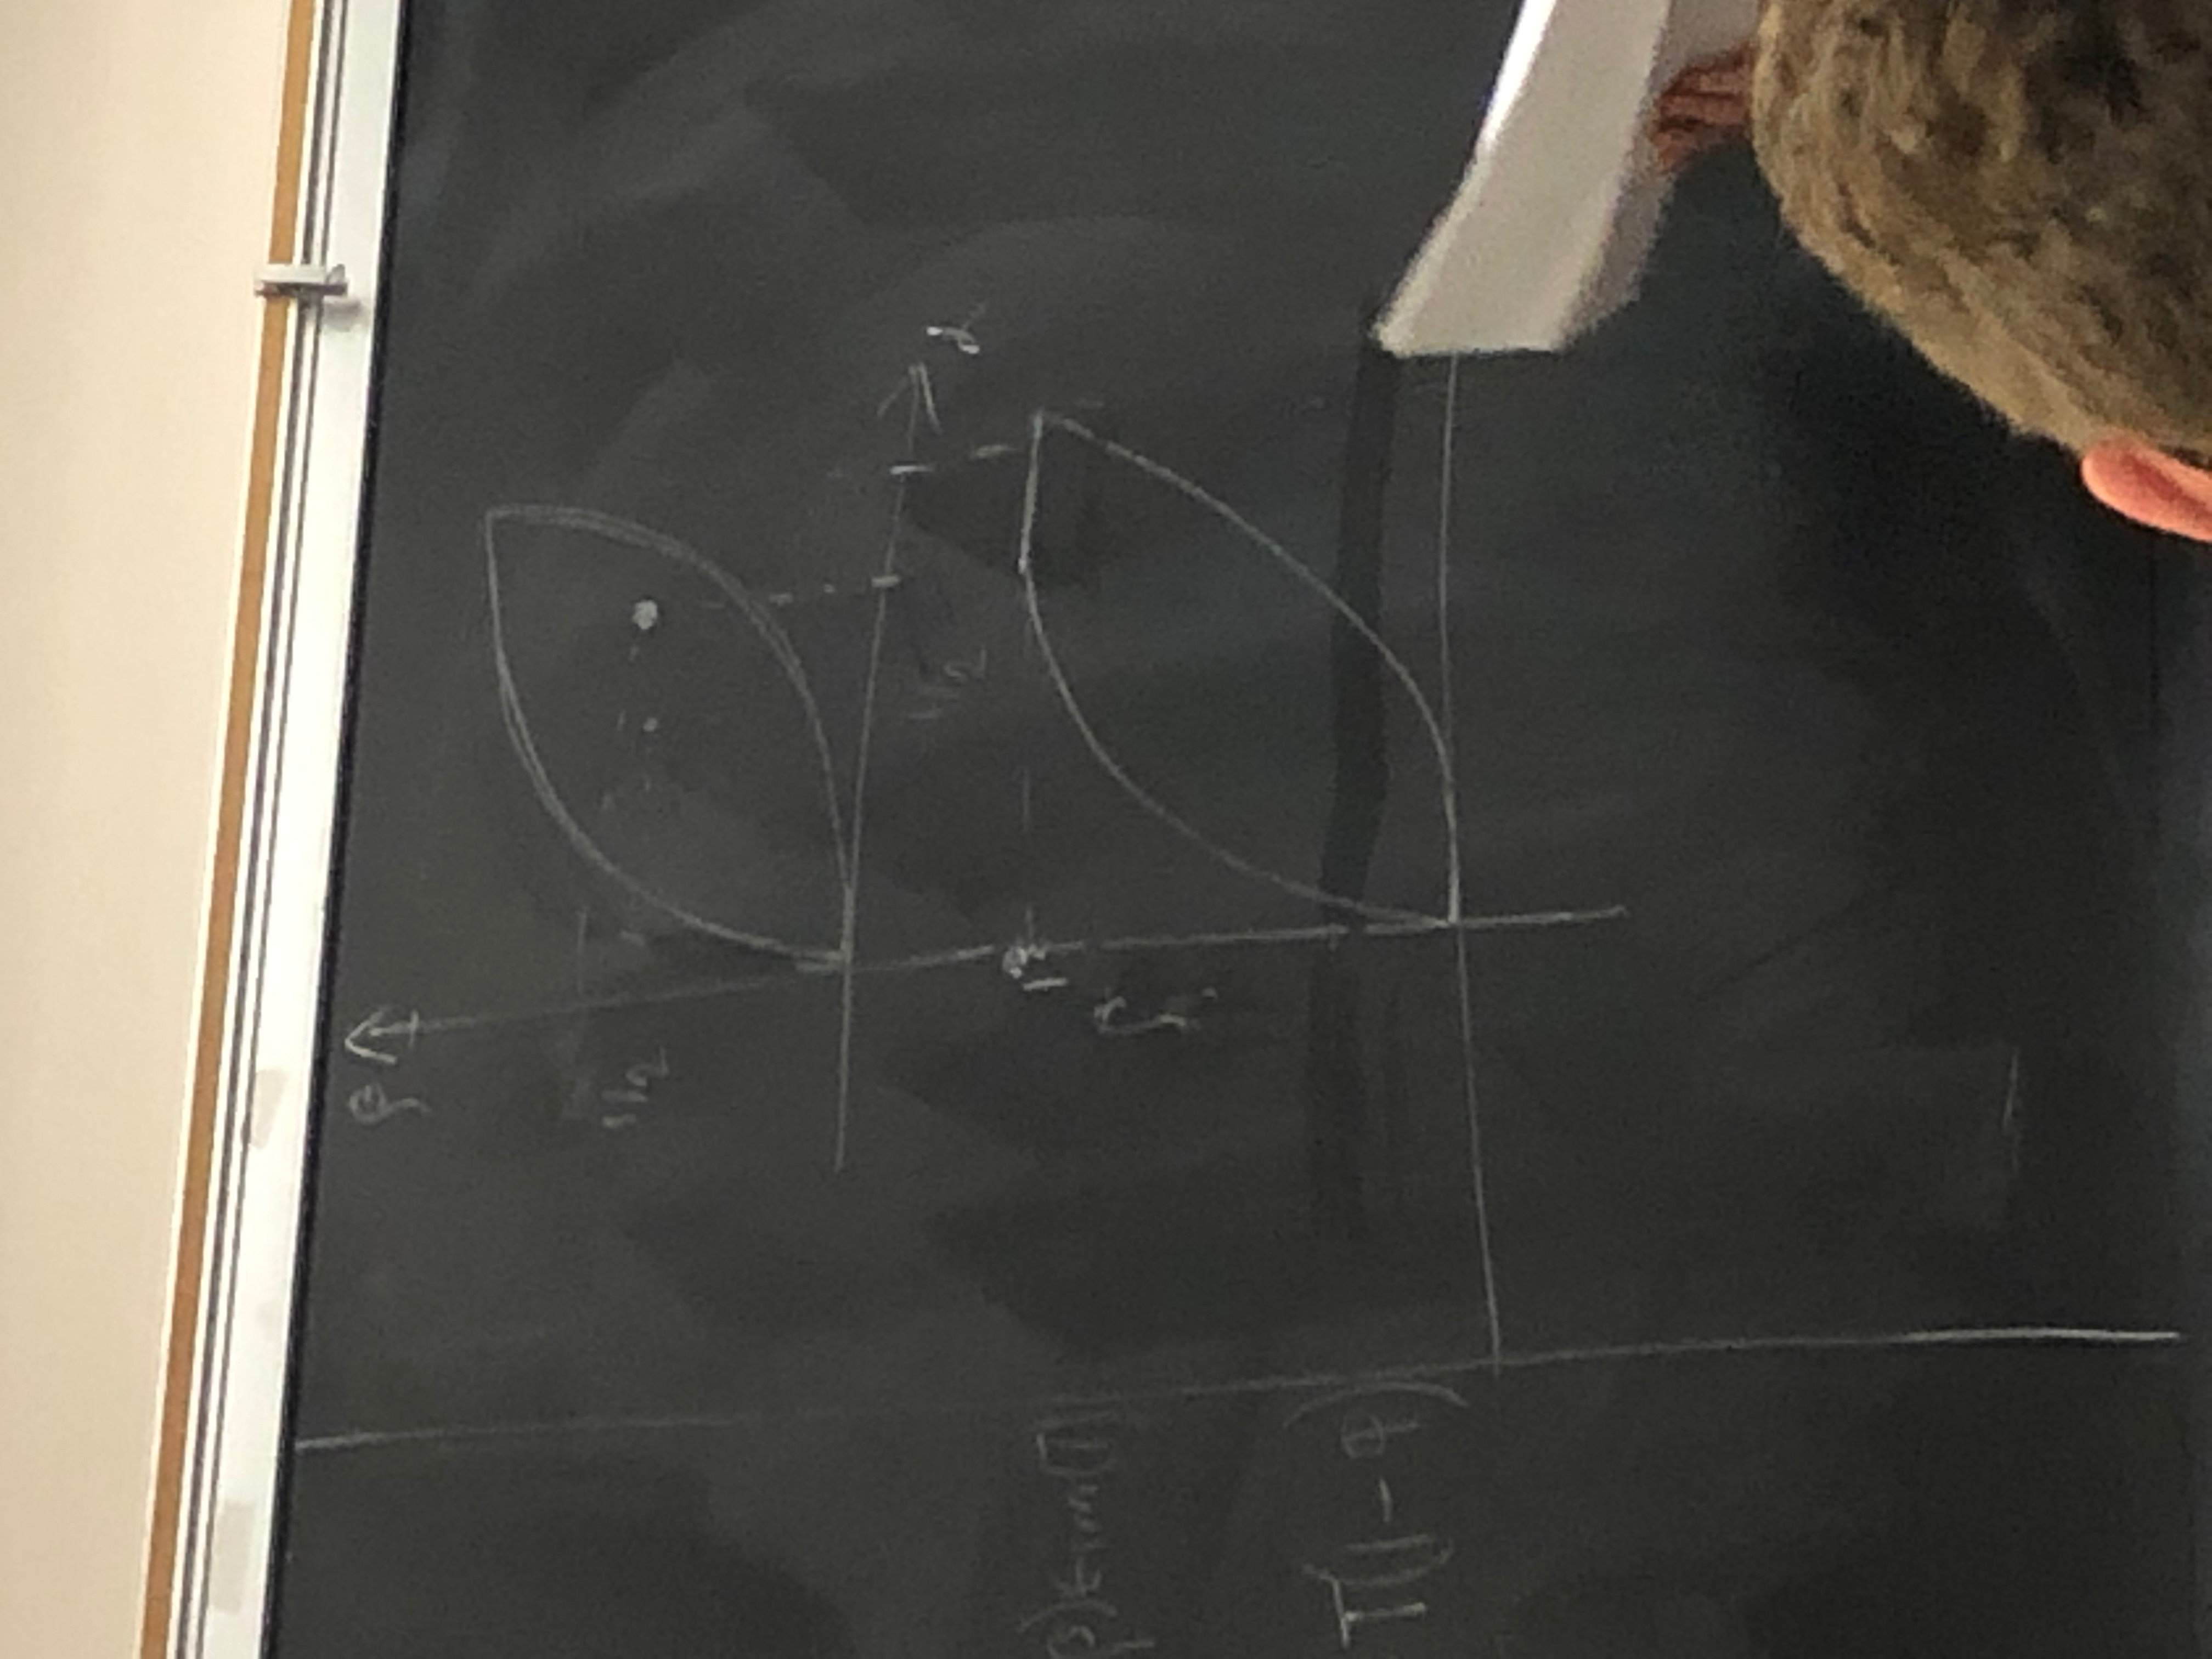
\includegraphics[scale=0.1, angle=270]{mathstats_np_set}
\caption{Sets of possible Neyman-Pearson tests; similar to Figure 3.1 in Lehmann and Romano.}
\label{mathstats.fig.np.sets}
\end{center}
\end{figure}

\begin{exercise}

\begin{enumerate}

\item Let \(\phi^*\) be the MP test of size \(\alpha\). Then \(\beta_{\phi^*} \geq \alpha\). Moreover, \(\beta_{\phi^*}\) is strictly greater than \(\alpha\) unless \(P = Q\) (Use N-P lemma, part 1). 

\item Let \(X_1, \ldots, X_n\) be i.i.d. uniform. \(H_0: X_1, \ldots, X_n \sim \operatorname{U}(0,1)\). \(H_a: X_1, \ldots, X_n \sim U(1/3, 2/3)\). Derive a UMP test of size \(\alpha\) for all values of \(\alpha\).

\end{enumerate}

\end{exercise}

\begin{solution}

\begin{enumerate}

\item

\item

\[
q(x_1, \ldots, x_n) = e^n  \prod_{i=1}^n I \{x_i \in [1/3, 2/3] ]\} = e^n I \{x_1, \ldots, x_n \in [1/3, 2/3]\}
\]

Similarly,

\[
p(x_1, \ldots, x_n) = I \{x_1, \ldots, x_n \in [0,1]\}.
\]

Note that the ratio \(q/p\) only takes on three values. By the Neyman-Pearson Lemma, the most powerful test \(\phi^*\) is either

\[
\phi_1^*(x_1, \ldots, x_n) = \begin{cases}
1, & q(x_1, \ldots, x_n)/p(x_1, \ldots, x_n) = 3^n  \\
\gamma, & q(x_1, \ldots, x_n) /p(x_1, \ldots, x_n) = 0 
\end{cases}
\]

or

\[
\phi_2^*(x_1, \ldots, x_n) = \begin{cases}
\gamma, & q(x_1, \ldots, x_n)/p(x_1, \ldots, x_n) = 3^n  \\
0, & q(x_1, \ldots, x_n) /p(x_1, \ldots, x_n) = 0 
\end{cases}
\]

Now

\[
\alpha_{\phi_1^*} = \E_P \phi_1^* (X_1, \ldots, X_n) = 1 \cdot \mathbb{P}(X_1, \ldots, X_n \in [1/3, 2/3]) + \gamma \mathbb{P}(\text{at least one } X_j \text{ is outside } [1/3, 2/3])
\]

\[
= 3^{-n} + \gamma(1 - 3^{-n}) = \alpha 
\]

which has a solution for \(\gamma(\alpha)\) for \(\alpha \geq 3^{-n}\). On the other hand,

\[
\alpha_{\phi_2^*} = \E_P \phi_2^* (X_1, \ldots, X_n) = \gamma \mathbb{P}(X_1, \ldots, X_n \in [1/3, 2/3]) + 0 \cdot \mathbb{P}(\text{at least one } X_j \text{ is outside } [1/3, 2/3])
\]

\[
= \gamma 3^{-n} = \alpha
\]

which has a unique solution \(\gamma(\alpha)\) for \(\alpha \leq 3^{-n}\). So for a test with a very small \(\alpha\), you need to consider a strictly randomized test like \(\alpha_{\phi_2^*}\). 

\end{enumerate}

\end{solution}


\begin{theorem}[\textbf{Went over last time}]

We have a sequence \(X_1, \ldots, X_n\) distributed i.i.d. Last time we showed that the following hypothesis testing problem:

\[
H_0: X_1, \ldots, X_n \sim P, \qquad H_A: X_1, \ldots, X_n \sim Q
\]

with

\[
\frac{dP}{d\mu} = p, \qquad \frac{dQ}{d\mu} = q
\]

using the test

\begin{equation}\label{mathstats.np.test.def}
\phi^* (x_1, \ldots, x_n) = \begin{cases}
1, &  \prod_{i=1}^n q(x_i) > c \prod_{i=1}^n p(x_i) \\
\gamma ,&   \prod_{i=1}^n q(x_i) =  c \prod_{i=1}^n p(x_i)  \\
0, &  \prod_{i=1}^n q(x_i) <  c \prod_{i=1}^n p(x_i) 
\end{cases}
\end{equation}

is UMP of size \(\alpha = \E_P(\phi^*)(X_1, \ldots, X_n)\) (given the correct choice of \(\gamma\)).

\end{theorem}

\begin{remark}

Intuition: if the likelihood function for \(Q\) exceeds the likelihood function of \(P\) by a reasonable amount (determined by \(c\)), choose \(Q\) to be more likely than \(P\).

Also, \(\phi^*\) of this kind is referred to as a \textit{Neyman-Pearson test.}

\end{remark}

%######################
\subsubsection{Consistency of Neyman-Pearson Tests}
%######################

We want the test to be consistent---as we collect more data and \(n \to \infty\), errors of both types go to 0. We hope to show the consistency of Neyman-Pearson tests.

\begin{definition}[\textbf{Consistency of a hypothesis test}]

Consider the framework of the Neyman-Pearson lemma (described above). A sequence of tests \(\{\phi_n\}_{n \geq 1}\), where \(\phi_n = \phi_n(x_1, \ldots, x_n)\) is \textit{consistent} if and only if

\[
\alpha_{\phi_n} = \E_P \phi_n(X_1, \ldots, X_n) \to 0, \qquad \text{and } \beta_{\phi_n} = \E_Q \phi_n(X_1, \ldots, X_n) \to 1 \qquad \text{as } n \to \infty.
\]

\end{definition}

It turns out that \(c\) grows with \(n\), and the growth condition of the size of this \(c_n\) is related to a measure of distance between \(P\) and \(Q\) (Hellinger distance). 

Recall the following definition:

\begin{definition}[\textbf{Hellinger Distance and Affinity (see Section 13.1 of Lehmann and Romano)}]

The \textit{Hellinger distance} between probability laws \(P\) and \(Q\) is defined as 

\[
H^2(P,Q) := \int_S (\sqrt{p} - \sqrt{q})^2 \ d\mu = 2 \int_S (1 - \sqrt{pq}) d \mu = 2 - 2 \int_@ \sqrt{pq} \ d\mu.
\]

Further,

\[
A(P,Q) := \int \sqrt{pq} \ d\mu
\]

is known as the \textit{Hellinger affinity.} 

%It satisfies a nice property: if one takes the distances the distributions of two random variables \(X_1, Y_1\), \(X_2, Y_2\), \ldots, \(X_n, Y_n\), 

\end{definition}

\begin{remark}

This is a true distance---it satisfies the Triangle Inequality, \(H(P,Q) = 0\) if and only if \(P = Q\) almost everywhere.

\end{remark}

\begin{lemma}

Let \(X \sim P\) and \(Y \sim Q\). Let \(X_1, \ldots, X_n\) be i.i.d. copies of \(X\) and likewise for \(Y_1, \ldots, Y_n\), so \((X_1, \ldots, X_n) \sim P^n\) and \((Y_1, \ldots, Y_n) \sim Q^n\). Then

\[
A(P^n, Q^n) =  \left[ A(P, Q) \right]^n.
\]

\end{lemma}

\begin{proof}

%\begin{multline*}
%A(P^n, Q^n) = \int \sqrt{p(x_1, \ldots, x_n)} \sqrt{ q( x_1, \ldots, x_n) } \ d\mu \\
%= \prod_{j=1}^n \int \sqrt{p(x_i) q(x_i) \ d\mu
%\end{multline*}

\[
A(P^n, Q^n) = \int \sqrt{p(x_1, \ldots, x_n)} \sqrt{ q( x_1, \ldots, x_n) } \ d\mu^n 
= \prod_{j=1}^n \int \sqrt{p(x_j) q(x_j)} \ d\mu=  \left[ A(P, Q) \right]^n.
\]

\end{proof}

\begin{theorem}[\textbf{Consistency of Neyman-Pearson tests}]

Assume that \(\rho := A(P,Q) < 1\). Then take any sequence \(\{c_n\} \subset \mathbb{R}_+\) such that 

\begin{equation}\label{mathstats.cons.np.a}
\rho^{2n} \ll c_n \ll \rho^{-2n}.
\end{equation}

Then any sequence \(\{\phi_n\}_{n \geq 1}\) of Neyman-Pearson tests corresponding to \(\{c_n\}_{n \geq 1}\) is consistent. 

\end{theorem}

\begin{proof}

First, we will show that \(\alpha_{\phi_n} \to 0\) under these conditions. Recall the definition of \(\phi\) from (\ref{mathstats.np.test.def}). 

\begin{multline*}
\alpha_{\phi_n}  = \int \phi(x_1, \ldots, x_n) p(x_1, \ldots, x_n) \ d \mu^n \\
\leq \int I  \left\{  \frac{ \prod_{i=1}^n q(x_i)}{ \prod_{i=1}^n p(x_i)} \geq c_n \right\} p(x_1) \cdots p(x_n)  \ d\mu^n \\
\leq \int  \sqrt{\frac{ q(x_1) \cdots q(x_n)}{c_n p(x_1) \cdots p(x_n) } }  p(x_1) \cdots p(x_n) \ d \mu^n \\
= \frac{1}{\sqrt{c_n}} \int \sqrt{q(x_1) \cdots q(x_n)} \sqrt{ p(x_1) \cdots p(x_n)} d \mu^n = \rho^n c_n^{-1/2}  \to 0 \text{ as } n \to \infty.
\end{multline*}



(The second inequality follows because when the indicator equals 0 the square root term is greater than or equal to 0 but when the indicator equals 1 the square root term is greater than or equal to 1. The last step follows by assumption of the lemma.)

Now consider the Type II error \(1 - \beta_{\phi_n}\). 

\begin{multline*}
1 - \beta_{\phi_n} = \int [1 - \phi(x_1, \ldots, x_n)]q(x_1) \cdots q(x_n) \ d\mu^n \\
\leq \int I \left\{q(x_1) \cdots q(x_n) \leq c p(x_1) \cdots p(x_n) \right\} q(x_1) \cdots q(x_n) \ d\mu^n \\
\leq  \int  \sqrt{\frac{ p(x_1) \cdots p(x_n)}{q(x_1) \cdots q(x_n) }  \cdot c_n  }  \cdot q(x_1) \cdots q(x_n) \ d \mu^n  \\
= \sqrt{c_n} A(P^n, Q^n) = c-n^{1/2} \rho^n \to 0 \text{ as } n \to \infty
\end{multline*}

\end{proof}

\begin{remark}

Intuition: \( A(P,Q) < 1 \iff  H(P, Q) > 0 \iff P \neq Q\). Also, \(a_n \ll b_n \iff a_n = o(b_n)\), and \(a_n \gg b_n \iff b_n \ll a_n\). Almost all reasonable sequences satisfy (\ref{mathstats.cons.np.a})---this range is very large. 

Basically, this theorem says the Type I and Type II errors converge to 0 geometrically fast (as \(\rho^n\)) if \(P\) and \(Q\) are not too close together.

\end{remark}

%######################
\subsubsection{Composite Hypothesis Testing}
%######################

% !!Please put ########## above and below the section/subsection name for better readability (as the section name above)

% Some comments regarding LaTeX typesetting:
% (1) Please use \[ math here  \] instead of $$ math here $$ for displayed equations, and separate them from the main text: 
% for example, 
% \[
% \sqrt{x^2} = | x |
% \]
% (2) Please use \begin{multline} \end{multline} for numbered multiline equations, or \begin{multline*} \end{multline*} for non-numbered equations ( \\ symbol is used for line breaks), and \begin{equation} \end{equation} for numbered one-line equations
% (3) use \l and \r (shortcuts for \left and \right) for automatic bracket resizing, for example 
% $\l( \int\limits_0^\infty f(x) dx \r)^2 \leq \int\limits_0^infty f^2(x) dx$
% To make the code readable, try to keep lines short (by pressing "enter" in your editor). 


We will start with one-dimensional family (one parameter), then expand to multiple parameters using tricks based on conditioning and using the principles of sufficiency and completeness.

\begin{definition}[\textbf{Composite Hypothesis Test}]



Assume we have a statistical model \(\{P_\theta, \theta \in \Theta\}\). Let \(\Theta_0, \Theta_1 \subset \Theta\) be such that \(\Theta_0 \cap \Theta_1 = \emptyset\) and \(\Theta_0 \cup \Theta_1 = \Theta\). Assume \( X \sim P_\theta \text{ for some } \theta \in \Theta\) (where \(X\) may be multivariate). We would like to test the hypotheses

\[
H_0:  \theta \in \Theta_0, \qquad H_a: \theta \in \Theta_1.
\]

Such a test is a \textit{composite hypothesis test}.

\end{definition}

The Neyman-Pearson Lemma does not directly apply to composite hypothesis tests, but it turns out we can use the Neyman-Pearson lemma to prove some results about some composite hypothesis tests under some circumstances.

\begin{definition}[\textbf{Power function; definition 8.3.1 in Casella and Berger}]

The \textit{power function} of a test \(\phi\) is defined as

\[
\beta_\phi(\theta) := \E_\theta \phi(X).
\]

\end{definition}

\begin{remark}

For \(\theta \in \Theta_0\), \(\beta_\phi(\theta)\) is the probability of a Type 1 error; for \(\theta \in \Theta_1\), \(\beta_\phi(\theta)\) is the power of \(\phi\).

\end{remark}

\begin{definition}[\textbf{Test size; definition 8.3.6 in Casella and Berger}]

The test \(\phi\) is of \textit{size} \(\alpha\) if and only if 

\[
\sup_{\theta \in \Theta_0} \beta_\phi(\theta) \leq \alpha.
\]

\end{definition}

\begin{definition}[\textbf{Uniformly most powerful test; definition 8.3.11 in Casella and Berger}]

\(\phi^*\) is the \textit{uniformly most powerful test} of size \(\alpha\) if \(\phi^*\) is of size \(\alpha\) and \(\beta_{\phi^*}(\theta) \geq \beta_\phi(\theta)\) for any other test \(\phi\) of size \(\alpha\) for all \(\theta \in \Theta_1\).

\end{definition}

We will be interested in families with \textit{monotone likelihood ratios}. (Note: for the rest of the class today, \(\Theta = [a, b] \subseteq \mathbb{R}\) with \(a, b \in [-\infty, \infty]\)). 

\begin{definition}[\textbf{Monotone likelihood ratio; definition 8.3.16 in Casella and Berger}]

Let \(T(X)\) be a statistic. Consider \(\Theta \subseteq \mathbb{R}\) as a segment on the real line. We say that the family of pdfs \(\{p_\theta, \theta \in \Theta\}\) has a \textit{monotone likelihood ratio (MLR)} with respect to \(T(x)\) if and only if for any \(\theta' > \theta''\), 

\[
\frac{p_{\theta'}(x)}{p_{\theta''}(x)} = \psi_{\theta', \theta''}(T(x))
\]

where \(\psi_{\theta', \theta''}(\cdot)\) is non-decreasing. (That it is non-decreasing is without loss of generality; in the case that \(\psi\) is non-increasing, simply replace \(T(x)\) with \(-T(x)\) to achieve a non-decreasing \(\psi\)).

\end{definition}

\begin{example}

Let \(X \sim \operatorname{Poisson}(\lambda)\), so 

\[
p_\lambda(x) =  \frac{e^{-\lambda} \lambda^x}{x!}, \qquad x \in \mathbb{Z}_+.
\]

Then  \(\{ \operatorname{Poisson}(\lambda), \lambda \in \mathbb{R}_+\}\) has a monotone likelihood ratio with respect to \(T(x) =x\) by the following argument. Take \(\lambda' > \lambda ''\). Then 

\[
\frac{e^{- \lambda '} (\lambda')^x x! }{x! e^{-\lambda ''} (\lambda'')^x }=  e^{-(\lambda' - \lambda'')} \left( \frac{ \lambda'}{\lambda ''} \right)^x
\]

and

\[
\psi_{\lambda', \lambda''}(x) = e^{-(\lambda' - \lambda'')} \left( \frac{ \lambda'}{\lambda ''} \right)^x
\]

is non-decreasing. 

\end{example}

\begin{theorem}[\textbf{Karlin-Rubin; similar to Theorem 8.3.17 in Casella and Berger, Theorem 3.4.1 in Lehmann and Romano}]\label{mathstasts.thm.karlin.rubin}

Assume \(\{p_\theta, \theta \in[a,b]\}\) has a monotone likelihood ratio with respect to some \(T(x)\). Suppose we want to test

\[
H_0: \theta \leq \theta_0, \qquad H_a: \theta > \theta_0.
\]

Then there exists \(c \geq 0\) and \(\gamma \in [0,1]\) such that 

\[
\phi^*(x) = \begin{cases}
1, &  T(x) >c \\
\gamma, & T(x) = c \\
0, & T(x) < c
\end{cases}
\]

is the uniformly most powerful test of size \(\alpha\). (In other words, the UMP test will always be of this form.)

\end{theorem}

\begin{proof}

We will show that this is the uniformly most powerful test over the larger family of tests that satisfy \(\E_{\theta_0} \phi(x) = \alpha\) (\(\beta_\phi(\theta_0) \leq \alpha\)), which contains tests of size \(\alpha\). So if we can find the UMP test for this larger family (and it is a test of size \(\alpha\)), then that is also the UMP test for test of size \(\alpha\) (satisfying \(\sup_{\theta \in \Theta_0} \beta_\phi(\theta) \leq \alpha\)).

First note that we can always find \(c\) and \(\gamma\) such that 

\[
\E_{\theta_0}(\phi^*(x) = \alpha.
\]

Define \(F(c) := \mathbb{P}_{\theta_0}( \{x: T(x) \leq x\})\). Note that

\[
\E_{\theta_0}\psi^*(x) = F(c) + \gamma[F(c) - F(c^+)]
\]

where \(F(c) - F(c^+)\) is the size of the jump. (The proof of this claim is an exercise.) 

Next, take \(\theta' > \theta_0\) and consider the simple hypothesis test

\[
H_{0}': \theta = \theta_0, \qquad H_a': \theta = \theta'.
\]

By the Neyman-Pearson Lemma, the most powerful test for this is 

\[
\phi'(x) = \begin{cases}
1, & p_{\theta'}(x) > c' p_{\theta_0}(x) \\
\gamma', &  p_{\theta'}(x) = c' p_{\theta_0}(x) \\
0, & p_{\theta'}(x) < c' p_{\theta_0}(x) 
\end{cases} \iff 
\phi'(x) = \begin{cases}
1, & p_{\theta'}(x)/  p_{\theta_0}(x) > c' \\
\gamma', &  p_{\theta'}(x)/  p_{\theta_0}(x) = c' \\
0, & p_{\theta'}(x)/ p_{\theta_0}(x)  < c' 
\end{cases}
\]

But since \( p_{\theta'}(x)/  p_{\theta_0}(x)  = \psi(T(x))\), by the assumption of the monotone likelihood ratio property,

\[
\frac{p_{\theta'}(x)}{  p_{\theta_0}(x)} > c' \iff T(x) > \psi^{-1}(c').
\]

Set \(\psi^{-1}(c') = c\) and \(\psi^{-1}(\gamma') = \gamma\) (using the values of \(\gamma\) and \(c\) from earlier in the proof). Then we have

\[
\phi'(x) = \begin{cases}
1, & T(x) > c \\
\gamma', & T(x) = c \\
0, & T(x) < c
\end{cases}
\]

as desired. (Moreover, \(c\) and \(\gamma\) are uniquely determined by \(\E_{\theta_0}(\phi^*) = \alpha\). Note that \(\theta'\) does not appear anywhere in this test. Since \(\theta'\) was arbitrary, the proof is almost complete.

The final argument is to show that this test has size \(\alpha\). Namely, we must show

\[
\sup_{\theta \leq \theta_0} \beta_{\phi^*}(\theta) = \sup_{\theta \leq \theta_0} \E_\theta \phi^*(x) \leq \alpha.
\]

It is sufficient to show that \(\beta_{\phi^*}(\theta)\) is monotone. Take \(\theta_1 < \theta_2\). Then by the Neyman-Pearson Lemma, we know that \(\phi^*\) is the UMP test for testing

\[
H_0'':  \theta = \theta_1 \qquad H_a'':  \theta = \theta_2
\]

of size \(\beta_{\phi^*}(\theta)\). Since it is the most powerful test, its power \(\E_{\theta_2} \phi^*(x)\) is at least as powerful than the test which is identically equal to \(\beta_{\phi^*}(\theta)\); that is, \(\E_{\theta_2}(\phi^*(x) \geq \E_{\theta_1}(\phi^**(x)\).

%this will be done in the next lecture. From there we can conclude that this is the uniformly most powerful test of size \(\alpha\).


\end{proof}


\begin{example}

\(X_1, \ldots, X_n \sim \mathcal{N}(\mu, 1)\). Test \(H_0: \mu \leq 0\) against \(H_1: \mu > 0\). Find the UMP test.

\end{example}

\begin{solution}

Take \(\mu_1 > \mu_2\). Then 

\begin{multline*}
\frac{ p_{\mu_1}(x_1, \ldots, x_n)}{ p_{\mu_2}(x_1, \ldots, x_n)} = \exp \left\{ - \frac{1}{2} \left[ \sum_{i=1}^n (x_i - \mu_1)^2 -  \sum_{i=1}^n (x_i - \mu_2)^2  \right]\right\}
\\ = \exp \left\{ - \frac{1}{2} \left[ n(\mu_1^2 - \mu_2^2) + (\mu_1 - \mu_2) \sum_{i=1}^n x_i \right]\right\}
\end{multline*} 

This is an increasing function with respect to \(T(x_1, \ldots, x_n) = \sum_{i=1}^n x_i\). Therefore by Theorem \ref{mathstasts.thm.karlin.rubin}, we have that the UMP test is 

\begin{equation}\label{mathstats.kr.ex.1}
\phi(x_1, \ldots, x_n) = \begin{cases}
1, & \sum_{i=1}^n x_i \geq c_\alpha \\
0, & \sum_{i=1}^n x_i < c_\alpha
\end{cases} = \begin{cases}
1, & n^{-1/2} \sum_{i=1}^n x_i \geq c_\alpha' \\
0, & n^{-1/2} \sum_{i=1}^n x_i < c_\alpha'
\end{cases}
\end{equation}

Note that 

\[
\E_{\mu=0} \phi(X_1, \ldots, X_n) = \alpha \iff  \mathbb{P} \left( \frac{1}{\sqrt{n}} \sum_{i=1}^n X_i \geq c_\alpha' \right) = \alpha
\]

and \(n^{-1/2} \sum_{i=1}^n X_i  \sim \mathcal{N}(0,1)\). Therefore \(c_\alpha' = z_{1- \alpha}\) (the \(1-\alpha\) quantile of a standard Gaussian distribution). Substituting this into (\ref{mathstats.kr.ex.1}) defines the UMP test.

\end{solution}

\begin{remark}

The Karlin-Rubin Theorem (Theorem \ref{mathstasts.thm.karlin.rubin}) still applies if the inequalities in the hypothesis test are reversed.

\end{remark}

\begin{example}

\(X_1, \ldots, X_n \sim \mathcal{N}(\mu, 1)\). Test \(H_0: \mu \in [0,1]\) against \(H_1: \mu < 0 \cup \mu > 1\). Does there exist a UMP test?

\end{example}

\begin{solution}

No. Consider \(H_0': \mu \in [0,1], H_a': \mu > 1\) and \(H_0'': \mu \in [0,1], H_a'': \mu < 1\). If the UMP test for our test exists, it must be identical to the UMP tests for both of these tests (since it would have to be UMP over ever \(\theta\)). By Theorem \ref{mathstasts.thm.karlin.rubin}, the UMP test in the first case is 

\[
\phi'(x_1, \ldots, x_n) = \begin{cases}
1, & \sum_{i=1}^n x_i \geq c \\
0, & \sum_{i=1}^n x_i < c.
\end{cases}
\]

The UMP test in the second case is 

\[
\phi'(x_1, \ldots, x_n) = \begin{cases}
1, & \sum_{i=1}^n x_i \leq c \\
0, & \sum_{i=1}^n x_i > c.
\end{cases}
\]

Since these tests are not identical, there is no UMP test for our test.

\end{solution}

\begin{theorem}[\textbf{Generalized Neyman-Pearson Lemma, Theorem 3.6.1 in Lehmann and Romano}]

Assume that \(f_0, f_1, \ldots, f_n: \mathbb{R}^d \to \mathbb{R}\) such that 

\[
\int |f_j| \ d\mu < \infty, \qquad j \in \{0, \ldots, N\}.
\]

\begin{enumerate}

\item

We seek to maximize the \(\int \phi  f_0 \ d\mu \) over all tests \(\phi\) subject to \(\int \phi f_j \ d\mu = \alpha_j, j \in \{1, \ldots, N\}\). 

\item

We seek to maximize the \(\int \phi  f_0 \ d\mu \) over all tests \(\phi\) subject to \(\int \phi f_j \ d\mu \leq \alpha_j, j \in \{1, \ldots, N\}\). 

\end{enumerate}

Suppose there exists \(k_1, \ldots, k_N\) such that 

\[
\phi^* = \begin{cases}
1, & f_0(x) > k_1 f_1(x) + \ldots + k_N f_N(x) \\
0, & f_0(x) < k_1 f_1(x) + \ldots + k_N f_N(x) 
\end{cases}
\]

satisfies \(\int \phi^* f_j \ d\mu = \alpha_j, j \in \{1, \ldots, N\} \). Then \(\phi^*\) solves the first problem. Moreover, if \(k_1, \ldots, k_N \geq 0\), then \(\phi^*\) also solves the second problem.

\end{theorem}

\begin{example}[\textbf{Like Theorem 3.7.1 in Lehmann and Romano}]\label{mathstats.gnp.ex.prob}

\(\{P_\theta, \theta \in \Theta\}\). \(H_0: \theta \in [\theta_1, \theta_2]\). \(H_a: \theta \notin [\theta_1, \theta_2]\). We have 

\[
p_\theta(x) =  \frac{1}{c(\theta)} e^{\theta T(x)}
\]

(one-parameter exponential family). Find the UMP unbiased test.

\end{example}

\begin{solution}

For the test to be unbiased, the Type I error rate has to be less than or equal to \(\alpha\) (for all \(\theta \in [\theta_1, \theta_2]\)) and the power has to be greater than or equal to \(\alpha\) (for all \(\theta\) in the rejection region). We will use the Generalized Neyman-Pearson Lemma to show the solution is of the form

\[
\phi^*(x) = \begin{cases}
1, & T(x) < c_1 \text{ or } T(x) > c_2 \\
\gamma_1, & T(x) = c_1 \\
\gamma_2, & T(x) = c_2 \\
0, & T(x) \in (c_1, c_2)
\end{cases}
\]

such that \(\E_{\theta_1} \phi^*(X) = \E_{\theta_2} \phi^*(X) = \alpha\). By the Generalized Neyman-Pearson Lemma, we look for the solution in the form

\[
\tilde{\phi}(x) = \begin{cases}
1, & p_{\theta'}(x) > k_1  p_{\theta_1}(x) + k_2 p_{\theta_2}(x) \\
0, & p_{\theta'}(x) < k_1  p_{\theta_1}(x) + k_2 p_{\theta_2}(x).
\end{cases}
\]

This is equivalent to 

\begin{equation}\label{mathstats.np.gen.ex.a}
\tilde{\phi}(x) = \begin{cases}
1, & 1 > \tilde{k}_1e^{(\theta_1 - \theta') T(x)} + \tilde{k}_2e^{(\theta_2  - \theta') T(x)} \\
0, & 1 < \tilde{k}_1e^{(\theta_1 - \theta') T(x)} + \tilde{k}_2e^{(\theta_2  - \theta') T(x)}.
\end{cases}
\end{equation}

Let's analyze the inequality \(g(t) < 1\) where 

\[
g(t) =  \tilde{k}_1e^{a_1 t } + \tilde{k}_2e^{a_2 t}
\]

with \(a_1 = \theta_1 - \theta' > 0, a_2 = \theta_2 - \theta' > 0, a_1 < a_2\). Consider the second case.

\begin{enumerate}[(a)]

\item \(\tilde{k}_1 > 0, \tilde{k}_2 > 0 \implies g(t)\) is increasing. \(g(t) < 1 \iff t< c\) for some \(c \in \mathbb{R}\). From the Karlin-Rubin Theorem, in this case \(\beta_{\tilde{\phi}}(\theta) \) is monotone. But this is impossible, as \(\beta_{\tilde{\phi}}(\theta_1) =  \beta_{\tilde{\phi}}(\theta_2)\).

\item \(\tilde{k}_1 < 0, \tilde{k}_2 < 0 \implies g(t) < 1\). Examining (\ref{mathstats.np.gen.ex.a}) shows that in this case \(\tilde{\phi}(x) = 1\) for all \(x\) (so \(\tilde{\phi}\) always rejects), so we can't have controlled Type I error.

\item \(\tilde{k}_1 < 0, \tilde{k}_2 > 0\). In this case, \(g'(t) = \tilde{k}_1 a_1 e^{a_1 t} + \tilde{k}_2 a_2 e^{a_2 t}\). Then \(g'(t) = 0\) has a unique solution (see Figure \ref{mathstats_gnp_ex_fig}), and \(g(t) < 1 \iff t \in (c_1, c_2)\) (rejection only happens in this bounded interval). But this can't be a UMP unbiased test because the power function of this test is less than a constant test. We should have high power as our test statistic goes off to infinity or negative infinity, but examining (\ref{mathstats.np.gen.ex.a}), we see that \(\tilde{\phi}(x)= 0\) as \(T(x) \to \infty\) or \(- \infty\).

\begin{figure}[htbp]
\begin{center}
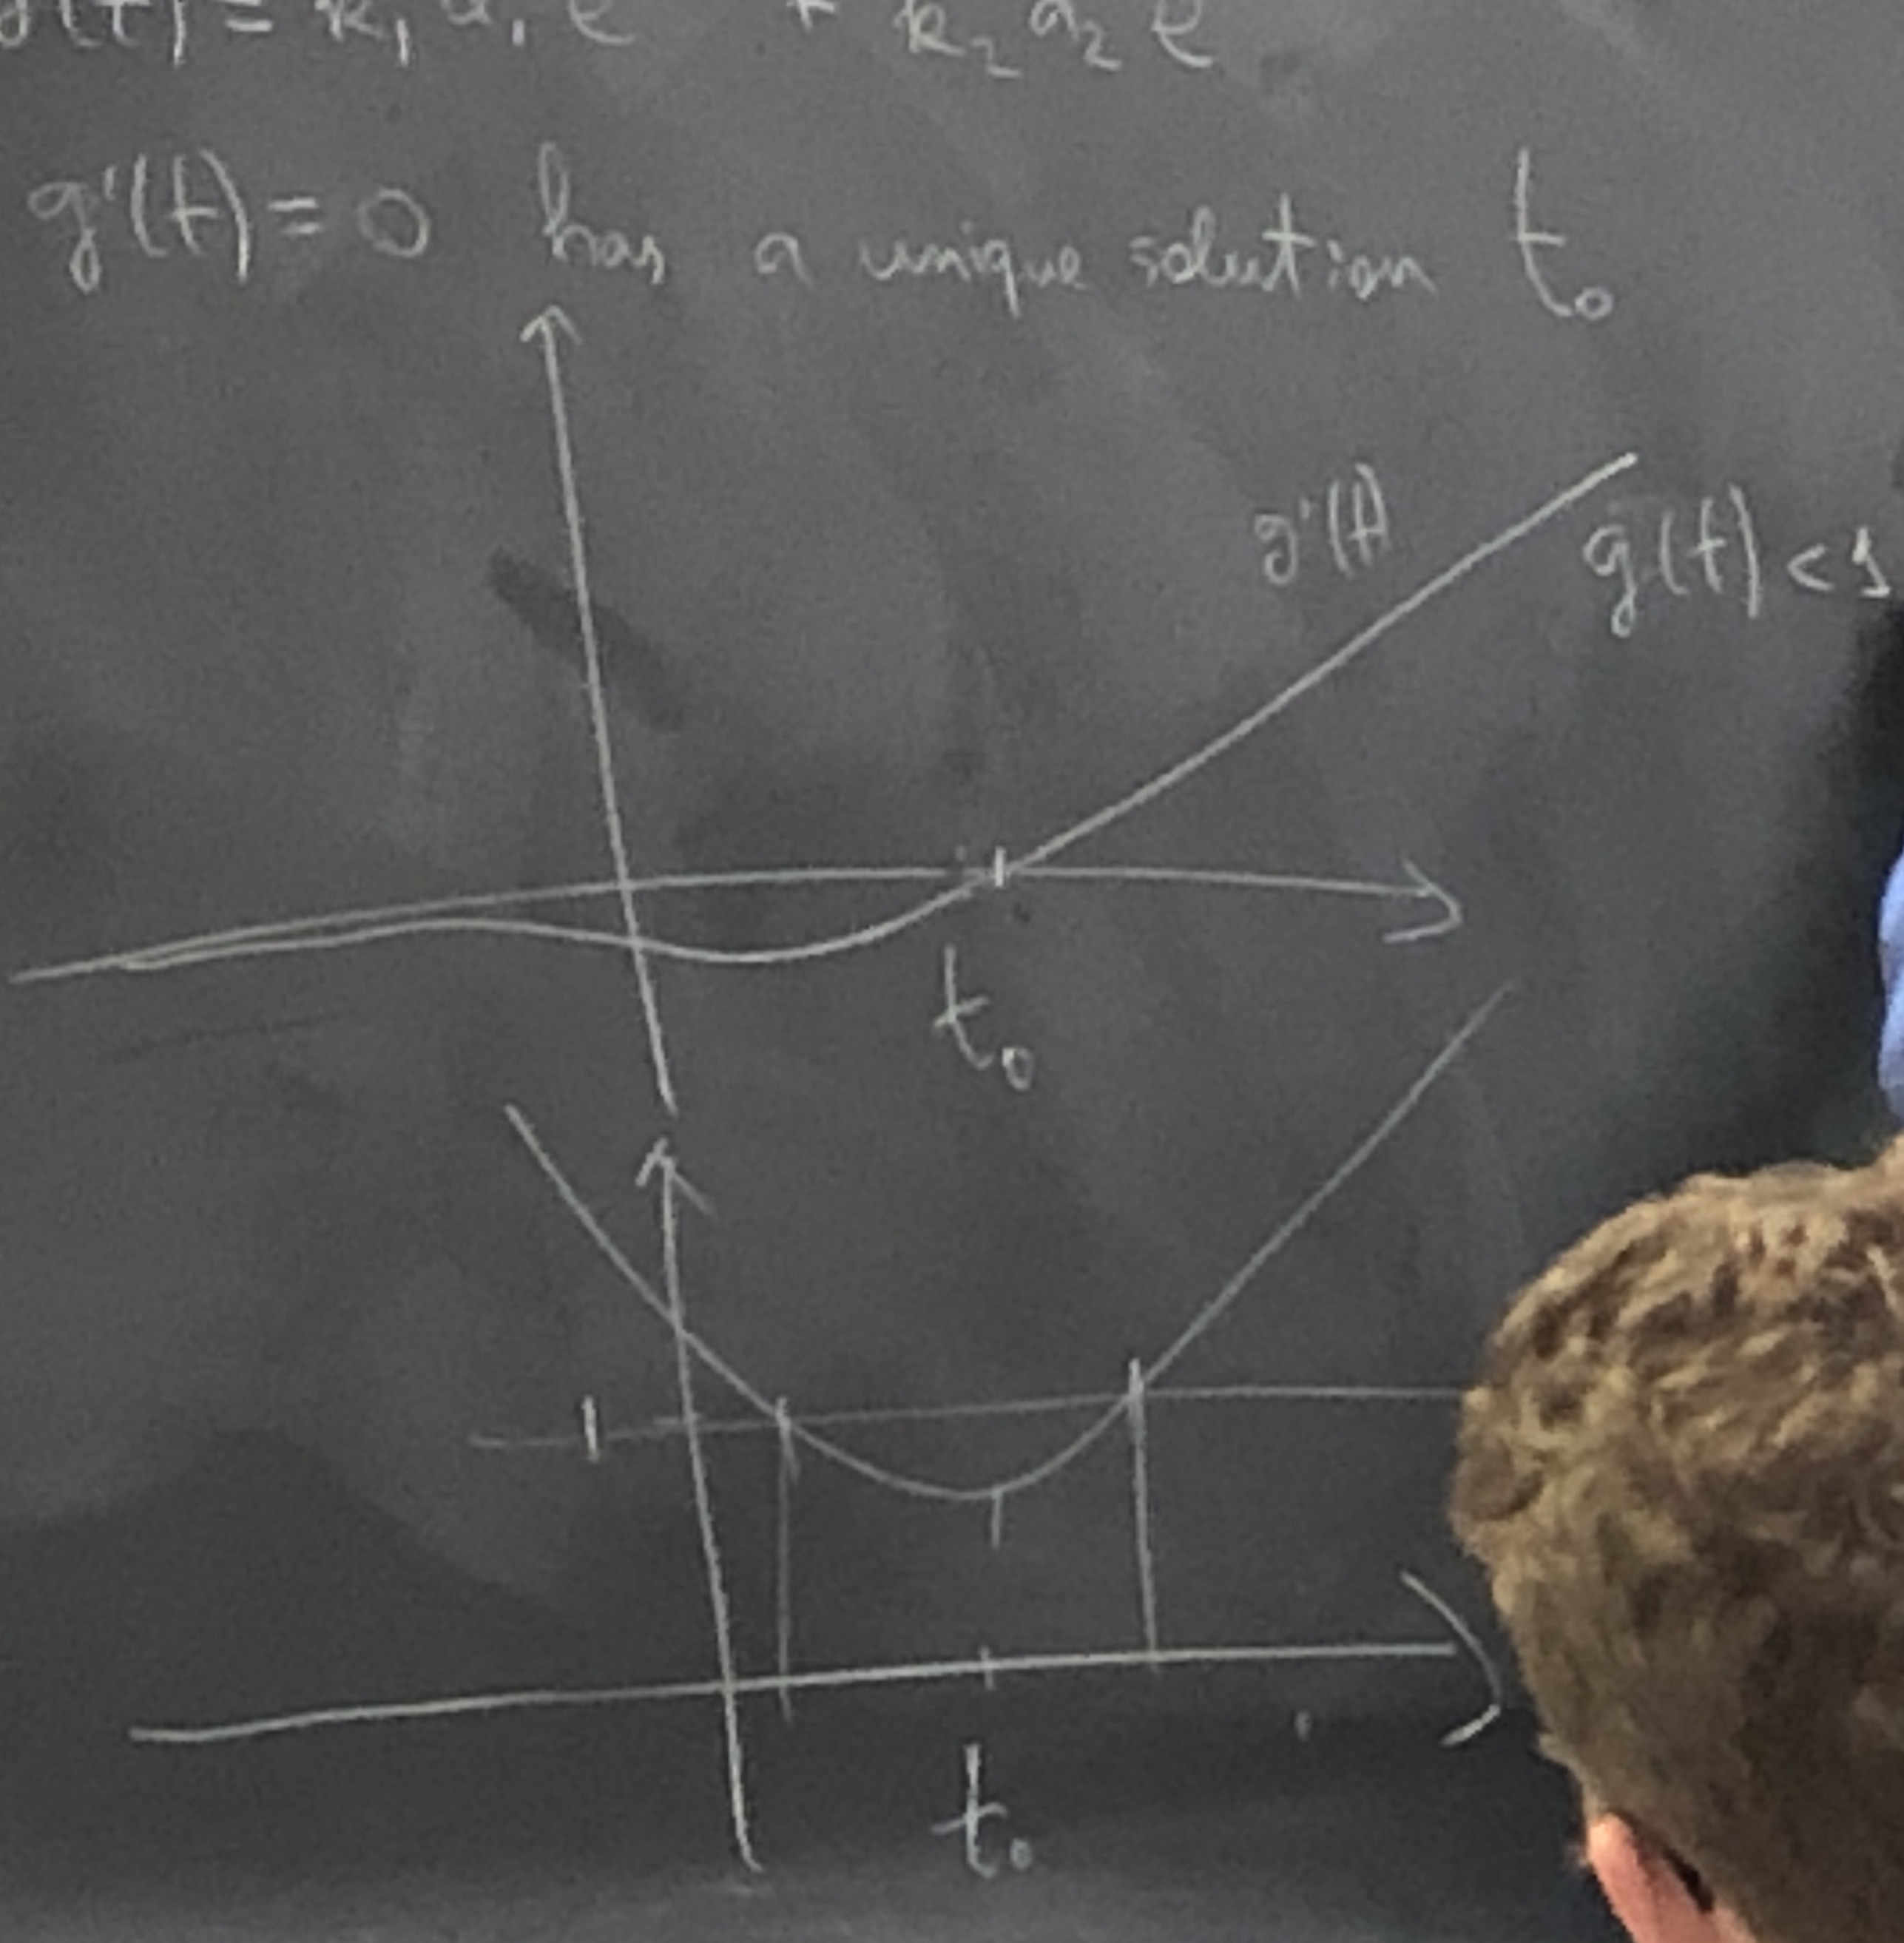
\includegraphics[scale=0.1]{mathstats_gnp_ex}
\caption{Figure for Example \ref{mathstats.gnp.ex.prob}, case (c). This can't be the UMP unbiased test because our power is approaches 0 the further away we get from this narrow interval (we accept the null hypothesis when this function is more than 1).}
\label{mathstats_gnp_ex_fig}
\end{center}
\end{figure}

\item \(\tilde{k}_1 > 0, \tilde{k}_2 < 0\). Then \(g'(t)\) has a unique zero (see Figure \ref{mathstats_gnp_ex_fig_2}), and \(g(t) < 1 \iff t \in (c_1, c_2)\) which gives us the form of the test that we were looking for (we always accept the null hypothesis when this function is more than 1 and reject it when it is less than 1).

\begin{figure}[htbp]
\begin{center}
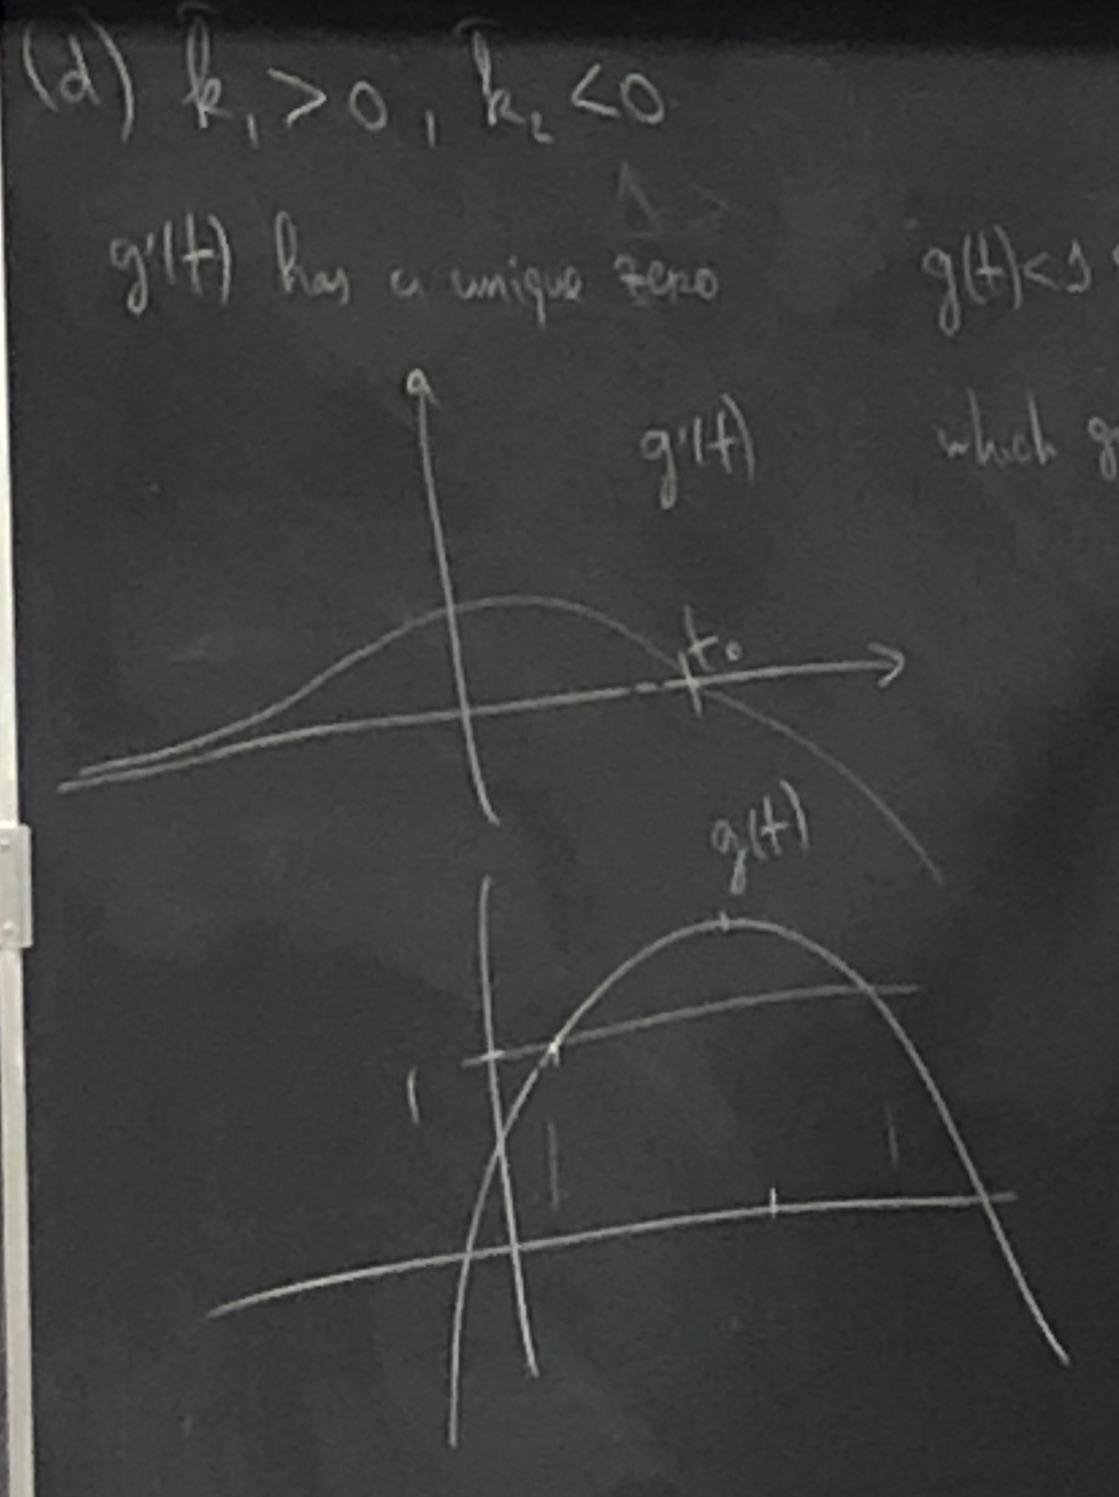
\includegraphics[scale=0.2]{mathstats_gnp_ex_2}
\caption{Second figure for Example \ref{mathstats.gnp.ex.prob}, case (d). This is the form of the UMP unbiased test.}
\label{mathstats_gnp_ex_fig_2}
\end{center}
\end{figure}


\end{enumerate}

It remains to show that \(\beta_{\phi^*}(\theta) \leq \alpha\) for all \(\theta \in [\theta_1, \theta_2]\) (the power function appears as in Figure \ref{mathstats_gnp_ex_fig_3}). We can show this in one of two ways.

\begin{enumerate}[(a)]

\item \(\beta_{\phi^*}'(\theta) = 0\) has a unique solution (then by a similar argument to that used in parts (c) and (d) of the previous part, the power function will have the form we want).

\item Lemma: the test \(\phi^*\) minimizes the power at any \(\theta' \in (\theta_1, \theta_2)\) among all SOB tests. (SOB means "similar on the boundary:" the power function is essentially constant on the boundary) (proof: exercise, similar mechanics to this).

\end{enumerate}

We can prove this in a way similar to Theorem 3.6.1 in Lehmann and Romano, although the proof is a little different.

\begin{figure}[htbp]
\begin{center}
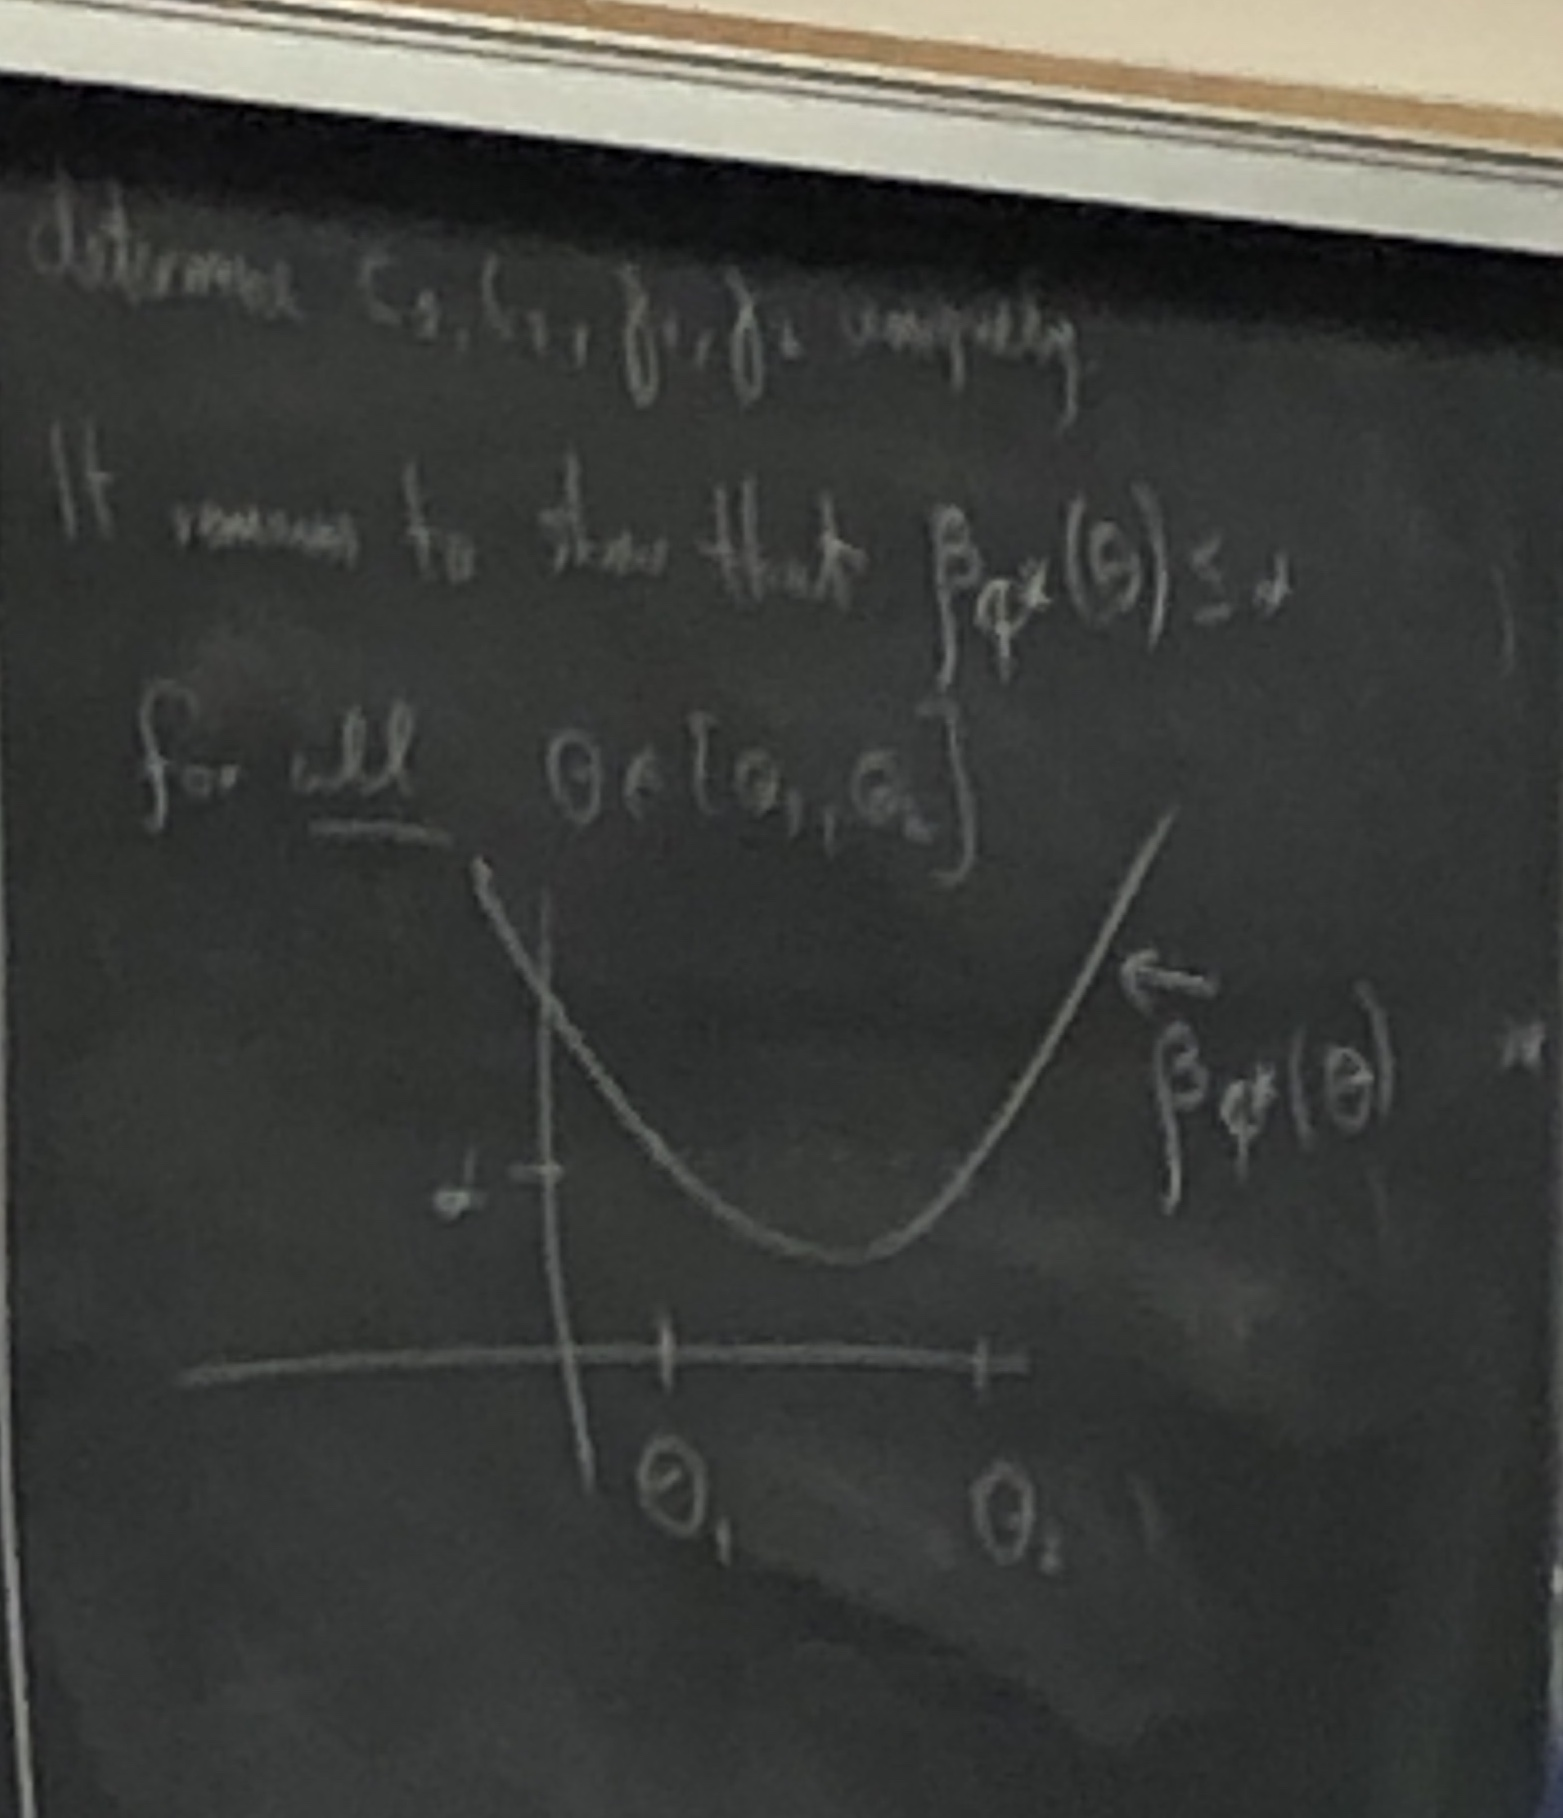
\includegraphics[scale=0.15]{mathstats_gnp_ex_3}
\caption{Third figure for Example \ref{mathstats.gnp.ex.prob}, the desired form of a power function for our selected test.}
\label{mathstats_gnp_ex_fig_3}
\end{center}
\end{figure}

\end{solution}

\begin{theorem}[\textbf{Theorem 3.7.1 in Lehmann and Romano}]

The most powerful unbiased test for a one-parameter exponential family is 

\[
\phi^*(x) = \begin{cases}
1, & T(x) < c_1 \text{ or } T(x) > c_2 \\
\gamma_1, & T(x) = c_1 \\
\gamma_2, & T(x) = c_2 \\
0, & T(x) \in (c_1, c_2)
\end{cases}
\]

such that 

\begin{enumerate}[(a)]

\item \(\E_{\theta_0}(\phi^*(X) = \alpha\).

\item \( \left. \deriv{}{\theta} \beta_{\phi^*}(\theta) \right|_{\theta = \theta_0} = 0\)  (\(\E_{\theta_0} T(X) \phi^*(X) = \alpha \E_{\theta_0} T(X)\)).

\end{enumerate}



\end{theorem}

\begin{proof}[Proof of constraint (b).]  For any unbiased test \(\phi\) of size \(\alpha\),



\[
p_\theta(x) = \frac{1}{c(\theta)} e^{\theta T(x)} = \tilde{c}(\theta)e^{\theta T(x)}
\]

(letting \( \tilde{c}(\theta) =  \frac{1}{c(\theta)}\)). Then 

\[
\beta_{\phi}(\theta) = \int \phi(x) p_\theta(x) d\mu = \int \phi(x) \tilde{c}(\theta) e^{\theta T(x)} \ d\mu
\]

so the derivative is

\begin{multline*}
\beta'_{\phi}(\theta) = \int \phi(x) [ \tilde{c}'(\theta) + T(x) \tilde{c}(\theta)] \tilde{c}(\theta) e^{\theta T(x)} \ d \mu
%\\ = \int \left[ \phi(x) p_\theta(x) d\mu 
%\\ = \int \phi(x) \tilde{c}'(\theta) e^{\theta T(x)}  + T(\alpha) \tilde{c}(\theta) e^{\theta T(x)} \right] \ d\mu = 0 
\\ = \frac{ \tilde{c}'(\theta)}{\tilde{c}(\theta)} \int \phi(x) \tilde{c}(\theta) e^{\theta T(x)} \ d\mu + \int \phi(x) T(x) \tilde{c}(\theta) e^{\theta T(x)} \ d \mu =  \frac{ \tilde{c}'(\theta)}{\tilde{c}(\theta)} \E_\theta \phi(X) + \E_\theta \phi(X) T(X)
\\ =  \frac{ \tilde{c}'(\theta)}{\tilde{c}(\theta)}  \alpha + \alpha \E_{\theta_0} T(x) = 0  \implies  \frac{ \tilde{c}'(\theta)}{\tilde{c}(\theta)}  = -E_{\theta_0} T(X)
\end{multline*}

Hence,

\[
 \frac{ \tilde{c}'(\theta)}{\tilde{c}(\theta)}  \underbrace{\E_{\theta_0}\phi(X)}_{\alpha} + \E_{\theta_0} \phi(X) T(X) = 0 
\]

implies that \(- \alpha \E_{\theta_0} T(X) + \E_{\theta_0} \phi(X) T(X) = 0 \) so it follows that \(\E_{\theta_0} T(X) \phi(X) = \alpha \E_{\theta_0} T(X)\). 

\[
\vdots
\]


For any unbiased test \(\phi\), \(\beta'_{\phi}(\theta) = 0\). (We know the test is unbiased: \(\phi_\alpha = \alpha\).) Plug \(\phi(x) = \alpha\) in to this equation to get 

\[
\frac{\tilde{c}'(\theta)}{\tilde{c}(\theta)} = -\E_{\theta_0} T(X).
\]

\end{proof}



\begin{example}

Let \(X_1, \ldots, X_n\) be i.i.d. \(\mathcal{N}(0, \sigma^2)\), \(\sigma^2 > 0\). Find the UMP unbiased test for \(H_0: \sigma^2 = \sigma_0^2\), \(H_a: \sigma^2 \neq \sigma_0^2\). Assuming that \(n\) is large, find the approximate values \(c_1 (\alpha)\), \(c_2 (\alpha)\).

\end{example}

Before solving this we will prove a lemma that we have been using implicitly.

\begin{lemma}

Suppose that \(T(X)\) is sufficient for \(\{p_\theta, \theta \in \Theta\}\), and let \(\phi\) be a test. Denote

\[
\psi(X) := \E_\theta [ \phi(X) \mid T(X)].
\]

Then 

\begin{enumerate}[(a)]

\item \(\psi(X)\) is a test.

\item \(\E_\theta \psi(X) = \E_\theta \phi(X)\). 

\end{enumerate}

\end{lemma}

\begin{proof}

\begin{enumerate}[(a)]

\item Since \(T(X)\) is sufficient, the expectation over \(\theta\) does not matter because we are conditioning on \(T(X)\) anyway. That is, the distribution of \(\phi(X)\) conditional on \(T(X)\) does not depend on \(\theta\). Therefore the expectation over \(\theta\) does not either. (A test takes values between 0 and 1 and doesn't depend on \(\theta\), only depends on the data.)

\item 

\[
\E_\theta \psi(X) = \E_\theta \left( \E_\theta [ \phi(X) \mid T(X)] \right) = \E_\theta \phi(X).
\]

\end{enumerate}

\end{proof}

\begin{definition}[\textbf{Boundably complete}]

\(T(X)\) is \textbf{boundably complete} if and only if for any function \(G\) such that \(|G| \leq 1\) (bounded), 

\[
 \left\{ \E_\theta G(T) = 0 \qquad \forall \theta \in \Theta \right\} \implies G(T) = 0 \text{ a.e.}
\] 

\end{definition}

So if a statistic is complete, it is boundably complete (if it is complete, the equation holds for all functions \(G\), not just bounded ones). Example: 

\[
X \in \{-1, 0, 1, 2, \ldots \}, \qquad
\mathbb{P}_\theta(X = k) = \begin{cases}
 \theta, & k = -1 \\
(1 - \theta)^2 \theta^k, & k \in \{0, 1, \ldots\}
\end{cases}
\]

Then \(T(X) = X\) is boundably complete but not complete.

We want to be able to work with distributions that are more than one dimensional. We can do this by reducing the family to a one-parameter family. We do this in the following way, with tests with Neyman structure. Assume we have \(X \sim P_\theta, \theta \in \Theta\). The problem is \(H_0: \theta \in \Theta_0, H_a: \theta \in \Theta_a\), where \(\Theta_B := \overline{\Theta}_0 \cap \overline{\Theta}_a\) (the intersection of the closures of these sets). 

\

Example: \(X_1, \ldots, X_n \sim \mathcal{N}(\mu, \sigma^2)\), \(H_0: \mu \leq 0, H_a: \mu > 0\). Then if we plot \(\mathbb{R}^2\) with \(\mu\) as the horizontal axis and \(\sigma^2\) as the vertical axis, the acceptance region is Quadrant II (including the top part of the vertical axis) and the rejection region is Quadrant I (not including the top part of the vertical axis). The boundary is the vertical axis (\(\Theta_B = \{\mathcal{N}(0, \sigma^2), \sigma^2 > 0\}\)).

\

Approach: take a complete sufficient statistic for the boundary family. We will condition on it and then find tests of size \(\alpha\). 


\begin{definition}
Let \(T(X)\) be sufficient for the boundary family \(\{p_{\theta}, \theta \in \Theta_B\}\). Test \(\phi\) has \textbf{Neyman structure with respect to \(T\)} if and only if for some \(\alpha \in [0,1]\)

\[
\E_\theta [\phi(X) \mid T(X)] = \alpha, \qquad \forall \theta \in \Theta_B.
\]


\end{definition}

Note that \(\phi\) has Neyman structure implies it is SOB of size \(\alpha\) (SOB means "similar on the boundary:" the power function is essentially constant on the boundary).

\begin{theorem}

All SOB tests of size \(\alpha\) have Neyman structure if and only if \(T\) is boundably complete (and sufficient).

\end{theorem}

\begin{proof}

First we will prove this direction: suppose that \(T\) is sufficient and boundably complete. Then

\[
\E_\theta \phi(X) = \alpha \qquad \forall \theta \in \Theta_B.
\]

But then 

\begin{multline*}
\alpha = \E_\theta \phi(X) = \E_\theta \E[\phi(X) \mid T(X)] = \E_\theta G(T)  \implies \E_\theta(G(T) - \alpha) = 0 , \qquad \theta \in \Theta_0
\\ \implies G(T) - \alpha = 0 \text{ a.s.}  \qquad \implies G(T) = \alpha \text { a.s.}
\end{multline*}

so the result follows. (Note that we only need boundable completeness since we must have \(0 \leq |G| \leq 1 \forall T\).) Next, assume that all SOB tests of size \(\alpha\) have Neyman structure. We will prove by contradiction that then \(T\) must be boundably complete. Suppose \(T\) is not boundably complete. Then there must exist some function \(\psi\) such that \(|\psi| \leq 1\) and \(\E_\theta \psi(T) = 0 \ \forall \theta \in \Theta_B\) but \(\psi(T)\) is not identically 0. Define \(\phi := \alpha + c \psi(T)\), where we choose \(c \neq 0 \) such that \( 0 \leq |\phi | \leq 1\) so that \(\phi\) is a test. Note that \(\E_\theta \phi = \alpha\) for all \(\theta \in \Theta_B\), so \(\phi\) is SOB of size \(\alpha\) (it is SOB because this result holds for all \(\theta \in \Theta_B\), where \(\Theta_B\) is the boundary family). But

\[
\E( \phi(x) \mid T(x) ) = \alpha + c \psi(T(x)) \neq \alpha
\]

since \(\psi\) is not identically 0 by assumption.

\end{proof}

\begin{theorem}\label{mathstats.541a.ex.5.10.thm}

Assume that \(X \sim P_\theta\) where 

\[
p_\theta(x) = \frac{1}{c(\theta)} h(x) \cdot \exp \left\{  \sum_{j=1}^k \theta_j T_j(x) \right\} 
\]

(canonical exponential family). Then \(T(X) = (T_1(X), \ldots, T_k(X))\) is a sufficient statistic for the family \(\{p_\theta, \theta \in \Theta\}\) provided that \(\Theta\) has non-empty interior. (See also Proposition \ref{mathstats.541a.ex.5.10}.)

\end{theorem}

Conditioning method: assume that \(\beta_\phi(\theta)\) is continuous for any test \(\phi\). 

\begin{enumerate}[(1)]

\item \(\phi\) is unbiased, so \(\phi\) is SOB.

\item UMP SOB test of size \(\alpha\) is UMP unbiased test of size \(\alpha\). 

\item Neyman structure implies that it suffices to find the test that maximizes the conditional power \(\E_\theta(\phi \mid T) \) for all \(\theta \in \Theta_a\). 

\end{enumerate}

\begin{example}

\(X \sim \operatorname{Poisson}(\mu)\), \(Y \sim \operatorname{Poisson}(\nu)\). \(H_0: \mu \leq \nu\), \(H_a: \nu > \nu\). Find the UMP unbiased test.

\end{example}

\begin{solution}

\[
p_{\mu, \nu}(x,y) = \frac{e^{-(\mu + \nu)} \mu^x \nu^y}{x!y!} = e^{-(\mu + \nu)} e^{x \log \mu + y \log \nu} \cdot \frac{1}{x!y!} 
=  \frac{1}{x!y!}  e^{-(\mu + \nu)} e^{x \log (\mu/\nu) + (x+ y) \log \nu} 
\]

Let \(\xi := \log(\mu/\nu), \eta = \log \nu\). Then \(H_0: \xi \leq 0\), \(H_a: \xi > 0\). We can use an SOB thing where \(\Theta_B = \{ (\xi, \eta) : \eta = 0\}\) is the boundary family. Then \(T(X,Y) = X + Y \) is complete sufficient for the boundary family \(\{p_{\xi, \eta} : \xi = 0\}\) by Theorem \ref{mathstats.541a.ex.5.10.thm} (Proposition \ref{mathstats.541a.ex.5.10}). Let's condition everything on \(T = X + Y\). We need to find \(\mathbb{P}(X =x \mid T = t)\). Note that

\[
\mathbb{P}_{\mu, \nu} (X = x \mid T = t) = \frac{\mathbb{P}_{\mu, \nu} (X = x , Y = t - x) }{\mathbb{P}_{\mu, \nu} (T = t) } = \frac{\mu^x}{x!} e^{-\mu} \cdot \frac{ \nu^{t-x}}{(t-x)!} e^{-\nu} \cdot \frac{t! e^{\mu + \nu} }{(\mu + \nu)^t}
\]

where we used \(T \sim \operatorname{Poisson}(\mu + \nu)\) (exercise; use characteristic functions)

\[
= \binom{t}{x} \left( \frac{\mu}{\mu + \nu} \right)^x \left( \frac{\nu}{\mu + \nu} \right)^{t-x}
\]

so \(\{X \mid T = t\} \sim \operatorname{Bin}(t, \mu/(\mu + \nu))\). 

Note that \(\mu \leq \nu \iff p \leq 1/2\), so for our new problem, we have \(X \sim \operatorname{Binom}(t, p)\), and we will test \(H_0': p \leq 1/2, H_a': p > 1/2\). For this problem we can find the UMP test (not just the UMP unbiased test) because the binomial family has a monotone likelihood ratio with respect to \(T(X) = X\) when \(p \in (0,1)\) and \(t\) fixed (very straightforward to check). 

Then

\[
\phi(x) = \begin{cases}
1, & x > c(t) \\
\gamma, & x = c(t) \\
0, & x < c(t)
\end{cases}
\]

is UMP. To find \(c(t, \alpha)\), use

\begin{equation}\label{mathstats.poiss.ex.ump.test}
\E_{p = 1/2} \phi(X) = \alpha \iff \sum_{x > c(t)} \binom{t}{x} (1/2)^t + \gamma \binom{t}{c(t)} (1/2)^{c(t)} = \alpha.
\end{equation}

(hard to compute in practice; need a computer). So the test for the original problem is 

\[
\phi(X, Y) = \begin{cases}
1, & X > c(t) \\
\gamma, & x =c(t) \\
0, x < c(t)
\end{cases}
\]

where \(t = X + Y\) and \(c(t)\) solves (\ref{mathstats.poiss.ex.ump.test}).

\end{solution}



%
%
%
%
%
%
%



\begin{proposition}[\textbf{Stats 100B Homework problem}] Let \(Y_1, Y_2, \ldots, Y_n\) be the outcomes of \(n\) independent Bernoulli trials. Then by the Neyman-Pearson lemma, the best critical region for testing

\[
H_0: p = p_0 \ \ \ \ \ \ \ H_a: p > p_0
\]

is

\[
\frac{y}{n} = \frac{1}{n}\sum Y_i  > \frac{\log(K) + n \log \bigg( \frac{1 - p_a}{1 - p_0} \bigg)}{n\log \bigg( \frac{p_0(1 - p_a)}{p_a(1 - p_0)} \bigg)}.
\]

\end{proposition}

\begin{proof}

\[
\Pr(\sum Y_i = y) = {n \choose y}p^y(1-p)^{n-y}
\]

Using the Neyman-Pearson lemma (let \(p_a\) be some particular value of \(p > p_0\)):

\[
\frac{L(p_0)}{L(p_a)} = \frac{{n \choose y}p_0^y(1-p_0)^{n-y}}{{n \choose y}p_a^y(1-p_a)^{n-y}} < K
\]

\[
\bigg( \frac{p_0}{p_a} \bigg) ^y   \bigg( \frac{1 - p_0}{1 - p_a} \bigg)^{n} \bigg( \frac{1 - p_0}{1 - p_a} \bigg)^{-y}  < K
\]

\[
\bigg( \frac{p_0(1 - p_a)}{p_a(1 - p_0)} \bigg) ^y  < K  \bigg( \frac{1 - p_a}{1 - p_0} \bigg)^{n} 
\]

\[
y \log \bigg( \frac{p_0(1 - p_a)}{p_a(1 - p_0)} \bigg) < \log(K) + n \log \bigg( \frac{1 - p_a}{1 - p_0} \bigg)
\]

Aside:

\[
\frac{p_0(1 - p_a)}{p_a(1 - p_0)} = \frac{p_0 - p_0 p_a}{p_a - p_0 p_a} < 1
\]

since by assumption \(p_a > p_0\). Therefore \( \log \bigg( \frac{p_0(1 - p_a)}{p_a(1 - p_0)} \bigg) < 0 \). So we have

\[
\frac{y}{n} = \frac{1}{n}\sum Y_i  > \frac{\log(K) + n \log \bigg( \frac{1 - p_a}{1 - p_0} \bigg)}{n\log \bigg( \frac{p_0(1 - p_a)}{p_a(1 - p_0)} \bigg)}
\]

as the form for our critical region.

\end{proof}




%\bibliographystyle{abbrvnat}
%\bibliography{mybib2fin}
%\end{document}







